%%%%%%%%%%%%%%%%%%%% book.tex %%%%%%%%%%%%%%%%%%%%%%%%%%%%%
%
% sample root file for the chapters of your "monograph"
%
% Use this file as a template for your own input.
%
%%%%%%%%%%%%%%%% Springer-Verlag %%%%%%%%%%%%%%%%%%%%%%%%%%


% RECOMMENDED %%%%%%%%%%%%%%%%%%%%%%%%%%%%%%%%%%%%%%%%%%%%%%%%%%%
\documentclass[envcountsame,envcountchap,openany]{svmono}
%\documentclass[11pt]{book} 
% teste
%\usepackage[dvinames]{xcolor}
% Measurements are taken directly from the guide
\usepackage[top=1in,left=1.5in,bottom=1in,right=2.5cm]{geometry}
%\usepackage{graphicx}
%\usepackage[colorlinks=false,
%            pdfborder={0 0 0},
%            ]{hyperref}
%\usepackage{lipsum}
\usepackage[absolute]{textpos}
\usepackage[table]{xcolor}
\usepackage{tikz}
\usetikzlibrary{calc}
\usepackage{scrextend}
\usepackage{tabularx}
\usepackage{spreadtab}

% A nice serif font, but no the prescribed nonfree ITC stone
%\usepackage[oldstylenums]{kpfonts}
\usepackage[T1]{fontenc}
\usepackage[utf8]{inputenc}
\usepackage[portuguese]{babel}
\usepackage{enumerate}
\usepackage{multirow}
\usepackage[titletoc,toc,page]{appendix}
\usepackage{pdfpages}
%\usepackage[titletoc]{appendix}
%\renewcommand{\appendixtocname}{Anexos}
\renewcommand{\appendixtocname}{Anexos}
\renewcommand{\appendixpagename}{Anexos}

\newcounter{artigo}
\newcommand{\artigo}{\refstepcounter{artigo} % 
	\ifnum\theartigo<10 %
	{\bfseries Art.~\arabic{artigo}º~--~}%
	\else
	{\bfseries Art. \arabic{artigo}~--~}%
	\fi
	%Art. \arabic{artigo}.~
	}
\newcounter{paragrafo}
\newcommand{\paragrafo}{\refstepcounter{paragrafo} % 
	\S~\arabic{paragrafo}º~%
}

\newenvironment{paragrafos}{\setcounter{paragrafo}{0}
	\setlength{\parindent}{0pt}
	\begin{addmargin}[4em]{0pt} 
	}
	{\end{addmargin}
		}

\newenvironment{itquotation}
{\begin{quotation}\itshape}
{\end{quotation}}	
% No paragraph indentation
\parindent0pt
\setlength{\parskip}{0.8\baselineskip}
%\raggedright
%\pagestyle{empty}

%fim teste
% choose options for [] as required from the list
% in the Reference Guide, Sect. 2.2

\usepackage{makeidx}         % allows index generation
\usepackage{graphicx}        % standard LaTeX graphics tool
                             % when including figure files
\usepackage{multicol}        % used for the two-column index
\usepackage[bottom]{footmisc}% places footnotes at page bottom

% etc.
% see the list of further useful packages
% in the Reference Guide, Sects. 2.3, 3.1-3.3

\makeindex             % used for the subject index
                       % please use the style svind.ist with
                       % your makeindex program

% Nomes das Disciplinas

% Nomes das Disciplinas %%%%%%%%%%%%%%%%%%%%%%%%%%%%%%%%%%%%%%%%%%%%%%%%%%%%%%%%%%%%%%%%%%%%
\newcommand{\AlgLin}{Álgebra Linear III}
\newcommand{\AlgLinSName}{Álgebra Linear III}
\newcommand{\AlgLinCod}{IME 02-01388}
\newcommand{\AlgLinCH}{75}
\newcommand{\AlgLinCred}{5}

\newcommand{\AnaVet}{Análise Vetorial}
\newcommand{\AnaVetSName}{Análise Vetorial}
\newcommand{\AnaVetCod}{IME 02-04629}
\newcommand{\AnaVetCH}{60}
\newcommand{\AnaVetCred}{4}

\newcommand{\CalcI}{Cálculo Diferencial e Integral I}
\newcommand{\CalcISName}{Cálculo Dif. e Integral I}
\newcommand{\CalcICod}{IME 01-00508}
\newcommand{\CalcICH}{75}
\newcommand{\CalcICred}{5}

\newcommand{\CalcII}{Cálculo Diferencial e Integral II}
\newcommand{\CalcIISName}{Cálculo Dif. e Integral II}
\newcommand{\CalcIICod}{IME 01-00854}
\newcommand{\CalcIICH}{75}
\newcommand{\CalcIICred}{5}

\newcommand{\CalcIII}{Cálculo Diferencial e Integral III}
\newcommand{\CalcIIISName}{Cálculo Dif. e Integral III}
\newcommand{\CalcIIICod}{IME 01-03646}
\newcommand{\CalcIIICH}{75}
\newcommand{\CalcIIICred}{5}

\newcommand{\DesBas}{Desenho Básico}
\newcommand{\DesBasSName}{Desenho Básico}
\newcommand{\DesBasCod}{IME 03-00587}
\newcommand{\DesBasCH}{60}
\newcommand{\DesBasCred}{3}

\newcommand{\FisI}{Física Teórica e Experimental I}
\newcommand{\FisISName}{Física Teórica e Experim. I}
\newcommand{\FisICod}{FIS 01-05095}
\newcommand{\FisICH}{105}
\newcommand{\FisICred}{5}

\newcommand{\FisII}{Física Teórica e Experimental II}
\newcommand{\FisIISName}{Física Teórica e Experim. II}
\newcommand{\FisIICod}{FIS 02-05143}
\newcommand{\FisIICH}{105}
\newcommand{\FisIICred}{5}

\newcommand{\FisIII}{Física Teórica e Experimental III}
\newcommand{\FisIIISName}{Física Teórica e Experim. III}
\newcommand{\FisIIICod}{FIS 03-05185}
\newcommand{\FisIIICH}{120}
\newcommand{\FisIIICred}{6}

\newcommand{\FisIV}{Física Teórica e Experimental IV}
\newcommand{\FisIVSName}{Física Teórica e Experim. IV}
\newcommand{\FisIVCod}{FIS 04-05212}
\newcommand{\FisIVCH}{120}
\newcommand{\FisIVCred}{6}

\newcommand{\GD}{Geometria Descritiva I}
\newcommand{\GDSName}{Geometria Descritiva I}
\newcommand{\GDCod}{IME 03-02046}
\newcommand{\GDCH}{60}
\newcommand{\GDCred}{3}

\newcommand{\GeoAna}{Geometria Analítica e Cálculo Vetorial I}
\newcommand{\GeoAnaSName}{Geom. Analít. e Cálc. Vet. I}
\newcommand{\GeoAnaCod}{IME 03-01913}
\newcommand{\GeoAnaCH}{75}
\newcommand{\GeoAnaCred}{5}

\newcommand{\MecTec}{Mecânica Técnica}
\newcommand{\MecTecSName}{Mecânica Técnica}
\newcommand{\MecTecCod}{FEN 03-05787}
\newcommand{\MecTecCH}{60}
\newcommand{\MecTecCred}{4}

\newcommand{\ProbEst}{Probabilidade e Estatística III}
\newcommand{\ProbEstSName}{Probabilidade e Estatística III}
\newcommand{\ProbEstCod}{IME 05-05316}
\newcommand{\ProbEstCH}{75}
\newcommand{\ProbEstCred}{5}

\newcommand{\QuiX}{Química X}
\newcommand{\QuiXSName}{Química X}
\newcommand{\QuiXCod}{QUI 07-03793}
\newcommand{\QuiXCH}{60}
\newcommand{\QuiXCred}{3}

\newcommand{\Adm}{Administração Aplicada à Engenharia III}
\newcommand{\AdmSName}{Adm. Aplic. À Engenharia III}
\newcommand{\AdmCod}{FAF 03-04439}
\newcommand{\AdmCH}{60}
\newcommand{\AdmCred}{3}

\newcommand{\AnaFis}{Análise de Sistemas Físicos I}
\newcommand{\AnaFisSName}{Análise de Sistemas Físicos I}
\newcommand{\AnaFisCod}{FEN 04-05253}
\newcommand{\AnaFisCH}{75}
\newcommand{\AnaFisCred}{4}

\newcommand{\CEV}{Circuitos Elétricos V}
\newcommand{\CEVSName}{Circuitos Elétricos V}
\newcommand{\CEVCod}{FEN 04-xxxxx}
\newcommand{\CEVCH}{90}
\newcommand{\CEVCred}{4}

\newcommand{\CEVI}{Circuitos Elétricos VI}
\newcommand{\CEVISName}{Circuitos Elétricos VI}
\newcommand{\CEVICod}{FEN 04-xxxxx}
\newcommand{\CEVICH}{90}
\newcommand{\CEVICred}{4}

\newcommand{\CServMec}{Controle e Servomecanismos III}
\newcommand{\CServMecSName}{Controle e Servomecanismos III}
\newcommand{\CServMecCod}{FEN 05-05025}
\newcommand{\CServMecCH}{75}
\newcommand{\CServMecCred}{4}

\newcommand{\EletI}{Eletrônica I}
\newcommand{\EletISName}{Eletrônica I}
\newcommand{\EletICod}{FEN 05-01620}
\newcommand{\EletICH}{90}
\newcommand{\EletICred}{4}

\newcommand{\EletII}{Eletrônica II}
\newcommand{\EletIISName}{Eletrônica II}
\newcommand{\EletIICod}{FEN 05-01840}
\newcommand{\EletIICH}{90}
\newcommand{\EletIICred}{4}

\newcommand{\EletIIA}{Eletrônica II-A}
\newcommand{\EletIIASName}{Eletrônica II-A}
\newcommand{\EletIIACod}{FEN 05-xxxx}
\newcommand{\EletIIACH}{90}
\newcommand{\EletIIACred}{4}

\newcommand{\FenTran}{Fenômenos de Transporte}
\newcommand{\FenTranSName}{Fenômenos de Transporte}
\newcommand{\FenTranCod}{FEN 03-02040}
\newcommand{\FenTranCH}{60}
\newcommand{\FenTranCred}{3}

\newcommand{\IntEco}{Introdução à Economia III}
\newcommand{\IntEcoSName}{Introdução à Economia III}
\newcommand{\IntEcoCod}{FCE 02-04657}
\newcommand{\IntEcoCH}{60}
\newcommand{\IntEcoCred}{4}

\newcommand{\IntAmb}{Introdução à Engenharia Ambiental}
\newcommand{\IntAmbSName}{Introd. à Eng. Ambiental}
\newcommand{\IntAmbCod}{FEN 07-02162}
\newcommand{\IntAmbCH}{60}
\newcommand{\IntAmbCred}{3}

\newcommand{\MatEle}{Materiais Elétricos e Magnéticos I}
\newcommand{\MatEleSName}{Mat. Elét. e Magnéticos I}
\newcommand{\MatEleCod}{FEN 04-05197}
\newcommand{\MatEleCH}{60}
\newcommand{\MatEleCred}{3}

\newcommand{\ModMat}{Modelos Matemáticos III}
\newcommand{\ModMatSName}{Modelos Matemáticos III}
\newcommand{\ModMatCod}{FEN 05-04923}
\newcommand{\ModMatCH}{75}
\newcommand{\ModMatCred}{4}

\newcommand{\MetQuant}{Métodos Quantitativos Aplicados em Produção I}
\newcommand{\MetQuantSName}{Métodos Quant. Aplic. em Produção I}
\newcommand{\MetQuantCod}{FEN 09-7345}
\newcommand{\MetQuantCH}{45}
\newcommand{\MetQuantCred}{3}

\newcommand{\PrincTelec}{Princípios de Telecomunicações III}
\newcommand{\PrincTelecSName}{Princípios de Telec. III}
\newcommand{\PrincTelecCod}{FEN 05-04975}
\newcommand{\PrincTelecCH}{75}
\newcommand{\PrincTelecCred}{4}

\newcommand{\ResMat}{Resistência dos Materiais Básica}
\newcommand{\ResMatSName}{Resistência dos Mat. Básica}
\newcommand{\ResMatCod}{FEN 01-04833}
\newcommand{\ResMatCH}{60}
\newcommand{\ResMatCred}{3}

\newcommand{\SegHig}{Engenharia do Trabalho I}
\newcommand{\SegHigSName}{Engenharia do Trabalho I}
\newcommand{\SegHigCod}{FEN 09-5255}
\newcommand{\SegHigCH}{60}
\newcommand{\SegHigCred}{3}

\newcommand{\AlgComp}{Algoritmos Computacionais I}
\newcommand{\AlgCompSName}{Algoritmos Computac. I}
\newcommand{\AlgCompCod}{FEN 06-xxxx}
\newcommand{\AlgCompCH}{75}
\newcommand{\AlgCompCred}{4}

\newcommand{\AnAlg}{Análise de Algoritmos I}
\newcommand{\AnAlgSName}{Análise de Algoritmos I}
\newcommand{\AnAlgCod}{FEN 06-xxxx}
\newcommand{\AnAlgCH}{60}
\newcommand{\AnAlgCred}{4}

\newcommand{\ArqComp}{Arquitetura de Computadores A}
\newcommand{\ArqCompSName}{Arquitetura de Computadores A}
\newcommand{\ArqCompCod}{FEN 06-xxxx}
\newcommand{\ArqCompCH}{75}
\newcommand{\ArqCompCred}{4}

\newcommand{\Control}{Controle de Processos por Computador I}
\newcommand{\ControlSName}{Controle de Processos por Computador I}
\newcommand{\ControlCod}{FEN 06-xxxx}
\newcommand{\ControlCH}{75}
\newcommand{\ControlCred}{4}

\newcommand{\EngComput}{Engenharia Computacional}
\newcommand{\EngComputSName}{Engenharia Computacional}
\newcommand{\EngComputCod}{FEN 06-xxxx}
\newcommand{\EngComputCH}{75}
\newcommand{\EngComputCred}{4}

\newcommand{\EngCompSoc}{Engenharia de Computação e Sociedade}
\newcommand{\EngCompSocSName}{Engenharia de Computação e Sociedade}
\newcommand{\EngCompSocCod}{FEN 06-xxxx}
\newcommand{\EngCompSocCH}{60}
\newcommand{\EngCompSocCred}{4}

\newcommand{\EngSistA}{Engenharia de Sistemas}
\newcommand{\EngSistASName}{Engenharia de Sistemas}
\newcommand{\EngSistACod}{FEN 06-xxxx}
\newcommand{\EngSistACH}{60}
\newcommand{\EngSistACred}{4}

\newcommand{\ProjBD}{Projeto e Administração de Banco de Dados}
\newcommand{\ProjBDSName}{Projeto e Adm. de Banco de Dados}
\newcommand{\ProjBDCod}{FEN 06-xxxx}
\newcommand{\ProjBDCH}{60}
\newcommand{\ProjBDCred}{4}

\newcommand{\EstSup}{Estágio Supervisionado XI-A}
\newcommand{\EstSupSName}{Estágio Supervisionado XI-A}
\newcommand{\EstSupCod}{FEN 06-xxxx}
\newcommand{\EstSupCH}{300}
\newcommand{\EstSupCred}{10}

\newcommand{\EstrInf}{Estruturas de Informação A}
\newcommand{\EstrInfSName}{Estruturas de Informação A}
\newcommand{\EstrInfCod}{FEN 06-xxxx}
\newcommand{\EstrInfCH}{75}
\newcommand{\EstrInfCred}{4}

\newcommand{\FundComp}{Fundamentos de Computadores}
\newcommand{\FundCompSName}{Fundamentos de Computadores}
\newcommand{\FundCompCod}{FEN 06-xxxx}
\newcommand{\FundCompCH}{90}
\newcommand{\FundCompCred}{5}

\newcommand{\IC}{Inteligência Computacional}
\newcommand{\ICSName}{Inteligência Computacional}
\newcommand{\ICCod}{FEN 06-xxxx}
\newcommand{\ICCH}{60}
\newcommand{\ICCred}{4}

\newcommand{\LabProgA}{Laboratório de Programação A}
\newcommand{\LabProgASName}{Laboratório de Programação A}
\newcommand{\LabProgACod}{FEN 06-xxxx}
\newcommand{\LabProgACH}{75}
\newcommand{\LabProgACred}{4}

\newcommand{\LabProgB}{Laboratório de Programação B}
\newcommand{\LabProgBSName}{Laboratório de Programação B}
\newcommand{\LabProgBCod}{FEN 06-xxxx}
\newcommand{\LabProgBCH}{75}
\newcommand{\LabProgBCred}{4}

\newcommand{\LogProg}{Lógica em Programação}
\newcommand{\LogProgSName}{Lógica em Programação}
\newcommand{\LogProgCod}{FEN 06-xxxx}
\newcommand{\LogProgCH}{60}
\newcommand{\LogProgCred}{4}

\newcommand{\MineraDados}{Mineração de Dados}
\newcommand{\MineraDadosSName}{Mineração de Dados}
\newcommand{\MineraDadosCod}{FEN 06-xxxx}
\newcommand{\MineraDadosCH}{60}
\newcommand{\MineraDadosCred}{3}

\newcommand{\ProcImag}{Processamento de Imagens}
\newcommand{\ProcImagSName}{Processamento de Imagens}
\newcommand{\ProcImagCod}{FEN 06-xxxx}
\newcommand{\ProcImagCH}{60}
\newcommand{\ProcImagCred}{3}

\newcommand{\CompParal}{Computação Paralela e Distribuída}
\newcommand{\CompParalSName}{Computação Paralela e Distribuída}
\newcommand{\CompParalCod}{FEN 06-xxxx}
\newcommand{\CompParalCH}{75}
\newcommand{\CompParalCred}{4}

\newcommand{\ProjA}{Projeto de Graduação XI-A}
\newcommand{\ProjASName}{Projeto de Graduação XI-A}
\newcommand{\ProjACod}{FEN 06-04578}
\newcommand{\ProjACH}{45}
\newcommand{\ProjACred}{2}

\newcommand{\ProjB}{Projeto de Graduação XI-B}
\newcommand{\ProjBSName}{Projeto de Graduação XI-B}
\newcommand{\ProjBCod}{FEN 06-04635}
\newcommand{\ProjBCH}{45}
\newcommand{\ProjBCred}{2}

\newcommand{\ProjSO}{Projeto de Sistemas Operacionais}
\newcommand{\ProjSOSName}{Projeto de Sistemas Operacionais}
\newcommand{\ProjSOCod}{FEN 06-xxxx}
\newcommand{\ProjSOCH}{75}
\newcommand{\ProjSOCred}{5}

\newcommand{\SistEmb}{Sistemas Embutidos}
\newcommand{\SistEmbSName}{Sistemas Embutidos}
\newcommand{\SistEmbCod}{FEN 06-xxxx}
\newcommand{\SistEmbCH}{60}
\newcommand{\SistEmbCred}{3}

\newcommand{\Telep}{Teleprocessamento e Redes de Computadores I}
\newcommand{\TelepSName}{Teleproc. e Redes de Computadores I}
\newcommand{\TelepCod}{FEN 06-xxxx}
\newcommand{\TelepCH}{60}
\newcommand{\TelepCred}{4}

\newcommand{\TeoComp}{Teoria de Compiladores I}
\newcommand{\TeoCompSName}{Teoria de Compiladores I}
\newcommand{\TeoCompCod}{FEN 06-xxxx}
\newcommand{\TeoCompCH}{75}
\newcommand{\TeoCompCred}{5}

\newcommand{\EletA}{Eletiva A}
\newcommand{\EletASName}{Eletiva A}
\newcommand{\EletACod}{FEN 06-xxxx}
\newcommand{\EletACH}{60}
\newcommand{\EletACred}{3}

\newcommand{\EletB}{Eletiva B}
\newcommand{\EletBSName}{Eletiva B}
\newcommand{\EletBCod}{FEN 06-xxxx}
\newcommand{\EletBCH}{60}
\newcommand{\EletBCred}{3}

\newcommand{\EletC}{Eletiva C}
\newcommand{\EletCSName}{Eletiva C}
\newcommand{\EletCCod}{FEN 06-xxxx}
\newcommand{\EletCCH}{60}
\newcommand{\EletCCred}{3}


 %%%%%%%%%%%%%%%%%%%%%%%%%%%%%%%%%%%%%%%%%%%%%%%%%%%%%%%%%%%%%%%%%%%%
%Básico
\normalsize 

\begin{document}

\begin{textblock*}{3cm}[0.5,0.5](4cm,4cm)
    
\includegraphics[width=3cm]{imagens/logo_uerj_cor.jpg}
\end{textblock*}
\begin{textblock*}{12cm}(6cm,3cm)   % 6.375=8.5 - 1.5 - 0.625
    Universidade do Estado do Rio de Janeiro\\
    Sub-Reitoria de Graduação \\
    Faculdade de Engenharia\\
    Departamento de Engenharia de Sistemas e Computação
\end{textblock*}



\title{Projeto Pedagógico do Curso de Engenharia de Computação}
\subtitle{2016}
\date{}
\maketitle


\begin{minipage}{\textwidth}
\vfill
\tableofcontents
\end{minipage}
\frontmatter%%%%%%%%%%%%%%%%%%%%%%%%%%%%%%%%%%%%%%%%%%%%%%%%%%%%%%
%\include{dedic}
%\include{pref} 

%\tableofcontents


\mainmatter%%%%%%%%%%%%%%%%%%%%%%%%%%%%%%%%%%%%%%%%%%%%%%%%%%%%%%%
%\include{part}
%%%%%%%%%%%%%%%%%%%%% chapter.tex %%%%%%%%%%%%%%%%%%%%%%%%%%%%%%%%%
%
% sample chapter
%
% Use this file as a template for your own input.
%
%%%%%%%%%%%%%%%%%%%%%%%% Springer-Verlag %%%%%%%%%%%%%%%%%%%%%%%%%%


\chapter{Introdução}
\label{intro} % Always give a unique label
% use \chaptermark{}
% to alter or adjust the chapter heading in the running head

Este documento apresenta o projeto da estrutura curricular de um novo curso de \textbf{Engenharia de Computação} da Universidade do Estado do Rio de Janeiro. Tal curso será oferecido pelo \textbf{Departamento de Engenharia de Sistemas e Computação} (DESC) da \textbf{Faculdade de Engenharia} (FEN). O DESC oferece o curso de Engenharia Elétrica com Ênfase em Sistemas e Computação desde 1977, sendo, portanto, o primeiro no Brasil a oferecer graduação na área de Engenharia de Computação. Este curso sofreu uma reformulação significativa no início da década de 1990 e desde então permanece com o mesmo currículo, sem modificações. O objetivo agora é promover uma reforma desse curso e ofertá-lo como uma nova habilitação da engenharia.

A Engenharia, e principalmente a Engenharia de Computação, evolui rapidamente no mundo contemporâneo. Passados mais de 20 anos desde sua última reforma, urge adequar o curso aos novos tempos.

A motivação para oferecer o curso de \textbf{Engenharia de Computação} como uma nova habilitação da engenharia é torná-lo mais atual, em face às demandas da sociedade, para o desenvolvimento científico e tecnológico nos setores industrial e de serviços. Atualmente (2015), por ocasião do vestibular, os candidatos aos cursos da FEN têm a opção, entre outras habilitações, da Engenharia Elétrica. Assim, ao escolherem o curso de Engenharia Elétrica e em seguida optarem pela Ênfase em Sistemas e Computação terão, quando formados, diplomas de Engenheiros Eletricistas. Todavia a formação nos dias de hoje necessita de um maior conhecimento de certos conteúdos no desenvolvimento de sistemas e dispositivos computacionais, conforme as diretrizes do ENADE de 2014.

Outra motivação para oferecer o curso de \textbf{Engenharia de Computação} como uma nova habilitação da engenharia é tornar mais coerente a formação dos alunos da computação, pois o atual curso de Engenharia Elétrica com Ênfase em Sistemas e Computação prepara os seus alunos para atuarem como desenvolvedores  de sistemas de computação, criando software ou projetando hardware. Os egressos desse curso não teriam competência para, por exemplo, projetar sistemas de potência, que a habilitação Engenharia Elétrica poderia sugerir. Tal situação já acarretou diversos problemas aos alunos ao realizarem o ENADE, pois eles ficam mal posicionados, já que não cursaram disciplinas mais específicas da área elétrica.

Além das motivações para se criar um curso de Engenharia de Computação como uma habilitação única, tal projeto pedagógico visa apresentar uma atualização do currículo dentro da área da computação em face das mudanças tecnológicas ocorridas ao longo do tempo desde a última reforma do curso de Engenharia Elétrica com Ênfase em Sistemas e Computação, por volta dos anos 1990.


\chapter{Dados da UERJ}

\begin{description}
\item[Mantenedor:] Governo do Estado do Rio de Janeiro.
\item [Mantida:] Faculdade de Engenharia – Universidade do Estado do Rio de Janeiro.
\item [Local de Funcionamento:] Rua São Francisco Xavier 524, quinto andar, Maracanã, Rio de Janeiro – RJ.
\item [Reitor:] Ruy Garcia Marques.
\item [Vice-Reitora:] Maria Georgina Muniz Washington.
\item [Sub-Reitora de Graduação (SR1):] Tania Maria de Castro Carvalho Netto.
\item [Sub-Reitor de Pós-graduação e Pesquisa (SR2):] Egberto Gaspar de Moura.
\item [Sub-Reitora de Extensão e Cultura (SR3):] Elaine Ferreira Torres.
\item [Diretor do Centro de Tecnologia e Ciências:] Luis Antonio Campinho Pereira da Mota .
\item [Diretor da Faculdade de Engenharia:] Jorge Duarte Pires Valerio.
\end{description}

% Always give a unique label
% and use \ref{<label>} for cross-references
% and \cite{<label>} for bibliographic references
% use \sectionmark{}
% to alter or adjust the section heading in the running head
%Your text goes here. Use the \LaTeX\ automatism for your citations
%\cite{monograph}.

\section{Cursos Oferecidos pela FEN}
A tabela  ~\ref{tabvagas} apresenta as vagas oferecidas para o vestibular pela Faculdade de Engenharia da Universidade do Estado do Rio de Janeiro, campus Maracanã, para o primeiro e para o segundo semestre.
\label{sec:cursosoferecidos}

\setlength{\tabcolsep}{5pt}
\begin{table}
\centering
\caption{Vagas Oferecidas no 1º e no 2º semestre}
\label{tabvagas}
\renewcommand{\arraystretch}{1.5}
\begin{tabularx}{\textwidth}{|X|c|c|c|c|}
\hline
\multirow{2}{*}{\textbf{Habilitação}} & \multirow{2}{*}{\textbf{Turno}} & \multicolumn{2}{|c|}{\textbf{Vagas}} & \multirow{2}{*}{\textbf{Total}} \\\cline{3-4}
 & & \textbf{1º Sem.} & \textbf{2º Sem.} & \\
 \hline
 Engenharia Ambiental 
 e Sanitária  & Manhã/Tarde & 40  & -- &   \\
  & Tarde/Noite & -- & 40 & 80 \\
\hline
Engenharia Cartográfica & Manhã/Tarde & 20  & -- &   \\
& Tarde/Noite & -- & 20 & 40 \\
 \hline
Engenharia Civil & Manhã/Tarde & 60  & -- &   \\
(Construção Civil/Transportes/Estruturas)  & Tarde/Noite & -- & 60 & 120 \\
 \hline
Engenharia de Produção & Manhã/Tarde & 40  & -- &   \\
& Tarde/Noite & -- & 40 & 80 \\
\hline
Engenharia Elétrica (Sistemas e Computação/
& Manhã/Tarde & 100  & -- &   \\
 Sist. de Potência/Sist. Eletrônicos/Telecomunicações)& Tarde/Noite & -- & 100 & 200 \\
\hline
Engenharia Mecânica & Manhã/Tarde & 40  & -- &   \\
 & Tarde/Noite & -- & 40 & 80 \\
 \hline
\end{tabularx}
\end{table}

\chapter{DESC}

O DESC (Departamento de Engenharia de Sistemas e Computação) da Faculdade de Engenharia da UERJ forma graduados em nível superior pleno da engenharia, com conhecimento técnico-científico abrangente e forte para atuação no desenvolvimento de software e hardware, tendo, predominantemente, a computação como atividade fim, destacando-se as seguintes áreas de atuação:
\begin{enumerate}
\item Concepção, projeto e análise de sistemas, produtos e processos computacionais;
\item Planejamento, supervisão, elaboração e coordenação de projetos e serviços de engenharia de computação;
\item Identificação, formulação e resolução de problemas de engenharia de computação.
\end{enumerate}
  
Este projeto pedagógico propõe a criação de um curso de Engenharia de Computação a ser oferecido pelo Departamento de Engenharia de Sistemas e Computação em substituição ao curso de Engenharia Elétrica com ênfase em Sistemas e Computação.

\chapter{Engenharia de Computação}
O curso ora proposto de Engenharia de Computação obedecerá ao regime de créditos, oferecendo 60 vagas anuais, repartidas igualmente em dois semestres letivos. O aluno interessado em cursar a graduação em Engenharia de Computação fará tal opção diretamente a partir da sua inscrição no vestibular.

\section{Concepção}

A estrutura curricular do curso de Engenharia de Computação do Departamento de Engenharia de Sistemas e Computação da Faculdade de Engenharia da UERJ orientar-se-á pelas \textit{Diretrizes Curriculares Nacionais para o Ensino de Graduação em Engenharia} do MEC (anexo \ref{cne11}) e pela regulamentação do exercício da profissão de Engenheiro, estabelecida pelo Sistema CREA/CONFEA (Resolução 1.010 CONFEA, anexo \ref{res1010}), em vigor atualmente. 

A grade curricular totaliza 4350 aulas de 50 minutos cada (doravante chamadas de horas-aula), distribuídas em 58 disciplinas (55 obrigatórias e mais 3 eletivas restritas), dentre as quais estão incluídas práticas laboratoriais em complementação à base teórica. Estão incluídos também Estágio Supervisionado (\EstSupCH\,horas-aula) e Projeto de Graduação (trabalho de conclusão de curso) como atividade de síntese e integração do conhecimento científico, tecnológico e instrumental. Ainda, como atividades acadêmicas complementares facultativas incluem-se Estágio Interno, Monitoria e Iniciação Científica, Cursos, Eventos, Palestras e Visitas Técnicas ocasionais como atividades direcionadas a proporcionar uma melhor percepção do que é a Engenharia, como se encontra o setor no Brasil e quais são as áreas de atuação e as atividades desenvolvidas pelos Engenheiros de Computação. As 4350 horas-aulas correspondem a 3625 horas no total, atendendo o mínimo exigido pela legislação. 

\section{Objetivos Gerais}

Formar engenheiros aptos para a inserção em setores profissionais e para a participação no desenvolvimento da sociedade brasileira, habilitando-os para o exercício pleno de todas as funções nas diversas atividades de sua área de atuação e colaborando para a sua formação contínua.

\section{Objetivos Específicos}
Preparar engenheiros capazes de desenvolver e implementar soluções nas diferentes áreas de aplicação da tecnologia computacional, incluindo: análise e otimização de sistemas; sistemas de produção; sistemas digitais; sistemas operacionais; sistemas de comunicação de dados; sistemas de banco de dados; engenharia de software e sistemas de informação.

\section{Finalidades Gerais}
Formar engenheiros em condições de atuar em todos os setores da economia (comércio, indústria e serviços), em particular nas empresas fabricantes de equipamentos computacionais ou que prestam serviços de assistência técnica a esses tipos de produtos.

\section{Finalidades Específicas}
Formar profissionais habilitados a diagnosticar problemas, avaliar alternativas, propor soluções e conduzir projetos nas áreas de Inteligência Computacional, Banco de Dados, Engenharia de Software, Arquitetura de Sistemas Computacionais, Redes de Computadores, Processamento Distribuído e de Alto Desempenho, Automação, Processamento Gráfico, Linguagens Formais, Compiladores e Análise de Algoritmos Computacionais.

\section{Nível de Formação e Título Acadêmico Concedido}
O curso é de graduação plena em Engenharia com Habilitação em Computação e a titulação concedida é:

\textbf{Título:} Engenheiro de Computação.

\section{Perfil do Egresso (competência, habilidades e atitudes pretendidas)}
O curso de Engenharia de Computação tem como perfil do egresso o engenheiro, com formação técnico-científica sólida, generalista, humanista, crítica e reflexiva, capacitado a absorver e desenvolver novas tecnologias, estimulando a sua atuação crítica e criativa na identificação e resolução de problemas, considerando seus aspectos políticos, econômicos, sociais, ambientais e culturais, com visão ética e humanística, em atendimento às demandas da sociedade. Faz parte do perfil do egresso a postura de permanente busca da atualização profissional, além das seguintes habilidades:
\begin{enumerate} [I -]
\item possuir conhecimento das questões humanísticas, sociais, ambientais, éticas, profissionais, legais e políticas;
\item possuir compreensão do impacto da Engenharia de Computação e suas tecnologias no que concerne ao atendimento e à antecipação estratégica das necessidades da sociedade;
\item possuir atitude crítica, interdisciplinar e criativa na identificação e resolução de problemas;
\item possuir compreensão das necessidades de contínua atualização e aprimoramento de suas competências e habilidades;
\item possuir uma sólida formação em Computação, Física, Matemática, Eletrônica, Automação e Telecomunicações.
\item conhecer a estrutura dos sistemas de computação e os processos envolvidos na sua análise e construção;
\item considerar os aspectos ambientais, econômicos, financeiros, de gestão e de qualidade, associados a novos produtos e organizações;
\item considerar fundamental a inovação, a criatividade, a atitude empreendedora e a inserção internacional.
\end{enumerate}

O egresso da Engenharia de Computação, no processo de sua formação, deverá desenvolver as seguintes competências:
\begin{enumerate} [I -]
\item antever as implicações humanísticas, sociais, ambientais, éticas, profissionais, legais (inclusive relacionadas à propriedade intelectual) e políticas dos sistemas computacionais;
\item identificar demandas socioeconômicas e ambientais relevantes, planejar, especificar e projetar sistemas de computação, seguindo teorias, princípios, métodos e procedimentos interdisciplinares;
\item construir, testar, verificar e validar sistemas de computação, seguindo métodos, técnicas e procedimentos interdisciplinares;
\item perceber as necessidades de atualização decorrentes da evolução tecnológica e social;
\item relacionar problemas do mundo real com suas soluções, considerando aspectos de computabilidade e de escalabilidade;
\item analisar, desenvolver, avaliar e aperfeiçoar software e hardware em arquiteturas de computadores;
\item analisar, desenvolver, avaliar e aperfeiçoar sistemas de automação e sistemas inteligentes;
\item analisar, desenvolver, avaliar e aperfeiçoar sistemas de informação computacionais;
\item analisar, desenvolver, avaliar e aperfeiçoar circuitos eletroeletrônicos;
\item gerenciar pessoas e infraestrutura de Sistemas de Computação;
\item perceber as necessidades de inovação e inserção internacional com atitudes criativas e empreendedoras.
\end{enumerate}

O curso de Engenharia de Computação tem, predominantemente, o ensino da computação como atividade fim, visando à formação de recursos humanos para o desenvolvimento científico e tecnológico da computação. Assim sendo, o curso deve capacitar indivíduos para desenvolver software e hardware, com uma forte base matemática e física.

Os egressos do curso de Engenharia de Computação estarão situados no estado da arte da ciência e da tecnologia da computação, de tal forma que possam continuar suas atividades na pesquisa, promovendo o desenvolvimento científico, ou aplicando os conhecimentos científicos, propiciando o desenvolvimento tecnológico. Para tal, é dada uma forte ênfase no uso de laboratórios para capacitar os egressos no projeto e construção tanto de software quanto de hardware.
\section{Estrutura Curricular}
O currículo do curso de Engenharia de Computação é constituído por disciplinas obrigatórias e eletivas, estágio supervisionado, trabalho de conclusão de curso e atividades complementares. O curso é organizado em 10 semestres, podendo o aluno cumpri-lo em um máximo de 18 semestres.

Para uma eficaz orientação pedagógica, é proposto o aconselhamento curricular apresentado nas tabelas \ref{tab1p} a \ref{tab10p}. Os pré-requisitos das disciplinas podem ser observados no fluxograma do curso (anexo \ref{fluxograma}).

O aluno deverá cursar no mínimo três das disciplinas eletivas restritas oferecidas (ver tabela \ref{tabeletivas}). Deve ser
ressaltado que estas disciplinas são oferecidas de acordo com o interesse dos corpos
docente e discente, não sendo necessariamente disponibilizadas todos os semestres.

\rowcolors{1}{gray!5}{white}
\setlength{\tabcolsep}{5pt}
\renewcommand{\arraystretch}{1.5}
\begin{table}
\centering
\caption{1º Período}
\label{tab1p}
\begin{spreadtab}{{tabularx}{\textwidth}{ | X|c|c| }}
\hline
@ {\textbf{Disciplina}} & @ {\textbf{CH}} & @ {\textbf{Créditos}} \\
\hline
@ \AlgComp	& \AlgCompCH	& \AlgCompCred	\\
@ \CalcI	& \CalcICH		& \CalcICred	\\    
@ \FisI		& \FisICH		& \FisICred		\\       
@ \GD 		& \GDCH			& \GDCred		\\         
@ \GeoAna	& \GeoAnaCH 	& \GeoAnaCred	\\  
@ \QuiX 	& \QuiXCH 		& \QuiXCred		\\
\hline
@ Total 	& sum(b2:b7) 	& sum(c2:c7)	\\
\hline
\end{spreadtab}
\end{table}

\rowcolors{1}{gray!5}{white}
\begin{table}
\centering
\caption{2º Período}
\label{tab2p}
\begin{spreadtab}{{tabularx}{\textwidth}{|X|c|c|}}
\hline
@ {\textbf{Disciplina}} & @ {\textbf{CH}} & @ {\textbf{Créditos}} \\
\hline
@ \AlgLin 	& \AlgLinCH		& \AlgLinCred	\\
@ \CalcII	& \CalcIICH		& \CalcIICred	\\
@ \DesBas	& \DesBasCH		& \DesBasCred	\\
@ \EngComput& \EngComputCH	& \EngComputCred\\
@ \FisII	& \FisIICH		& \FisIICred	\\
@ \IntAmb	& \IntAmbCH		& \IntAmbCred	\\
\hline
@ Total 	& sum(b2:b7) 	& sum(c2:c7)	\\
\hline
\end{spreadtab}
\end{table}

\rowcolors{1}{gray!5}{white}
\begin{table}
\centering
\caption{3º Período}
\label{tab3p}
\begin{spreadtab}{{tabularx}{\textwidth}{|X|c|c|}}
\hline
@ {\textbf{Disciplina}} & @ {\textbf{CH}} & @ {\textbf{Créditos}} \\
\hline
@ \AnaVet	& \AnaVetCH		& \AnaVetCred 	\\
@ \CalcIII	& \CalcIIICH 	& \CalcIIICred	\\
@ \EstrInf	& \EstrInfCH	& \EstrInfCred 	\\
@ \FisIII	& \FisIIICH		& \FisIIICred	\\
@ \MecTec	& \MecTecCH		& \MecTecCred	\\
@ \ProbEst	& \ProbEstCH	& \ProbEstCred	\\
\hline
@ Total 	& sum(b2:b7) 	& sum(c2:c7)	\\
\hline
\end{spreadtab}
\end{table}

\rowcolors{1}{gray!5}{white}
\begin{table}
\centering
\caption{4º Período}
\label{tab4p}
\begin{spreadtab}{{tabularx}{\textwidth}{|X|c|c|}}
\hline
@ {\textbf{Disciplina}} & @ {\textbf{CH}} & @ {\textbf{Créditos}} \\
\hline
@ \FenTran	& \FenTranCH	& \FenTranCred	\\
@ \FisIV	& \FisIVCH		& \FisIVCred	\\
@ \LabProgA	& \LabProgACH	& \LabProgACred	\\
@ \MatEle	& \MatEleCH		& \MatEleCred	\\
@ \MetQuant	& \MetQuantCH	& \MetQuantCred	\\
@ \ResMat	& \ResMatCH		& \ResMatCred	\\
\hline
@ Total 	& sum(b2:b7) 	& sum(c2:c7)	\\
\hline
\end{spreadtab}
\end{table}

\rowcolors{1}{gray!5}{white}
\begin{table}
\centering
\caption{5º Período}
\label{tab5p}
\begin{spreadtab}{{tabularx}{\textwidth}{|X|c|c|}}
\hline
@ {\textbf{Disciplina}} & @ {\textbf{CH}} & @ {\textbf{Créditos}} \\
\hline
@ \CEV		& \CEVCH		& \CEVCred		\\
@ \EletI	& \EletICH		& \EletICred	\\
@ \FundComp	& \FundCompCH	& \FundCompCred	\\
@ \LabProgB	& \LabProgBCH	& \LabProgBCred	\\
@ \LogProg	& \LogProgCH	& \LogProgCred	\\
@ \ModMat	& \ModMatCH		& \ModMatCred	\\
\hline
@ Total 	& sum(b2:b7) 	& sum(c2:c7)	\\
\hline
\end{spreadtab}
\end{table}

\rowcolors{1}{gray!5}{white}
\begin{table}
\centering
\caption{6º Período}
\label{tab6p}
\begin{spreadtab}{{tabularx}{\textwidth}{|X|c|c|}}
\hline
@ {\textbf{Disciplina}} & @ {\textbf{CH}} & @ {\textbf{Créditos}} \\
\hline
@ \AnAlg	& \AnAlgCH		& \AnAlgCred	\\
@ \ArqComp	& \ArqCompCH	& \ArqCompCred	\\
@ \CEVI		& \CEVICH 		& \CEVICred		\\
@ \EletIIA	& \EletIIACH		& \EletIIACred	\\
@ \EngSistA & \EngSistACH	& \EngSistACred	\\
@ \IC		& \ICCH			& \ICCred		\\
\hline
@ Total 	& sum(b2:b7) 	& sum(c2:c7)	\\
\hline
\end{spreadtab}
\end{table}

\rowcolors{1}{gray!5}{white}
\begin{table}
\centering
\caption{7º Período}
\label{tab7p}
\begin{spreadtab}{{tabularx}{\textwidth}{|X|c|c|}}
\hline
@ {\textbf{Disciplina}} & @ {\textbf{CH}} & @ {\textbf{Créditos}} \\
\hline
@ \AnaFis		& \AnaFisCH		& \AnaFisCred		\\
@ \EngCompSoc 	& \EngCompSocCH & \EngCompSocCred	\\
@ \PrincTelec 	& \PrincTelecCH & \PrincTelecCred	\\
@ \ProjBD		& \ProjBDCH		& \ProjBDCred		\\
@ \SegHig		& \SegHigCH		& \SegHigCred		\\
@ \TeoComp		& \TeoCompCH	& \TeoCompCred		\\
\hline
@ Total			& sum(b2:b7)	& sum(c2:c7)		\\
\hline
\end{spreadtab}
\end{table}

\rowcolors{1}{gray!5}{white}
\begin{table}
\centering
\caption{8º Período}
\label{tab8p}
\begin{spreadtab}{{tabularx}{\textwidth}{|X|c|c|}}
\hline
@ {\textbf{Disciplina}} & @ {\textbf{CH}} & @ {\textbf{Créditos}} \\
\hline
@ \CServMec	& \CServMecCH	& \CServMecCred	\\
@ \ProjSO			& \ProjSOCH				& \ProjSOCred			\\
@ \MineraDados		& \MineraDadosCH		& \MineraDadosCred		\\
@ \SistEmb			& \SistEmbCH			& \SistEmbCred			\\
@ \Telep			& \TelepCH				& \TelepCred			\\
@ \ProcImag			& \ProcImagCH			& \ProcImagCred			\\
\hline
@ Total				& sum(b2:b7)			& sum(c2:c7)			\\
\hline
\end{spreadtab}
\end{table}

\rowcolors{1}{gray!5}{white}
\begin{table}
\centering
\caption{9º Período}
\label{tab9p}
\begin{spreadtab}{{tabularx}{\textwidth}{|X|c|c|}}
\hline
@ {\textbf{Disciplina}} & @ {\textbf{CH}} & @ {\textbf{Créditos}} \\
\hline
@ \EletA		& \EletACH		& \EletACred	\\
@ \CompParal	& \CompParalCH	& \CompParalCred\\	
@ \EstSup		& \EstSupCH		& \EstSupCred	\\
@ \ProjA		& \ProjACH		& \ProjACred	\\
@ \IntEco		& \IntEcoCH		& \IntEcoCred	\\
\hline
@ Total			& sum(b2:b6)	& sum(c2:c6)	\\
\hline
\end{spreadtab}
\end{table}

\begin{table}
\centering
\caption{10º Período}
\label{tab10p}
\begin{spreadtab}{{tabularx}{\textwidth}{|X|c|c|}}
\hline
@ {\textbf{Disciplina}} & @ {\textbf{CH}} & @ {\textbf{Créditos}} \\
\hline
@ \ProjB	& \ProjBCH	& \ProjBCred	\\
@ \Control	& \ControlCH& \ControlCred	\\
@ \EletB	& \EletBCH	& \EletBCred	\\
@ \EletC	& \EletCCH	& \EletCCred	\\
@ \Adm		& \AdmCH	& \AdmCred		\\
\hline
@ Total		& sum(b2:b6)& sum(c2:c6)	\\
\hline
\end{spreadtab}
\end{table}

\begin{table}
	\centering
	\caption{Disciplinas Eletivas Restritas}
	\label{tabeletivas}
	\begin{spreadtab}{{tabularx}{\textwidth}{|X|c|c|}}
		\hline
		@ {\textbf{Disciplina}} & @ {\textbf{CH}} & @ {\textbf{Créditos}} \\
		\hline
		@ \EletArq	& \EletArqCH	& \EletArqCred	\\
		@ \EletGeo	& \EletGeoCH	& \EletGeoCred	\\
		@ \EletPadroes	& \EletPadroesCH	& \EletPadroesCred	\\
		@ \EletRec	& \EletRecCH	& \EletRecCred	\\
		@ \EletRedes	& \EletRedesCH& \EletRedesCred	\\
		@ \EletMov	& \EletMovCH	& \EletMovCred	\\
		\hline
	\end{spreadtab}
\end{table}

%%%% CRIS: Begin

\section{Coordenação de Áreas}

As disciplinas do curso de Engenharia de Computação estão divididas em quatro grandes áreas de conhecimento: (1) Sistemas de Informação; (2) Arquitetura de Sistemas de Computação; (3) Algoritmos e Linguagens de Programação; (4) Lógica e Inteligência Computacional.

A integração das disciplinas em áreas de conhecimento permite o compartilhamento de informações sobre interesses e objetivos comuns. Favorece a atuação conjunta de alunos e professores em temas globais e impulsiona a criação de linhas de pesquisa. 

Cada área de conhecimento deverá possuir um Professor Coordenador. O Coordenador de área será responsável pelas disciplinas de sua área, cabendo a ele(a): orientar os alunos em questões referentes às disciplinas, analisar os requerimentos de quebras de pré-requisitos e conflitos de horário, tratar questões relativas aos conteúdos programáticos das disciplinas, promover a integração dos professores da mesma área, e  incentivar a pesquisa na área.

A tabela \ref{tab:areas} mostra a distribuição das disciplinas por área de conhecimento.

\begin{table}
\centering
\caption{Tabela de divisão de disciplinas por área de conhecimento}
\label{tab:areas}
\begin{tabularx}{\textwidth}{| X | l |} 
\hiderowcolors
\hline
{\bf Área de Conhecimento}                   	&  {\bf Disciplinas} \\ 
\hline
\multirow{4}{*}{Sistemas de Informação} 		&  \EngSistA \\
												&  \EletGeo \\
                                        		&  \ProjBD \\
												&  \EngCompSoc \\
                                        		&  \MineraDados \\ \hline
\multirow{8}{*}{Arquitetura de Sistemas de Computação}  &  \ArqComp \\
												&  \EletArq \\
                                        		&  \FundComp \\
                                        		&  \ProjSO \\
                                        		&  \EletRedes \\
                                       			&  \SistEmb \\
                                       			&  \Telep \\
                                        		&  \CompParal \\
                                        		&  \Control \\ \hline
\multirow{9}{*}{Algoritmos e Linguagens de Programação} &  \AlgComp \\
                                        		&  \EngComput \\
                                        		&  \EstrInf \\
                                        		&  \LabProgA \\
                                        		&  \LabProgB \\
                                        		&  \AnAlg \\
                                        		&  \EletPadroes \\
                                        		&  \EletMov  \\
                                        		&  \TeoComp \\
                                        		&  \ProcImag \\ \hline
\multirow{3}{*}{Lógica e Inteligência Computacional} 	&  \LogProg \\
                                        		&  \IC \\ 
                                        		&  \EletRec \\
\hline
\end{tabularx}
\end{table}


%%%% CRIS: End


\section{Equivalência com o Curso Anterior}
O curso de Engenharia de Computação ora proposto substituirá o curso de Engenharia Elétrica com ênfase em Sistemas e Computação e, na hipótese de algum aluno desejar migrar do curso antigo para este novo, será possível dispensar disciplinas do novo currículo iguais ou equivalentes às disciplinas do curso antigo.

A tabela \ref{DiscIguais} apresenta a relação das disciplinas que são iguais nos dois cursos, logo, a dispensa é direta, e a tabela \ref{equivalencias} mostra a equivalência entre as disciplinas dos currículos antigo e novo. Finalmente, a tabela \ref{DiscSemEqui} exibe as disciplinas do novo curso sem equivalência com alguma(s) disciplina(s) do curso anterior.

\rowcolors{1}{gray!5}{white}
\begin{table}
\caption{Disciplinas Iguais em Ambos os Currículos}
\label{DiscIguais}
\centering
\renewcommand{\arraystretch}{1.5}
\begin{tabularx}{\textwidth}{|X|l|}
\showrowcolors
\hline
{\textbf{Disciplina}} & \textbf{Código}\\
\hline
\Adm 			& \AdmCod 	\\
\AlgLin 		& \AlgLinCod\\
\AnaVet 		& \AnaVetCod\\
\DesBas 		& \DesBasCod\\
\EletI 			& \EletICod\\
\FenTran 		& \FenTranCod \\
\FisI 			& \FisICod\\
\FisII 			& \FisIICod\\
\FisIII 		& \FisIIICod\\
\FisIV 			& \FisIVCod \\
\GD 			& \GDCod\\
\GeoAna 		& \GeoAnaCod\\
\IntEco 		& \IntEcoCod\\
\IntAmb 		& \IntAmbCod \\
\MecTec 		& \MecTecCod\\
\ModMat			& \ModMatCod \\
\ProbEst 		& \ProbEstCod\\
\ProjA 			& \ProjACod\\
\ProjB 			& \ProjBCod\\
\QuiX			& \QuiXCod\\
\ResMat 		& \ResMatCod\\
\hline
\end{tabularx}
\end{table}

\rowcolors{1}{gray!5}{white}
\begin{table}
\centering
\renewcommand{\arraystretch}{1.5}
\caption{Equivalências no novo currículo}
\label{equivalencias}
\begin{tabularx}{\textwidth}{|X|l||l|}
\hline
{\textbf{Disciplinas do Currículo Antigo}} & \textbf{Código} & \textbf{Equivalente no Currículo Novo}\\
\hline
Algoritmos Computacionais 			& FEN06-03559 		&\AlgComp\\
Análise de Algoritmos 				& FEN06-03713 		&\AnAlg\\
Análise de Sistemas Físicos I 		& FEN04-5253 		&\AnaFis\\
Arquitetura de Computadores I		& FEN06-04119 		&\ArqComp\\
Arquitetura de Sistemas Operacionais& FEN06-04664 		&\ProjSO\\
Cálculo Diferencial e Integral I	& IME01-00508	  	&\CalcI\\
Cálculo Diferencial e Integral II	& IME01-00854		&\CalcII\\
Cálculo Diferencial e Integral III	& IME01-03646		&\CalcIII\\
Cálculo Numérico IV					& IME04-04541 		&\EngComput\\
Carac. das Linguagens de Prog. I 	& FEN06-03980 		&\LabProgB\\
Circuitos Elétricos I 				& FEN04-00944 		&\CEV\\
Circuitos Elétricos IV 				& FEN04-05222  		&\CEVI\\
Controle de Processos por Comp.     & FEN06-05080 		&\Control\\
Controle e Servomecanismo III 		& FEN05-05025 &\CServMec	\\
Engenharia de Sistemas A 			& FEN06-04243 		&\EngSistA\\
Engenharia de Sistemas B 			& FEN06-04314 		&\ProjBD\\
Eletrônica II						& FEN06-01840		&\EletIIA\\
Estruturas de Informação I 			& FEN06-03648 		&\EstrInf\\
Fundamentos de Comp. Digitais I e Técnicas Digitais II & \parbox[t]{2cm}{FEN06-03787\\FEN05-04561} 				&\FundComp\\
Laboratório de Programação I		& FEN06-04049 		& \LabProgA\\
Materiais Elétricos e Magnéticos I 	& FEN04-05197 		&\MatEle \\
Princípios de Telecomunicações III  & FEN05-04975 		&\PrincTelec\\
Segurança e Higiene do Trabalho 	& FEN07-02722 		&\SegHig\\
Teleproc. e Redes de Computadores 	&FEN06-04718 		&\Telep\\
Teoria de Compiladores 				& FEN06-04516 		& \TeoComp\\
Tóp. Especiais em Eng. de Sistemas e Computação A, B ou C& \parbox[t]{2cm}{FEN06-04889\\FEN06-04939\\FEN06-04990}  & Eletivas Restritas\\
\hline
\end{tabularx}
\end{table}

\begin{table}
\centering
\renewcommand{\arraystretch}{1.5}
\caption{Disciplinas sem Equivalências}
\label{DiscSemEqui}
\begin{tabularx}{\textwidth}{|X|}
\hline
{\textbf{Disciplinas do Novo Currículo sem Equivalência}}\\
\hline
\MetQuant\\
\LogProg\\
\IC\\
\EngCompSoc\\
\MineraDados\\
\SistEmb\\
\ProcImag\\
\CompParal\\
\EstSup\\
\hline
\end{tabularx}
\end{table}

\section{Ementário das Disciplinas}
As ementas das disciplinas obrigatórias e eletivas são apresentadas no anexo \ref{ementas}. As ementas das disciplinas já existentes foram obtidas no site do próprio DEP, Departamento de Orientação e Supervisão Pedagógica. Essas disciplinas são apresentadas no formulário antigo e não foram feitas correções ou alterações no texto original.

\section{Normas Gerais de Ensino de Graduação da UERJ}
O curso de Engenharia de Computação obedecerá ao regime de créditos e as aulas serão oferecidas nos turnos manhã e tarde, com aulas predominantemente pela manhã, para os aprovados classificados no primeiro semestre; e tarde e noite, com aulas predominantemente pela tarde, para os aprovados classificados no segundo semestre. O turno da manhã transcorre no horário das 07:00h às 12:20h; o da tarde das 12:30h às 17:50h e o da noite das 18:00h às 22:40h. As aulas têm duração de 50 minutos nos turnos da manhã e tarde e de 45 minutos no turno da noite. 

As Normas Gerais de Ensino de Graduação da UERJ são definidas pela deliberação nº~33/95 da UERJ (anexo \ref{delib3395}), sendo seus aspectos principais apresentados a seguir:

\subsection{Relação entre crédito e carga horária}
\textit{
\textbf{Art. 57} – O número mínimo de créditos necessários para integralizar o currículo será estabelecido com base na carga horária total do curso.}

\textit{
\textbf{Parágrafo Único} - A unidade de crédito corresponde a:
\begin{enumerate}[a)]
\item 15 (quinze) horas de aula teórica, ou
\item 30 (trinta) horas de aula prática, laboratório ou estágio curricular.
\end{enumerate}}

\subsection{Aproveitamento escolar}
\begin{itquotation}
\setcounter{artigo}{94}
\artigo A aprovação do aluno em disciplinas do Curso de Graduação desta Universidade terá por base notas e freqüência. São condições para aprovação: obtenção de nota final mínima 5,0 (cinco vírgula zero), constituída pela média aritmética da média semestral e nota da prova final, freqüência mínima de 75\% (setenta e cinco por cento) do total de horas/aula determinado para a disciplina.

\begin{paragrafos}
\paragrafo Para cada disciplina haverá, pelo menos, duas avaliações por turma, por período letivo, sendo uma delas necessariamente individual e escrita. A média dos resultados dessas avaliações constitui a média semestral do aluno na disciplina.\\
\paragrafo O aluno que obtiver média semestral igual ou superior a 4,0 (quatro vírgula zero) terá direito à prova final.\\
\paragrafo O aluno que obtiver média semestral igual ou superior a 7,0 (sete vírgula zero) estará dispensado de prestar prova final.\\
\ldots

\setcounter{paragrafo}{6}
\paragrafo  O aluno que obtiver nota final menor que 5,0 (cinco vírgula zero) ou média semestral inferior a 4,0 (quatro vírgula zero) será reprovado.\\
\paragrafo O aluno que não obtiver freqüência mínima de 75\% (setenta e cinco por cento) do total de horas/aula determinadas pela disciplina será reprovado, sem direito à prova final e independente de alcançar nota final superior a 7,0 (sete vírgula zero).\\
\end{paragrafos}

\end{itquotation}
\subsection{Período de integralização do curso}
\setcounter{artigo}{98}
\begin{itquotation}
\artigo Somente receberá o diploma o aluno que cumprir a Integralização Curricular.
\end{itquotation}

O período mínimo de integralização curricular dos cursos de engenharia é de 10 (dez) semestres, exceto para os casos de isenção de disciplinas, em que é possível um tempo mínimo menor. Já o prazo máximo para essa integralização é de 18 (dezoito) semestres.


\section{Identificação das Condições Técnico-Ambientais}

\subsection{Edificações e Instalações}
A Faculdade de Engenharia está situada no quinto andar do pavilhão João Lyra Filho e possui, no bloco F, 22 salas de aula com capacidade média para 40 alunos. 

\subsection{Biblioteca}
Os recursos bibliográficos postos à disposição dos alunos estão sob a guarda da biblioteca central e das bibliotecas setoriais. São mais de vinte mil (20.000) títulos com cerca de trinta mil exemplares (30.000), cerca de mil e duzentos títulos de periódicos sobre os mais diversos assuntos de todas as áreas.

A Biblioteca setorial do curso está situada no quinto andar do pavilhão João Lyra Filho e reúne o acervo básico, oferecendo área de estudos específica para os discentes e docentes.
 
Associado a esses recursos, os alunos, por meio do uso de computadores e da Internet, têm acesso ao sistema automático de busca bibliográfica.

Em relação aos mecanismos de atualização, a biblioteca conta com doações e verbas próprias da UERJ.

\subsection{Laboratórios}
A Faculdade de Engenharia possui laboratórios que atendem tanto os cursos de graduação como também à pós-graduação. O Curso de Engenharia de Computação utilizará, para as aulas práticas das disciplinas do núcleo de conteúdos básicos, os laboratórios vinculados às Ciências Básicas: Física, Química e de Informática. Para as disciplinas do núcleo profissional, serão utilizados o Laboratório de Engenharia Elétrica e o Laboratório de Computação. 

O Laboratório de Engenharia Elétrica (LEE) apoia as atividades de ensino e pesquisa em Eletricidade, Eletrônica, Máquinas Elétricas, Sistemas de Controle, Acionamentos Elétricos, Eletrônica Industrial, Conversão Eletromecânica de Energia, Sistemas Digitais e Telecomunicações.

O Laboratório de Computação (LabComp) apoia as atividades de ensino e pesquisa em Arquitetura de Computadores, Desenvolvimento de Sistemas, Linguagens de Programação, Análise de Algoritmos e Sistemas Embutidos.

\subsection{Perfil do Corpo Docente}
O corpo docente do DESC que ministrará as disciplinas de responsabilidade do DESC do curso de Engenharia de Computação é composto por 11 doutores e 1 graduado, conforme é apresentado na tabela \ref{CorpoDocente}, com suas respectivas cargas horárias e cargos na UERJ.

%%%% CRIS: Begin

É importante ressaltar que o corpo docente atual é suficiente para atender a demanda de todas as disciplinas oferecidas no curso de Engenharia de Computação. Desta forma, a implementação do novo currículo não irá requerer a contratação de nenhum outro professor.

%%%% CRIS: End
\rowcolors{1}{gray!5}{white}
\begin{table}
\centering
\caption{Corpo Docente}
\label{CorpoDocente}
\begin{tabular}{|l|c|l|l|}
\hline
{\textbf{Docente}} & \textbf{CH} & \textbf{Titulação} &\textbf{Cargo} \\
\hline
Arnaldo Vieira da Rocha Filho & 40h & Doutorado em Sistemas de Informação & Prof. Adjunto \\
Cristiana Barbosa Bentes & 40h & Doutorado em Eng. de Sistemas e Computação & Prof. Associado \\
João Araujo Ribeiro & 40h & Doutorado em Computação & Prof. Associado \\
Jorge Duarte Pires Valério & 40h & Doutorado em Engenharia Elétrica & Prof. Associado \\
Luiza de Macedo Mourelle & 40h & Doutorado em Computação & Prof. Associado \\
Margareth Gonçalves Simões & 20h & Doutorado em Geografia & Prof. Associado \\
Nival Nunes de Almeida & 40h & Doutorado em Engenharia Elétrica & Prof. Associado \\
Orlando Bernardo Filho & 40h & Doutorado em Engenharia Elétrica & Prof. Associado \\
Oscar Luiz Monteiro de Farias & 40h & Doutorado em Informática & Prof. Associado \\
Pedro Paulo Thompson de Vasconcellos & 20h & Graduado em Engenharia & Prof. Auxiliar \\
Raul Queiroz Feitosa & 40h & Doutorado em Ciência da Computação & Prof. Adjunto \\
Sheila Regina Murgel Veloso & 40h & Doutorado em Eng. de Sistemas e Computação & Prof. Titular \\
\hline
\end{tabular}
\end{table}







%\include{chapter}
\backmatter%%%%%%%%%%%%%%%%%%%%%%%%%%%%%%%%%%%%%%%%%%%%%%%%%%%%%%%

\appendix
\appendixpage
\chapter{Deliberação nº 33/95 da UERJ}
\label{delib3395}
%\includepdf[pages=-,pagecommand={\thispagestyle{plain}}]{pdf/Deliberacao33-95.pdf}
\includepdf[pages=-,pagecommand={\thispagestyle{fancy}}]{leis/Deliberacao33-95.pdf}

\chapter{Resolução CNE/CES nº 11}
\label{cne11}
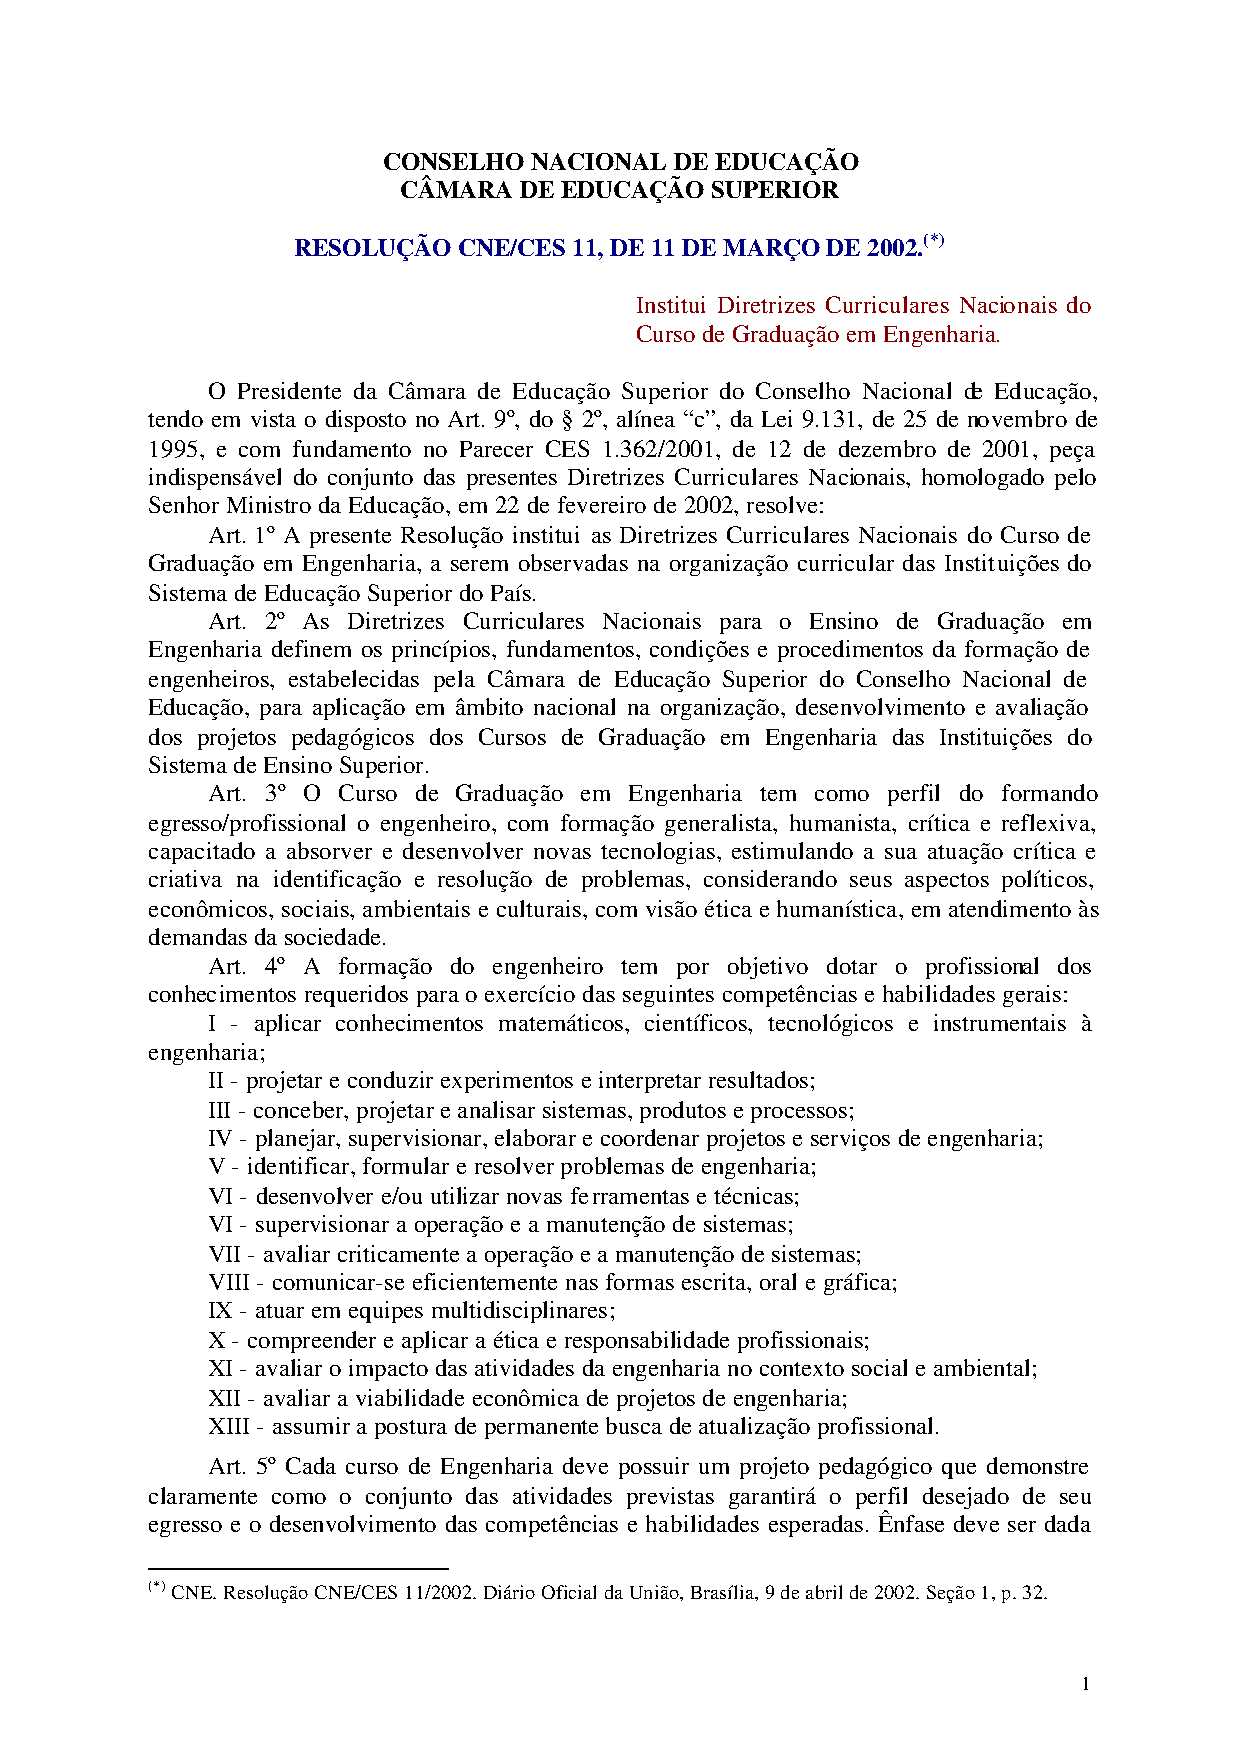
\includepdf[pages=-,pagecommand={\thispagestyle{fancy}}]{leis/CES112002.pdf}
%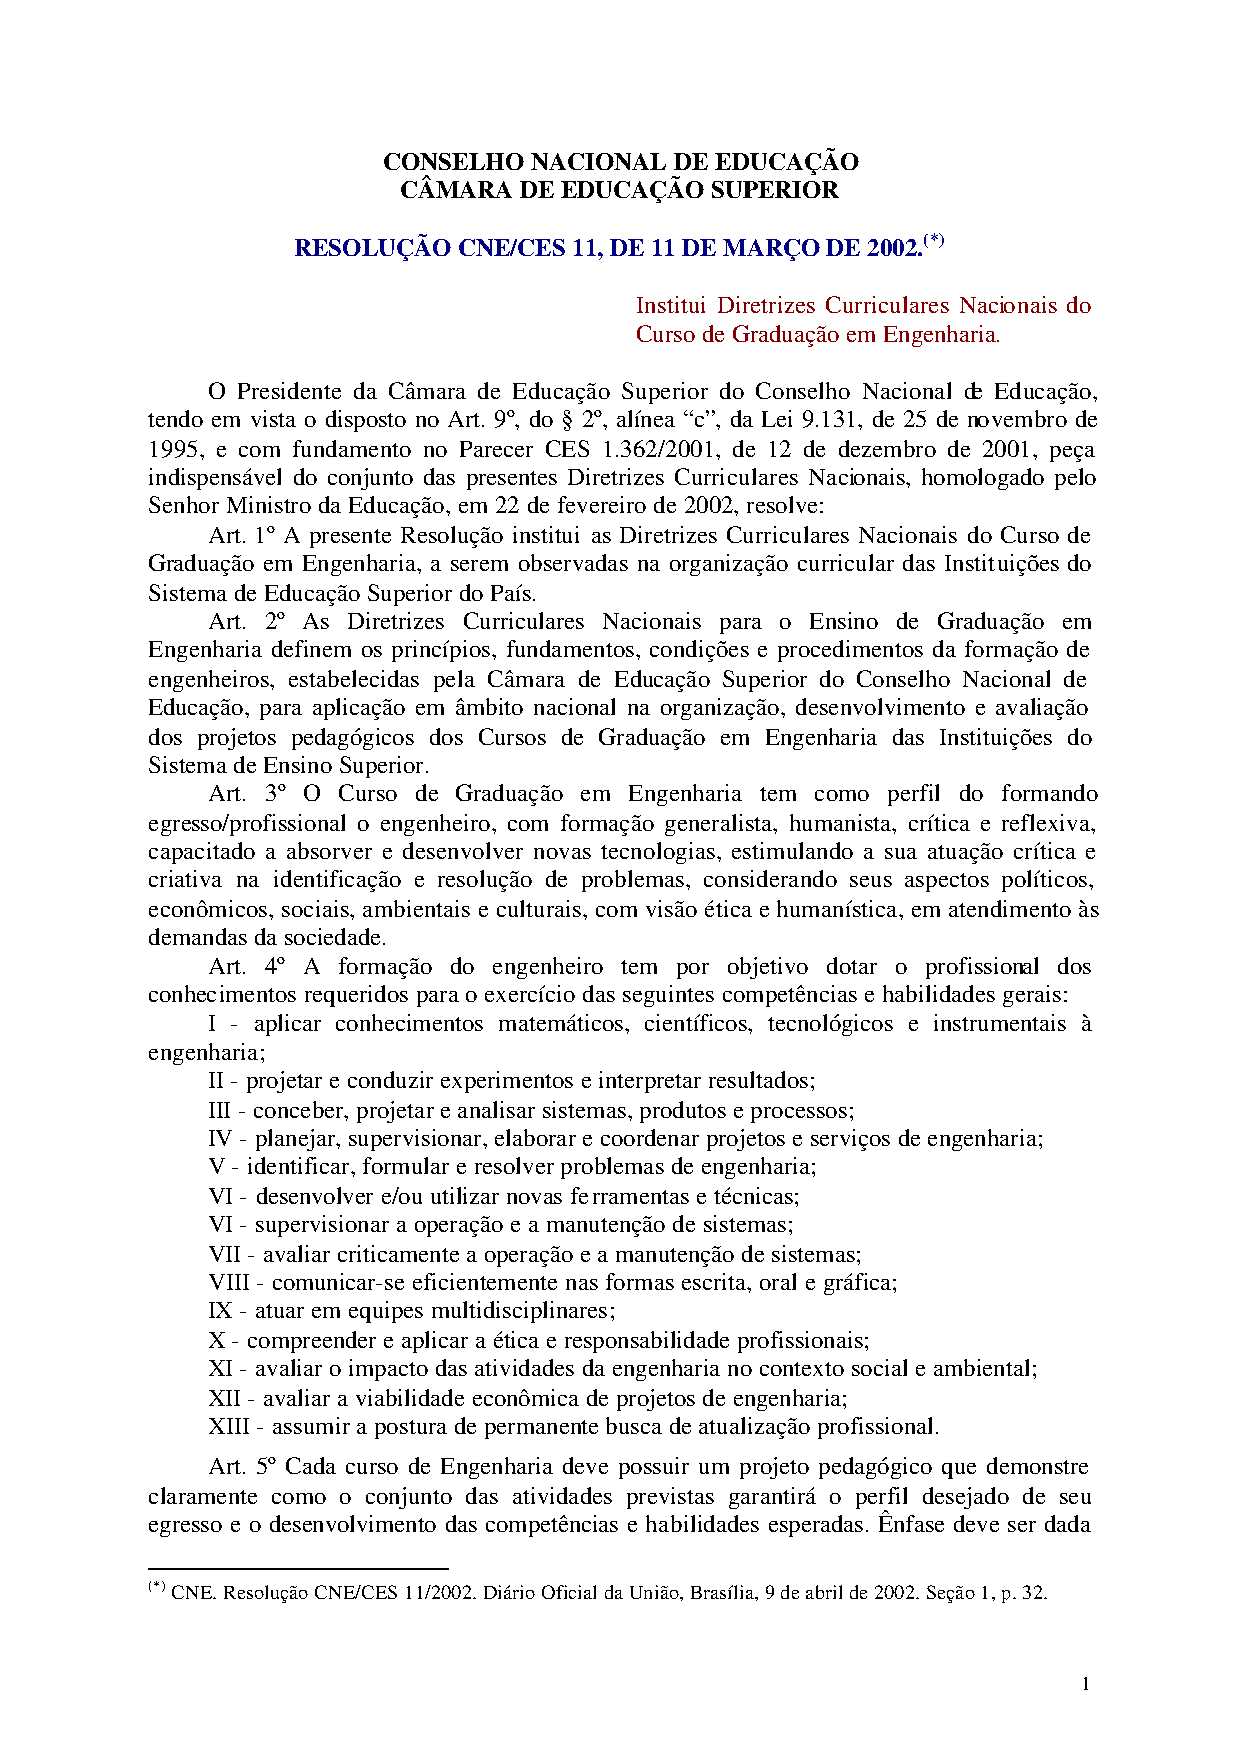
\includepdf[pages=-]{leis/CES112002.pdf}

\chapter{Resolução nº 1.010 CREA/CONFEA}
\label{res1010}
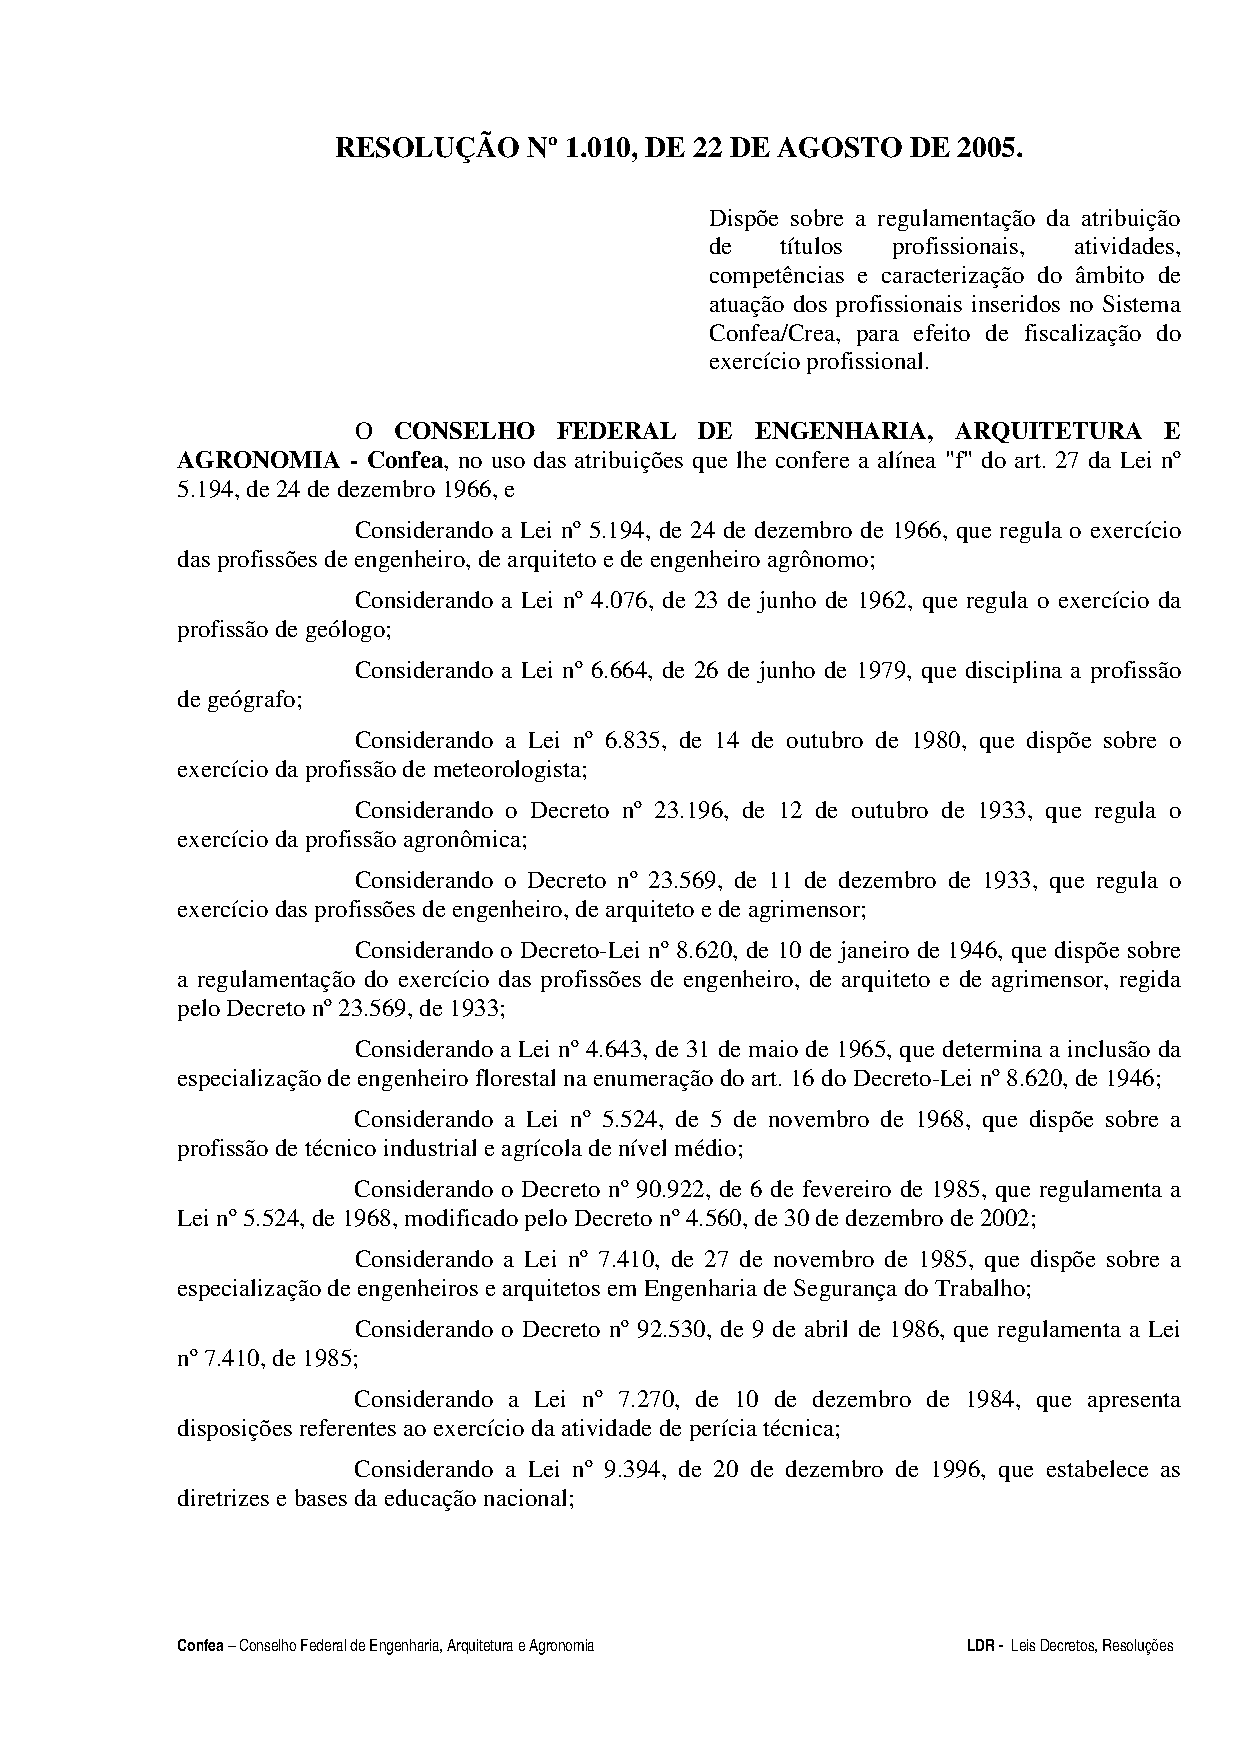
\includepdf[pages=1,pagecommand={\thispagestyle{fancy}}]{leis/res1010.pdf}
\includepdf[pages=2, offset=1.8cm 0,pagecommand={\thispagestyle{fancy}}]{leis/res1010.pdf}
\includepdf[pages=3,pagecommand={\thispagestyle{fancy}}]{leis/res1010.pdf}
\includepdf[pages=4, offset=1.8cm 0,pagecommand={\thispagestyle{fancy}}]{leis/res1010.pdf}
\includepdf[pages=5,pagecommand={\thispagestyle{fancy}}]{leis/res1010.pdf}
\includepdf[pages=6, offset=1.8cm 0,pagecommand={\thispagestyle{fancy}}]{leis/res1010.pdf}
\includepdf[pages=7,pagecommand={\thispagestyle{fancy}}]{leis/res1010.pdf}

\chapter{Fluxograma do Curso de Engenharia de Computação}
\label{fluxograma}
\includepdf[pages=-,angle=90]{pdf/fluxogramaEngenhariaComputacao.pdf}
\chapter{Ementas do Curso de Engenharia de Computação}
\label{ementas}
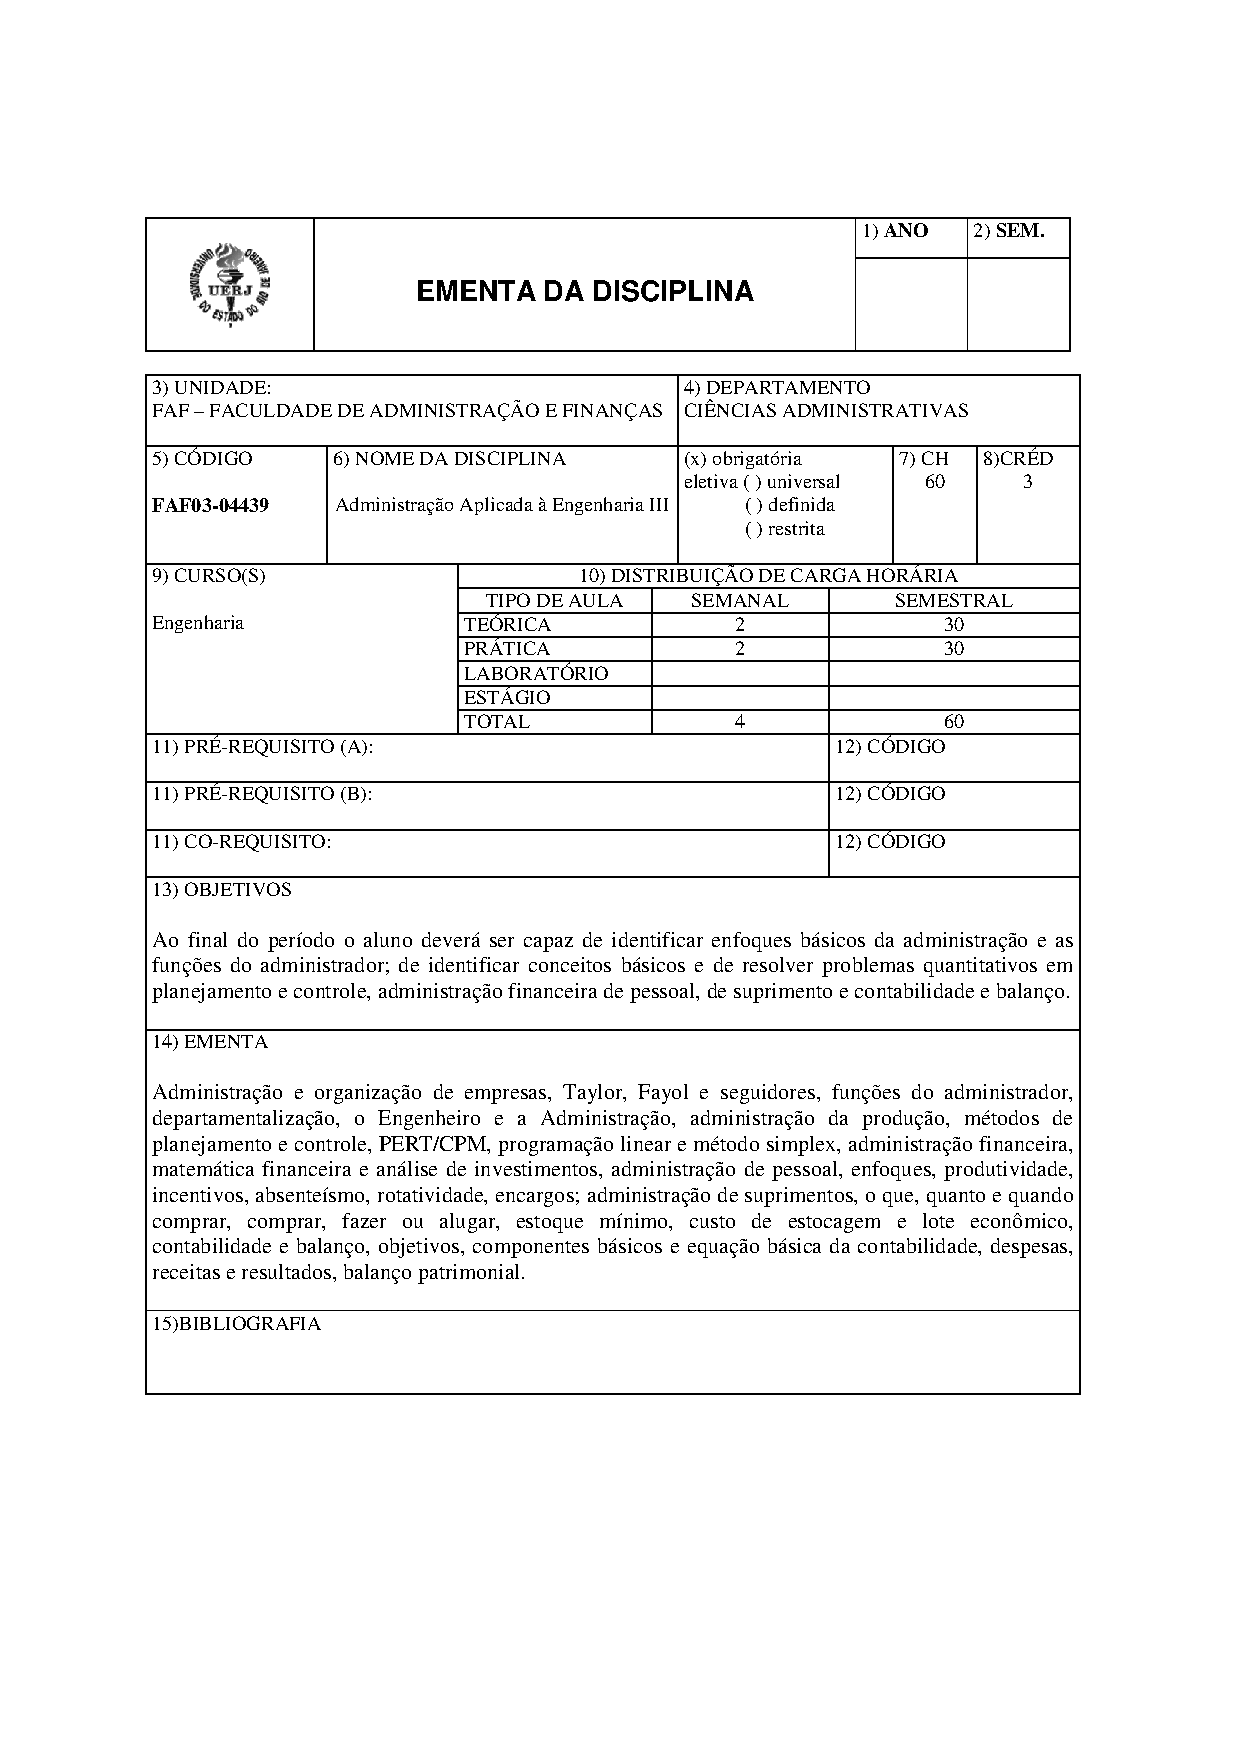
\includepdf[pages=-,addtotoc={1,section,1,{\Adm},},pagecommand={\thispagestyle{fancy}}]{ementasExternas/Administracao.pdf}
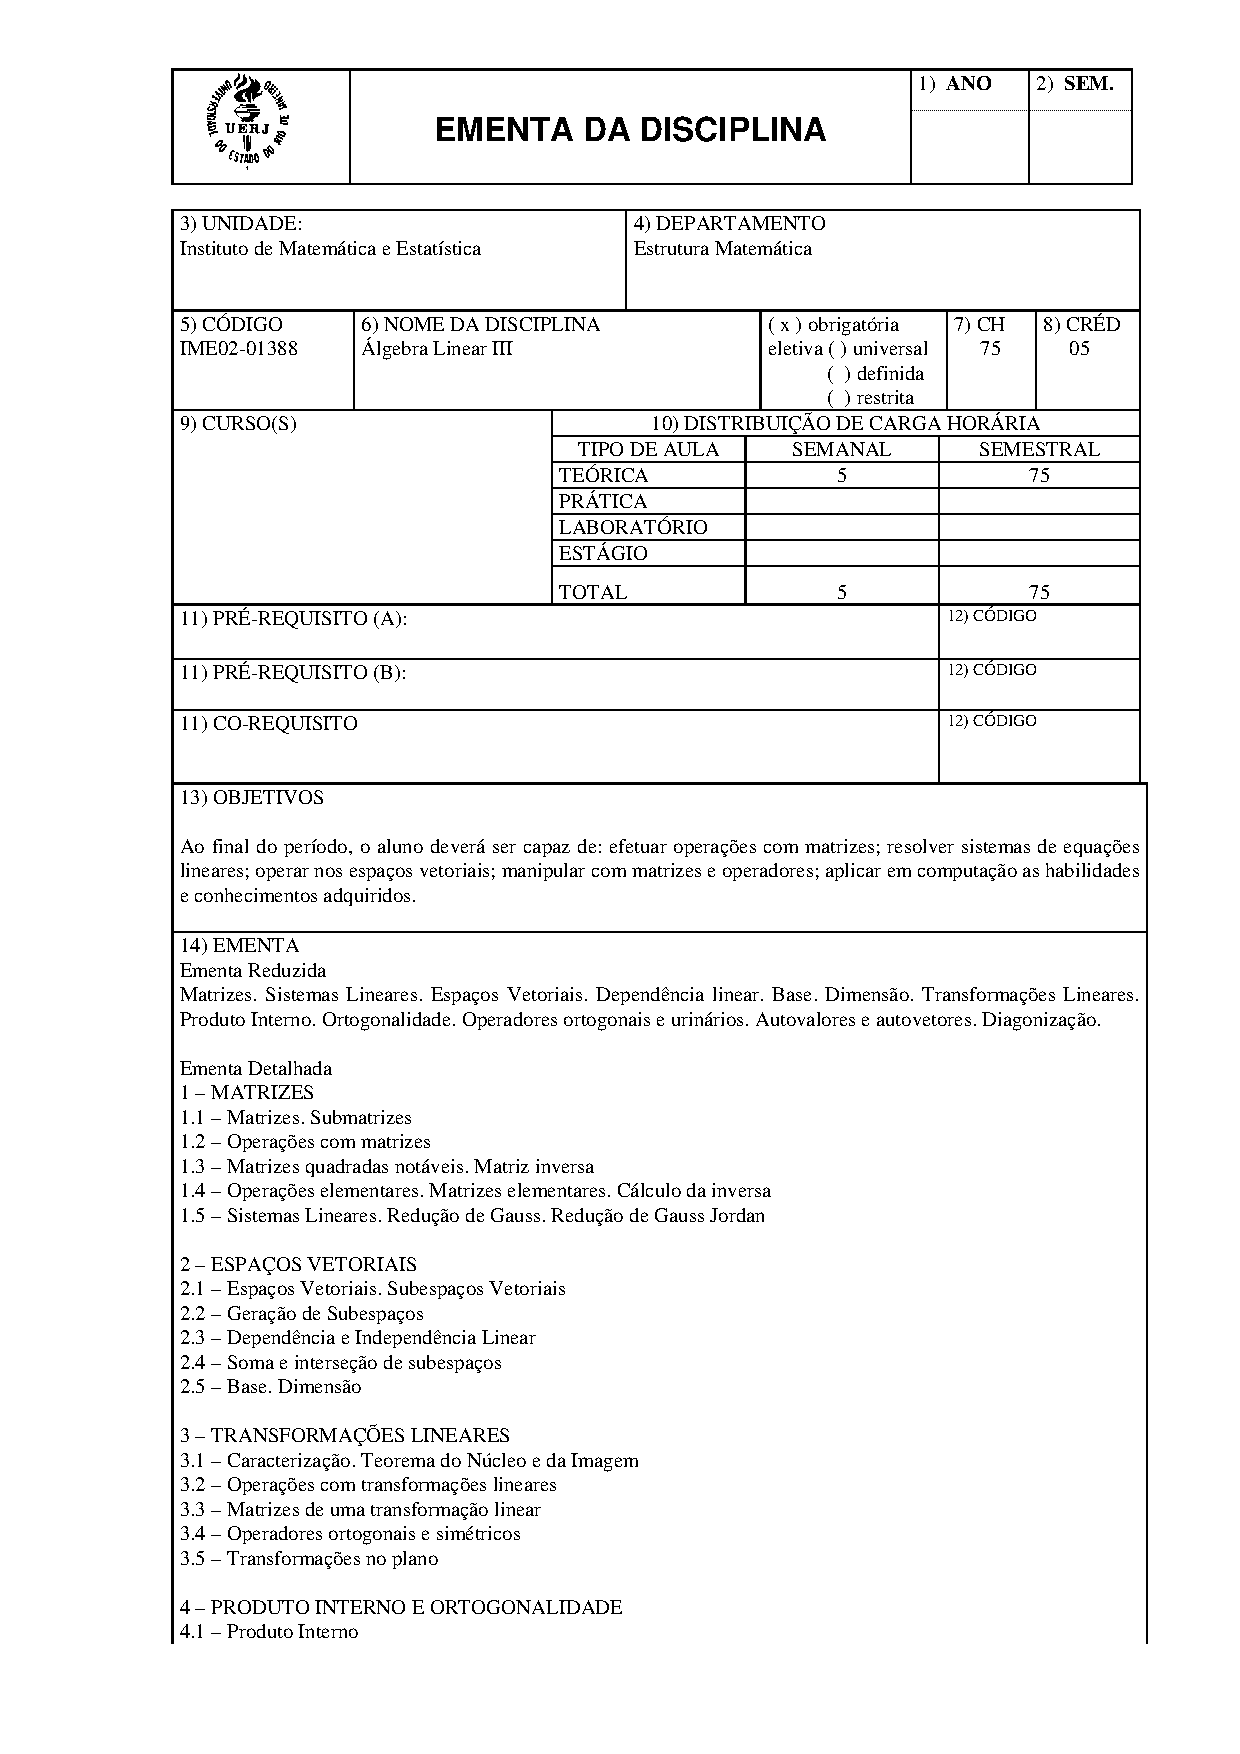
\includepdf[pages=-,addtotoc={1,section,1,{\AlgLin},},pagecommand={\thispagestyle{fancy}}]{ementasExternas/AlgebraLinearIII.pdf}
\includepdf[pages=-,addtotoc={1,section,1,{\AlgComp},},pagecommand={\thispagestyle{fancy}}]{pdf/AlgoritmosComputacionais.pdf}
\includepdf[pages=-,addtotoc={1,section,1,{\AnAlg},},pagecommand={\thispagestyle{fancy}}]{pdf/AnaliseDeAlgoritmos.pdf}
\includepdf[pages=-,addtotoc={1,section,1,{\AnaFis},},pagecommand={\thispagestyle{fancy}}]{pdf/AnaliseDeSistemasFisicos.pdf}

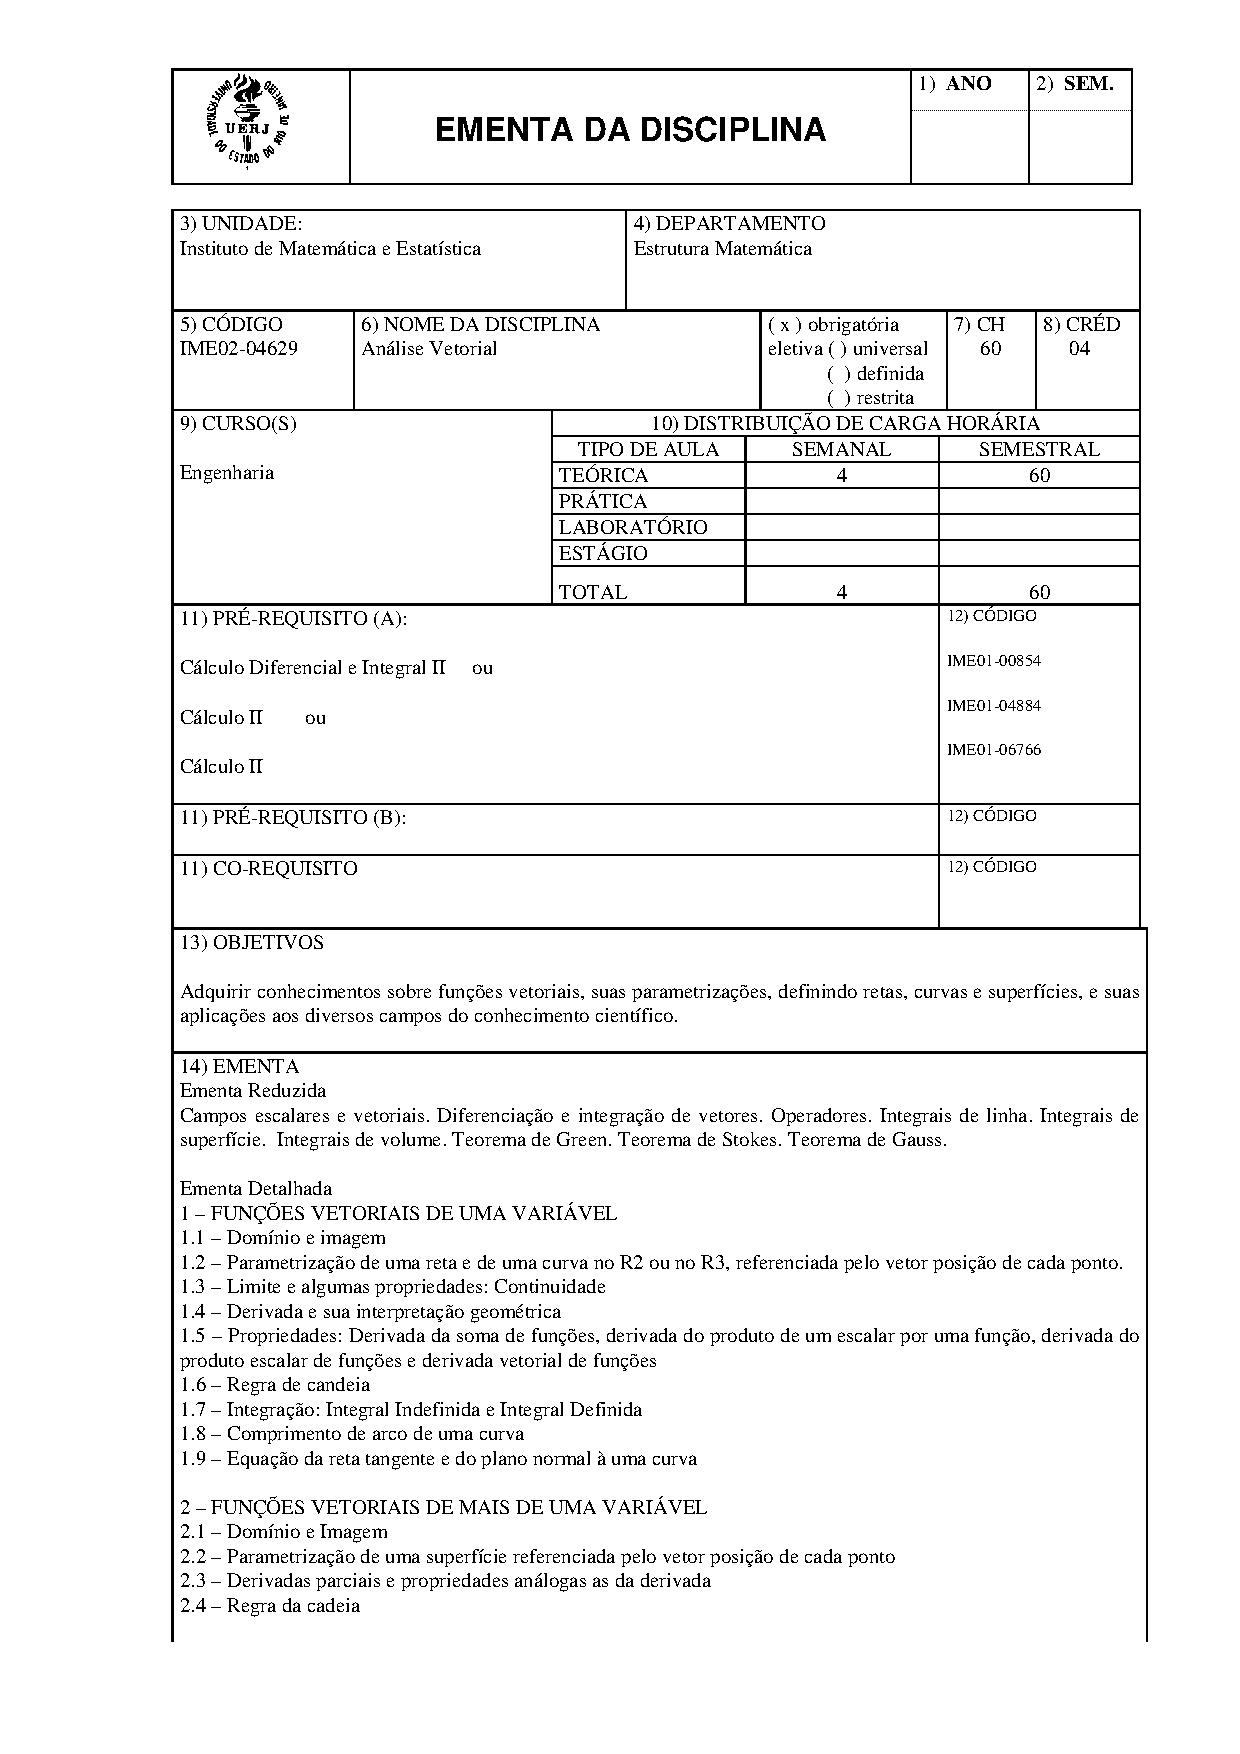
\includepdf[pages=-,addtotoc={1,section,1,{\AnaVet},},pagecommand={\thispagestyle{fancy}}]{ementasExternas/AnaliseVetorial.pdf}
\includepdf[pages=-,addtotoc={1,section,1,{\EletArq},},pagecommand={\thispagestyle{fancy}}]{pdf/Eletiva4_ComputacaoDeAltoDesempenho.pdf}
\includepdf[pages=-,addtotoc={1,section,1,{\ArqComp},},pagecommand={\thispagestyle{fancy}}]{pdf/ArquiteturaDeComputadores.pdf}
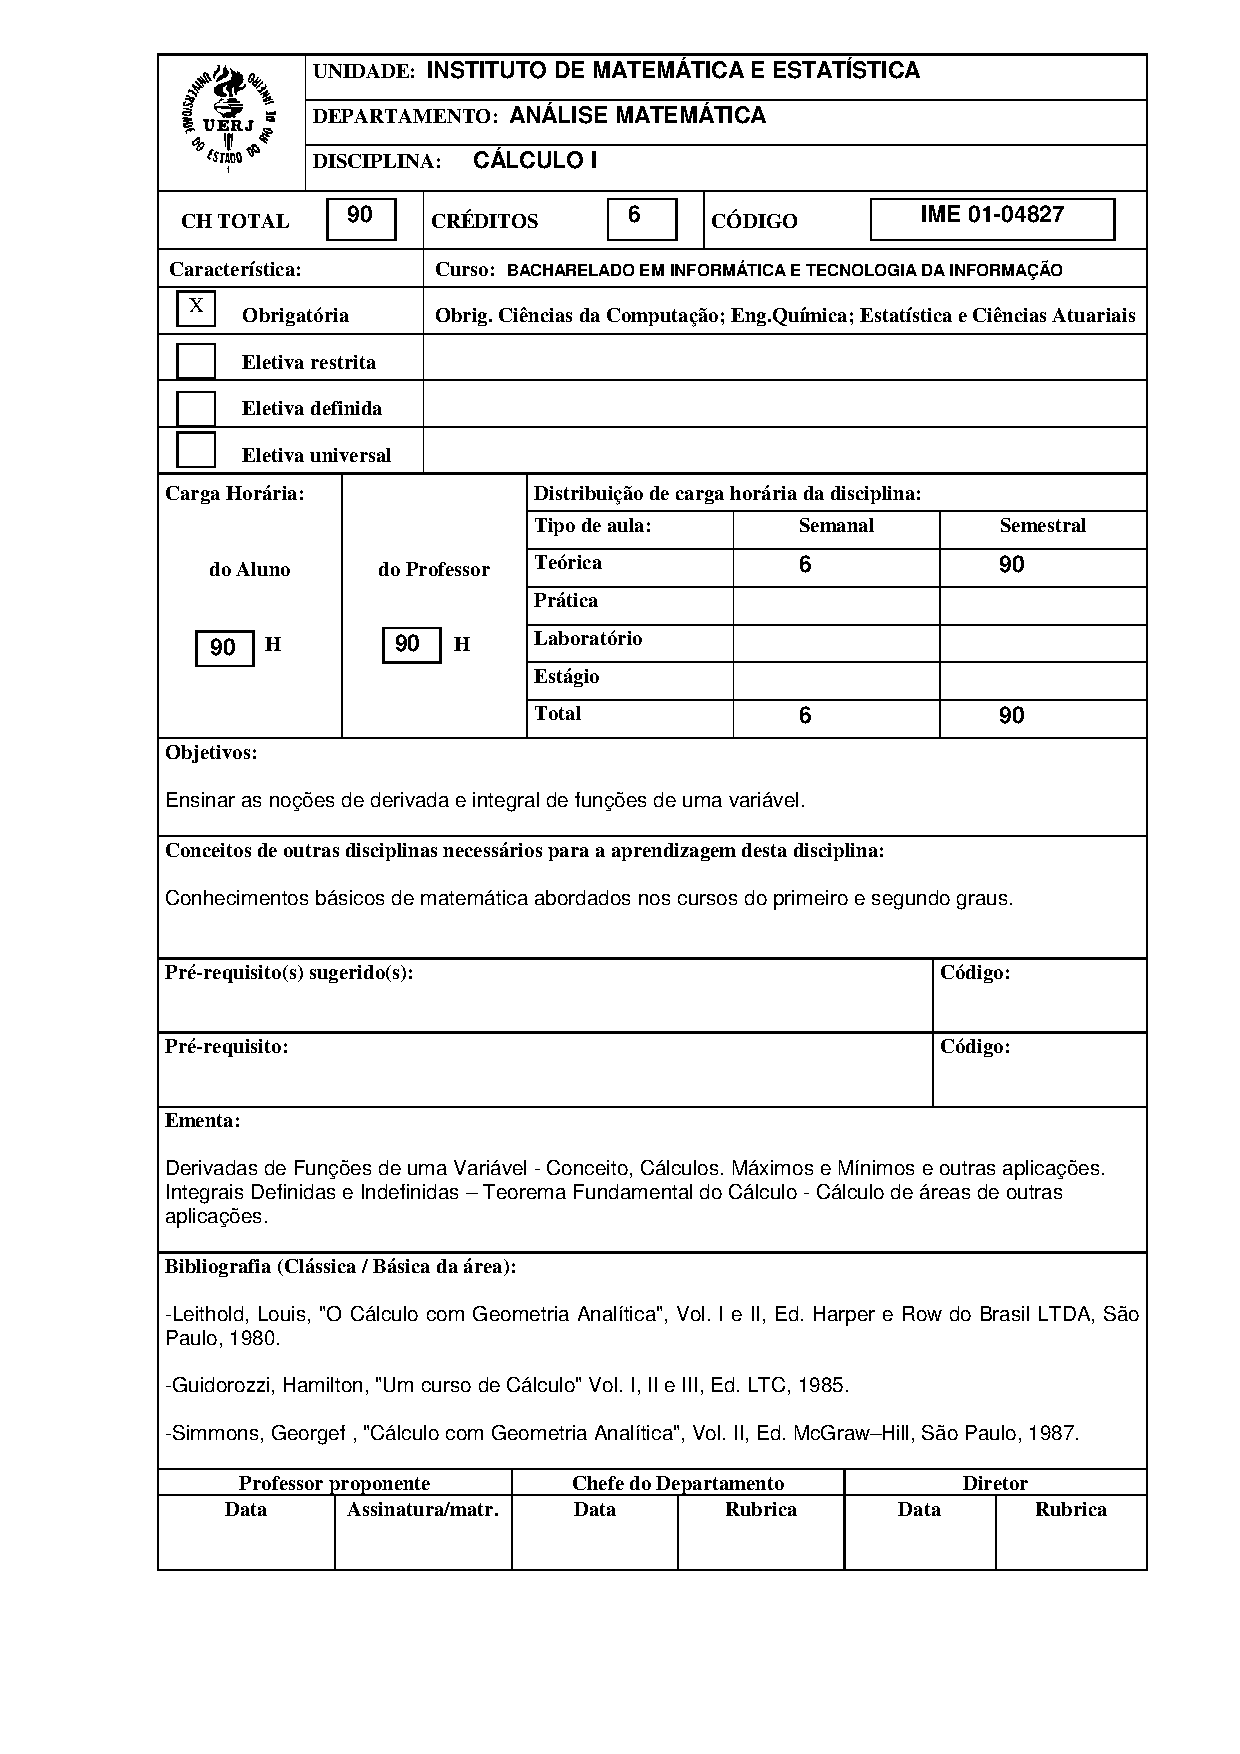
\includepdf[pages=-,addtotoc={1,section,1,{\CalcI},},pagecommand={\thispagestyle{fancy}}]{ementasExternas/CalculoI.pdf}
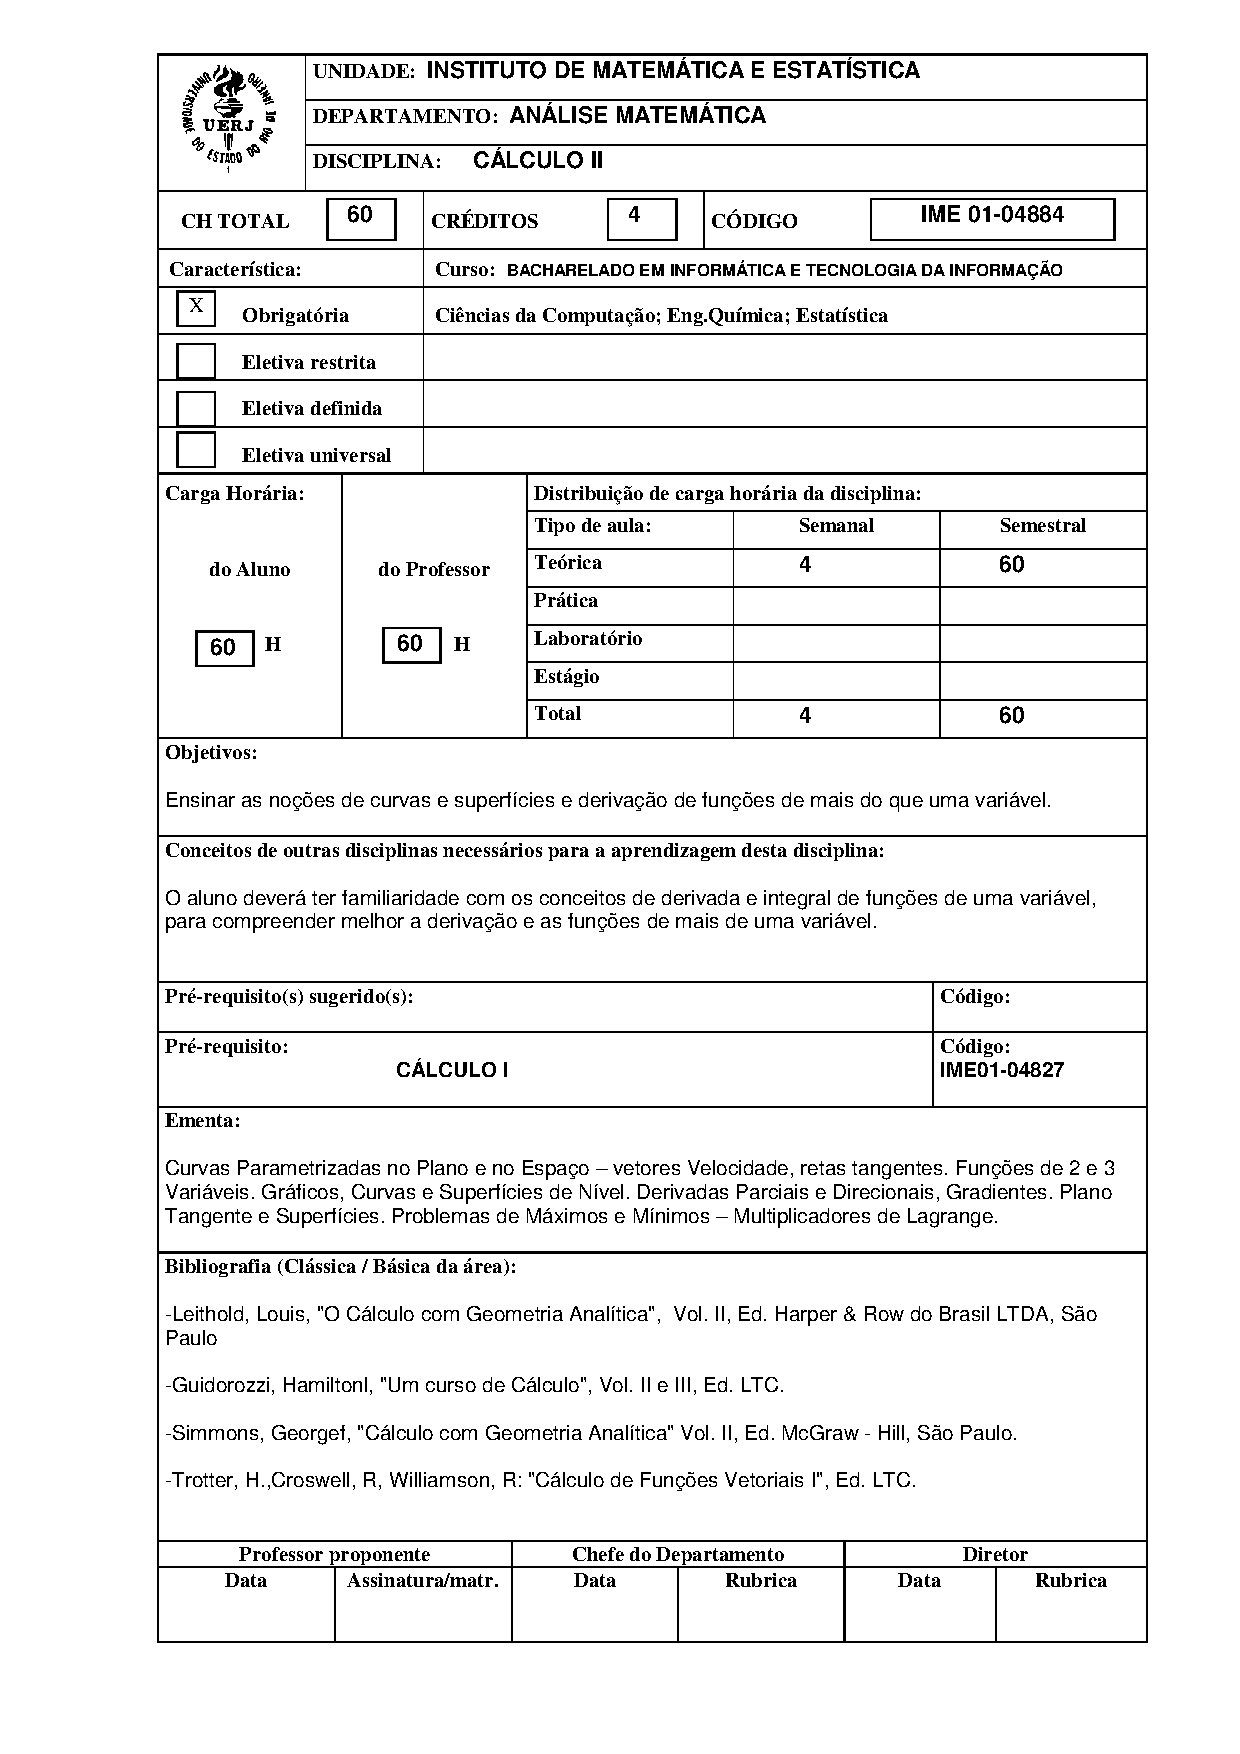
\includepdf[pages=-,addtotoc={1,section,1,{\CalcII},},pagecommand={\thispagestyle{fancy}}]{ementasExternas/CalculoII.pdf}

\includepdf[pages=-,addtotoc={1,section,1,{\CEV},},pagecommand={\thispagestyle{fancy}}]{pdf/CircuitosEletricosV.pdf}
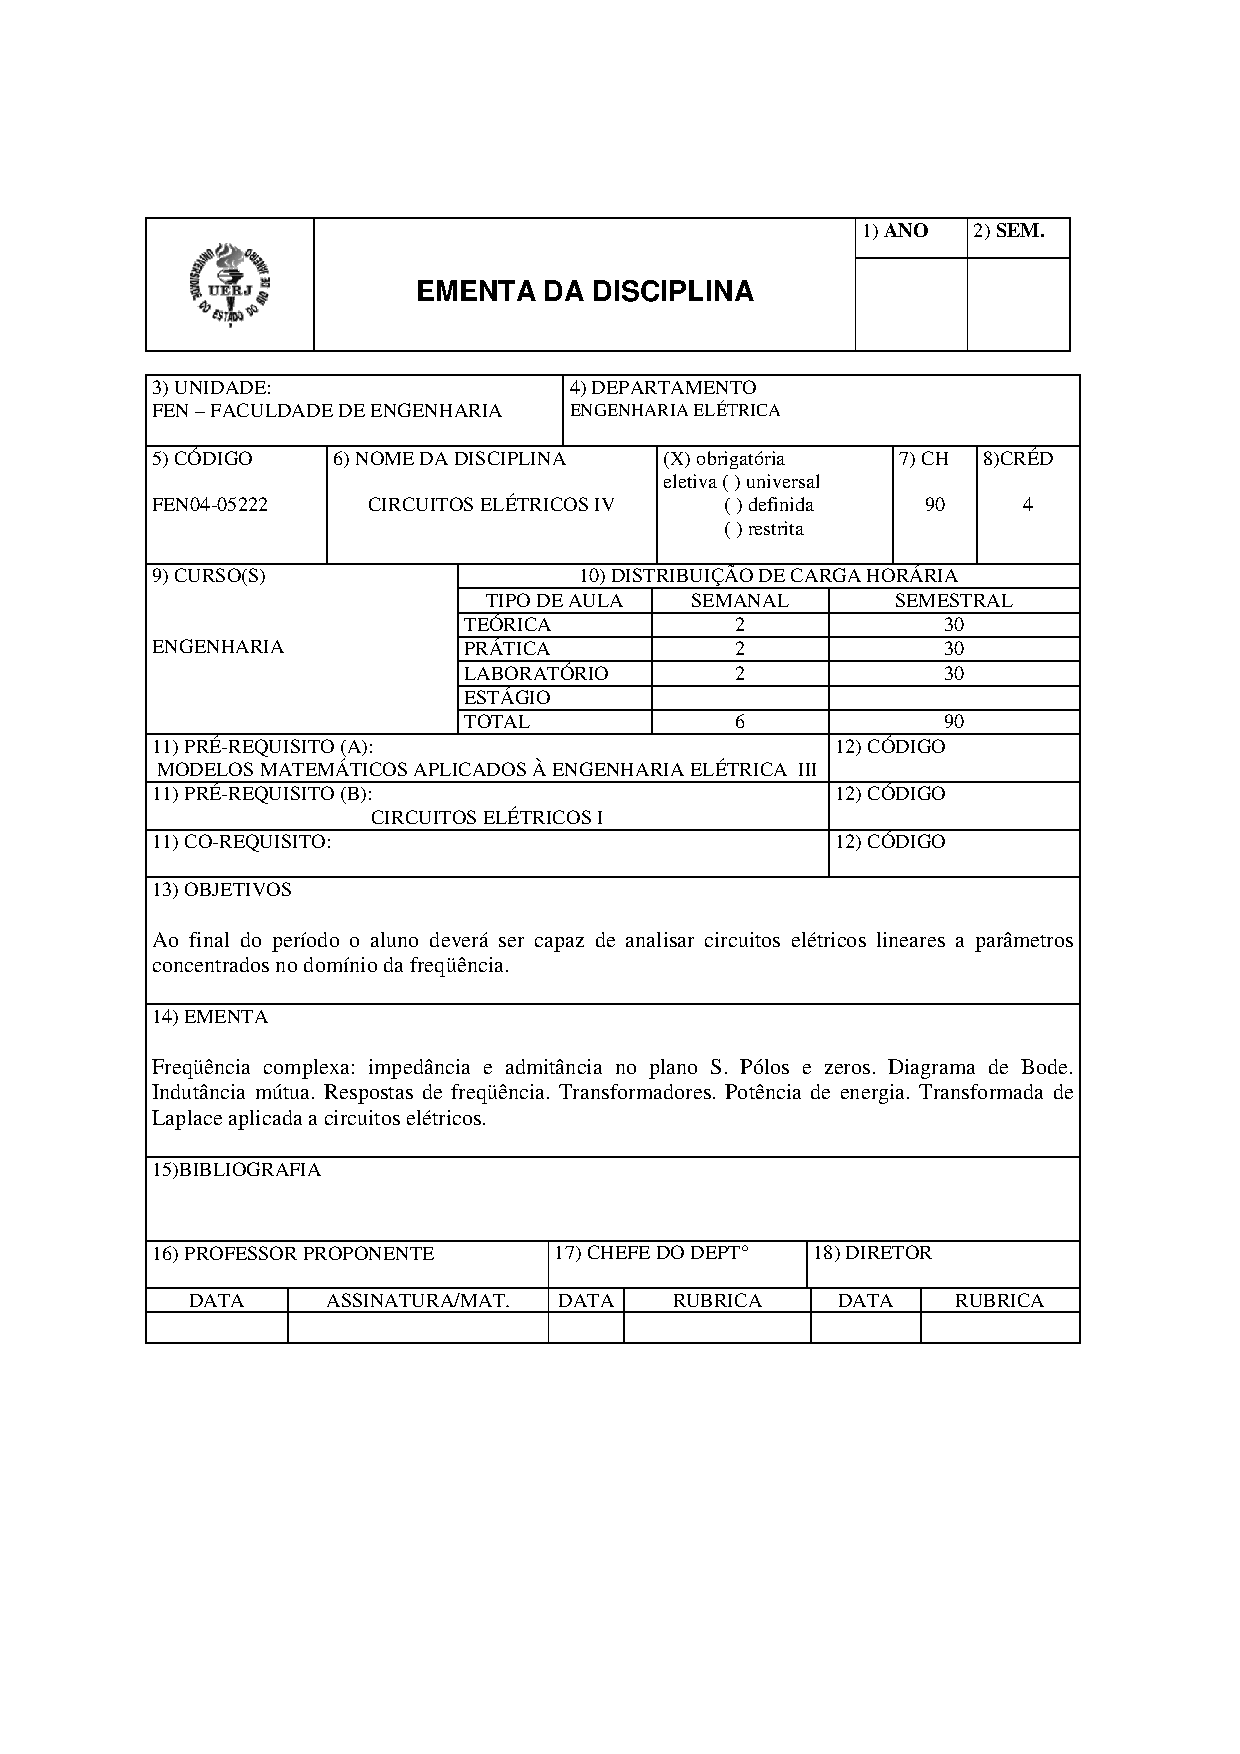
\includepdf[pages=-,addtotoc={1,section,1,{\CEVI},},pagecommand={\thispagestyle{fancy}}]{ementasExternas/CircuitosEletricosIV.pdf}
\includepdf[pages=-,addtotoc={1,section,1,{\CompParal},},pagecommand={\thispagestyle{fancy}}]{pdf/ComputacaoParalela.pdf}
\includepdf[pages=-,addtotoc={1,section,1,{\Control},},pagecommand={\thispagestyle{fancy}}]{pdf/ControleDeProcessosPorComputador.pdf}

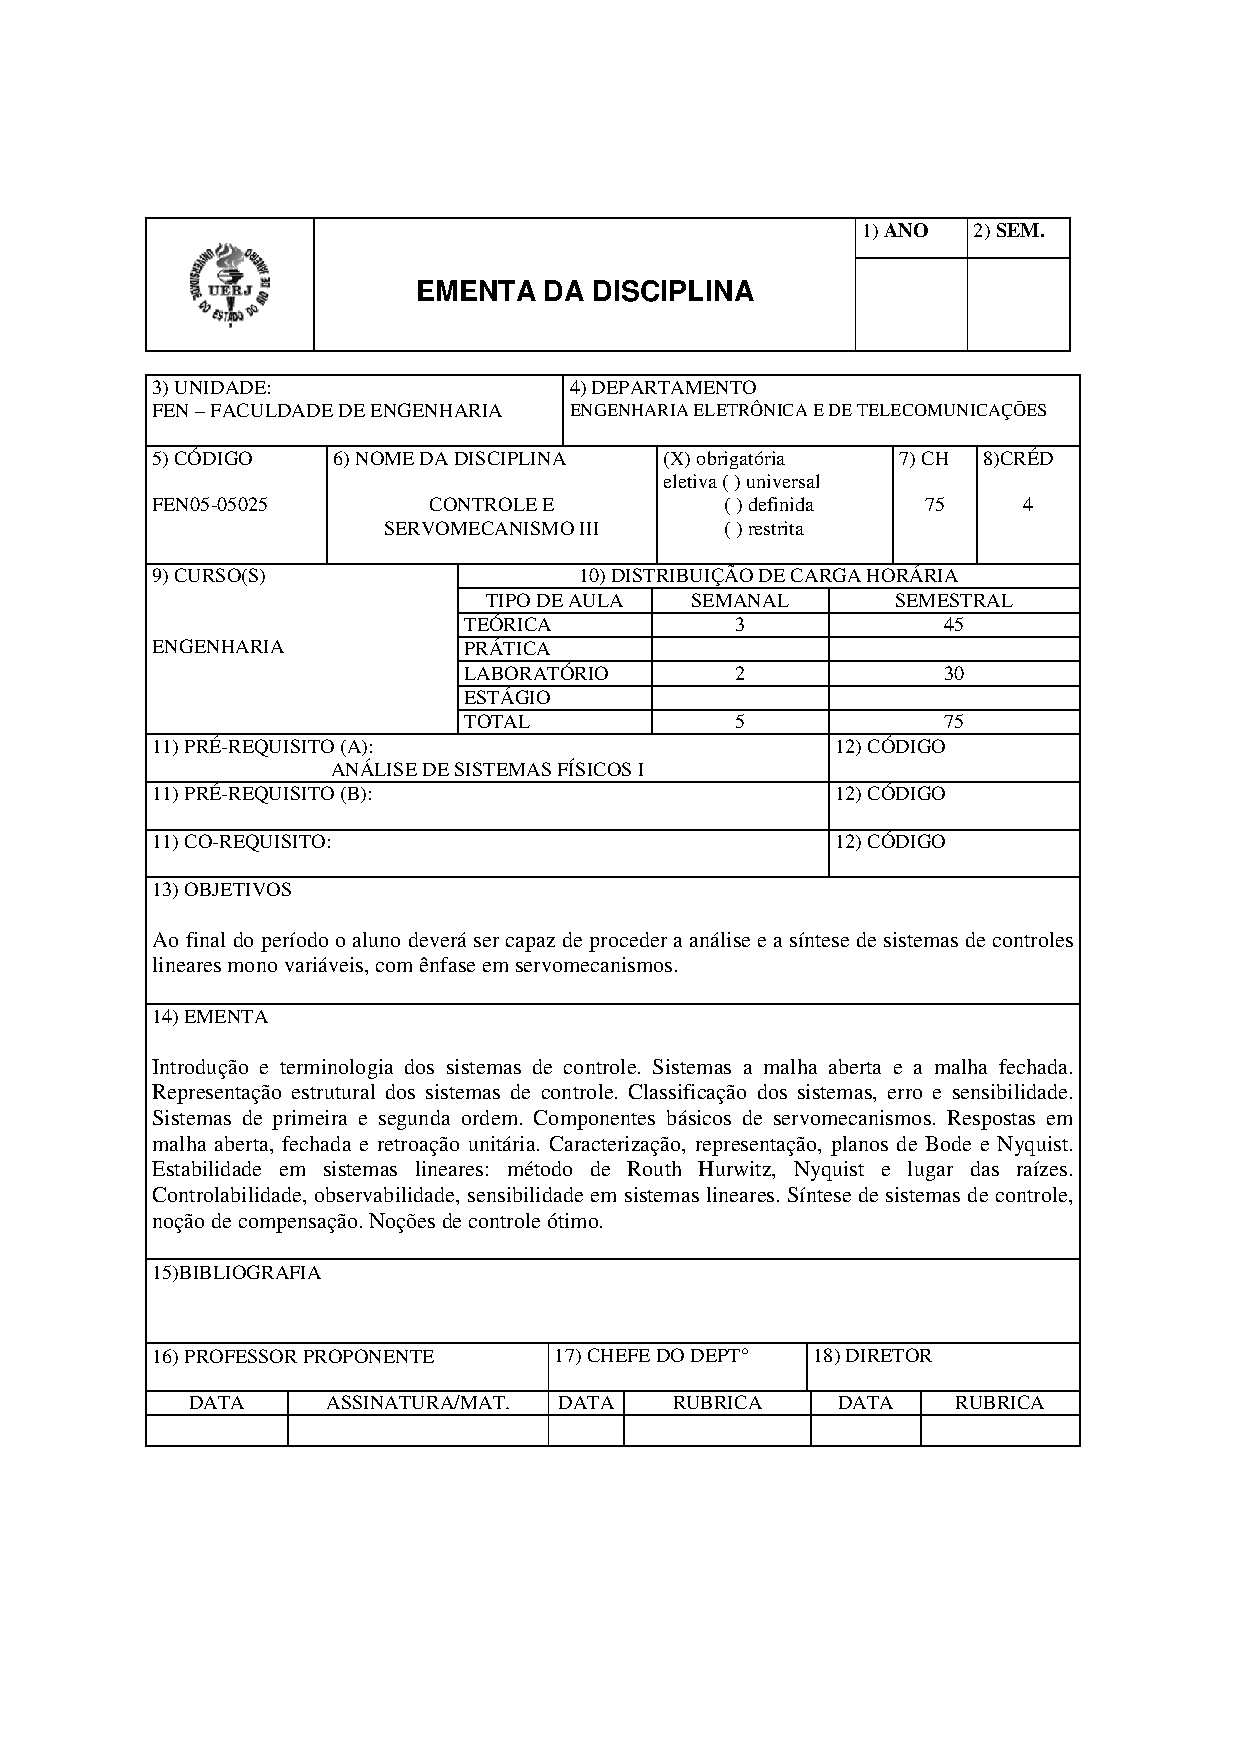
\includepdf[pages=-,addtotoc={1,section,1,{\CServMec},},pagecommand={\thispagestyle{fancy}}]{ementasExternas/ControleEServomecanismosIII.pdf}
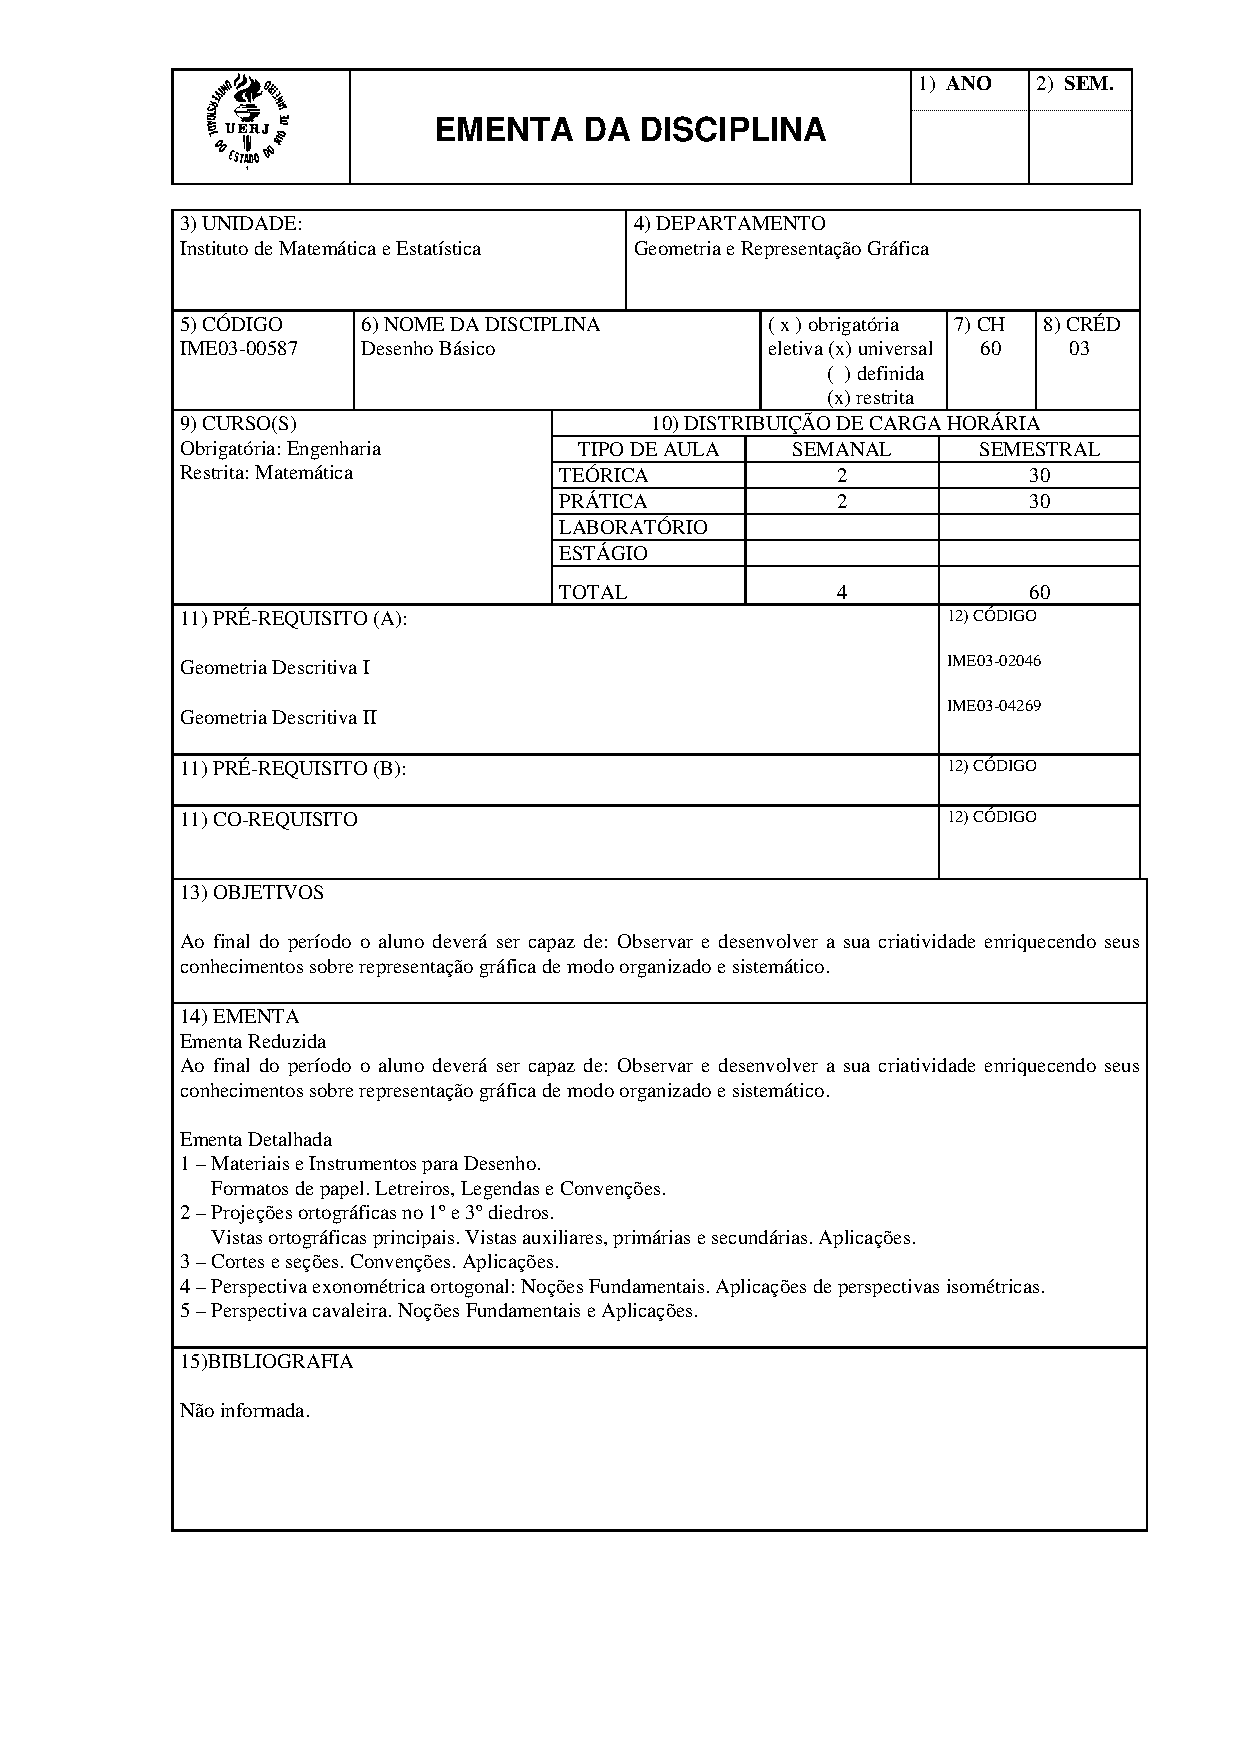
\includepdf[pages=-,addtotoc={1,section,1,{\DesBas},},pagecommand={\thispagestyle{fancy}}]{ementasExternas/DesenhoBasico.pdf}
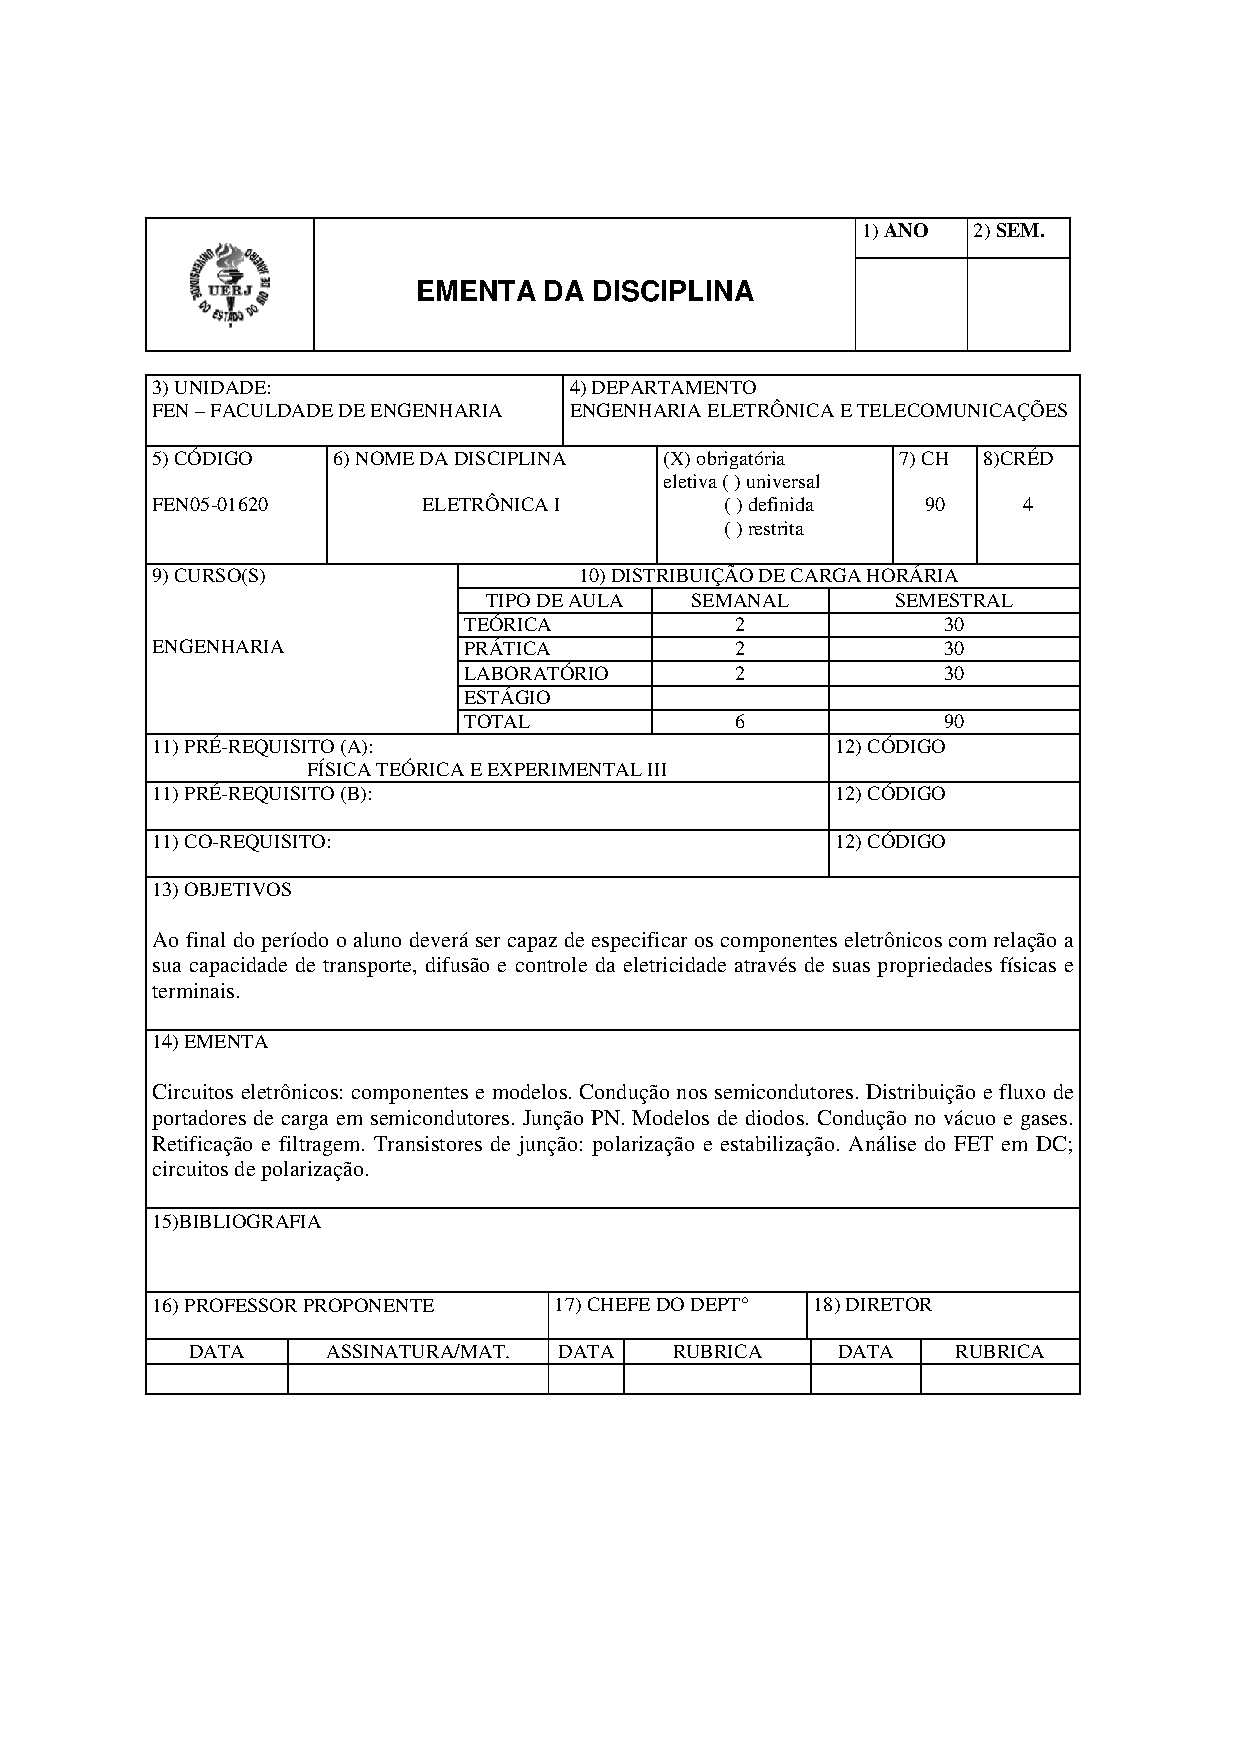
\includepdf[pages=-,addtotoc={1,section,1,{\EletI},},pagecommand={\thispagestyle{fancy}}]{ementasExternas/EletronicaI.pdf}
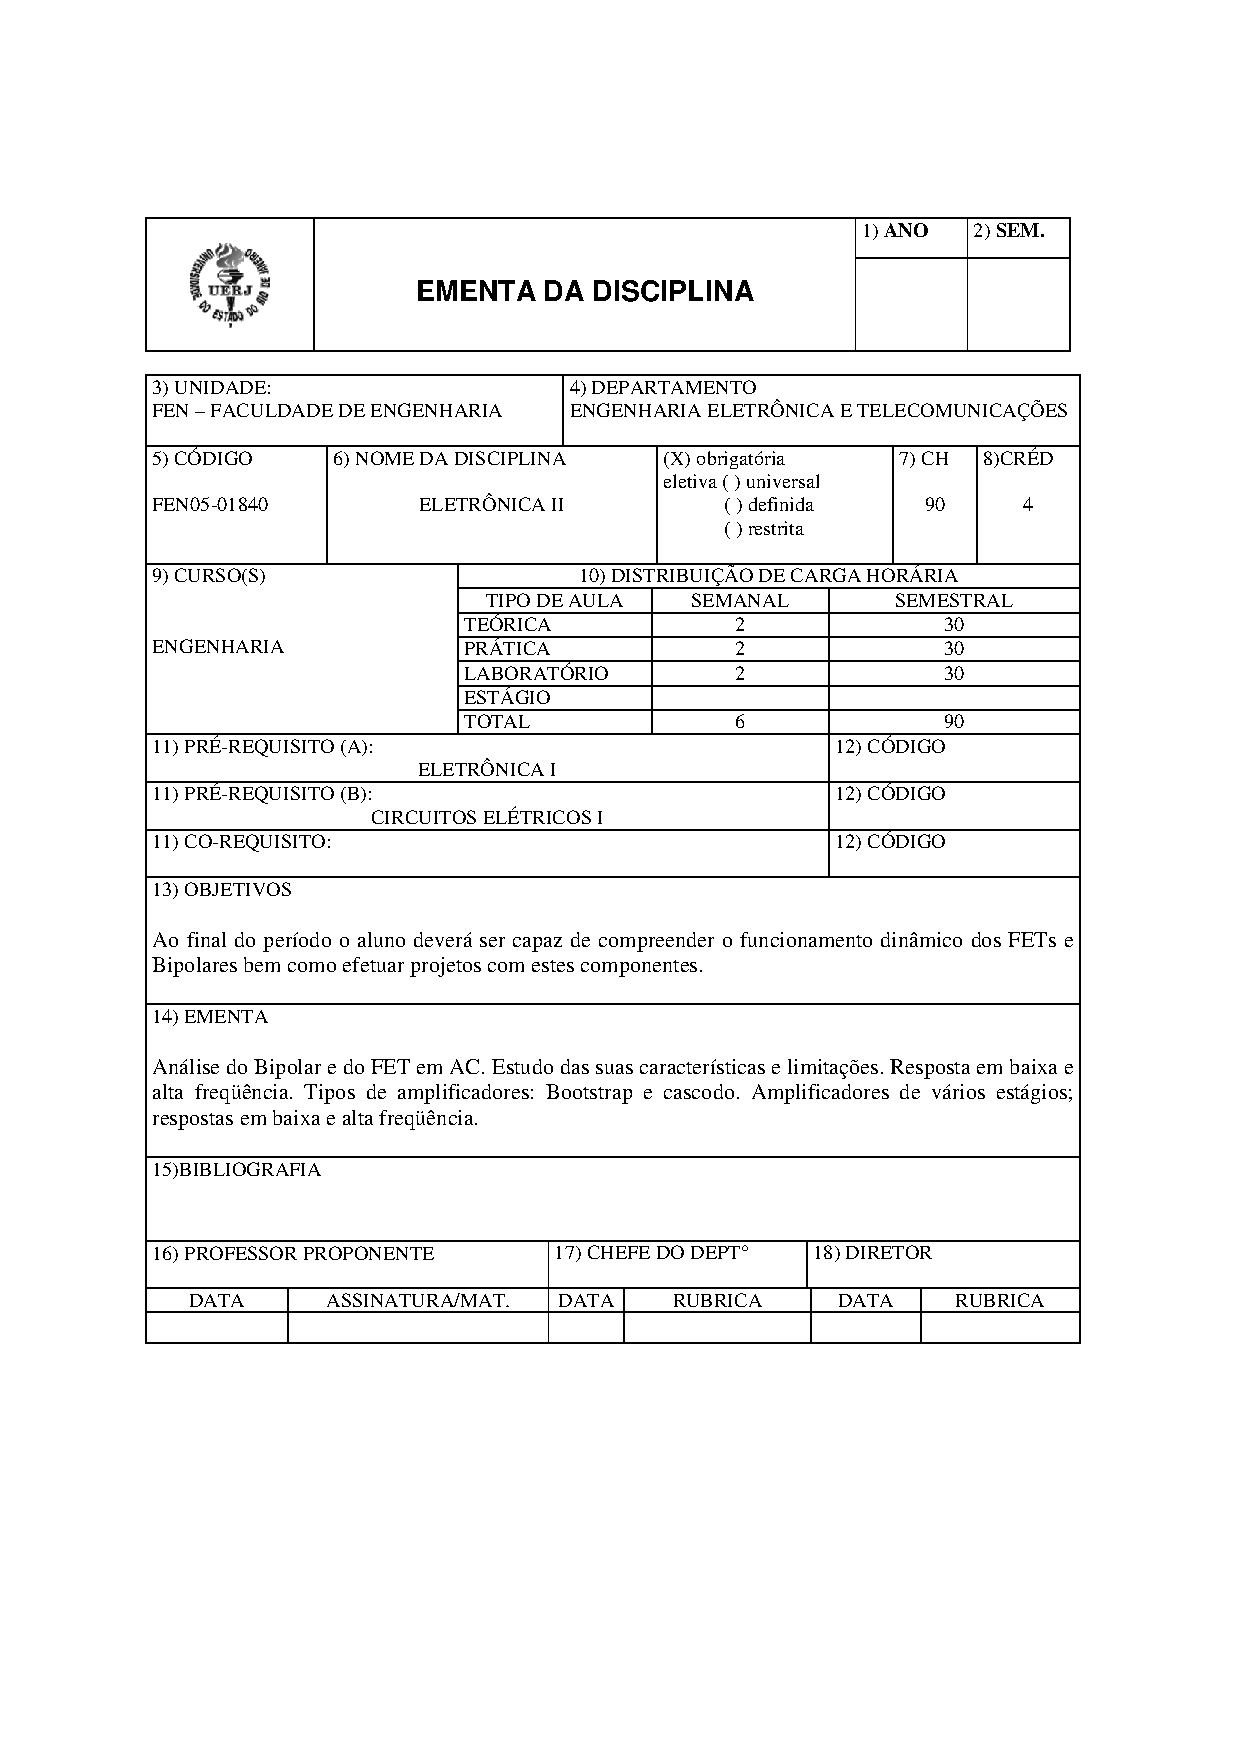
\includepdf[pages=-,addtotoc={1,section,1,{\EletIIA},},pagecommand={\thispagestyle{fancy}}]{ementasExternas/EletronicaII.pdf}
\includepdf[pages=-,addtotoc={1,section,1,{\EngComput},},pagecommand={\thispagestyle{fancy}}]{pdf/EngenhariaComputacional.pdf}

\includepdf[pages=-,addtotoc={1,section,1,{\EngSistA},},pagecommand={\thispagestyle{fancy}}]{pdf/EngenhariaDeSistemas.pdf}
\includepdf[pages=-,addtotoc={1,section,1,{\EngCompSoc},},pagecommand={\thispagestyle{fancy}}]{pdf/EngenhariaDeComputacaoESociedade.pdf}
\includepdf[pages=-,addtotoc={1,section,1,{\SegHig},},pagecommand={\thispagestyle{fancy}}]{pdf/EngenhariaDoTrabalhoI.pdf}
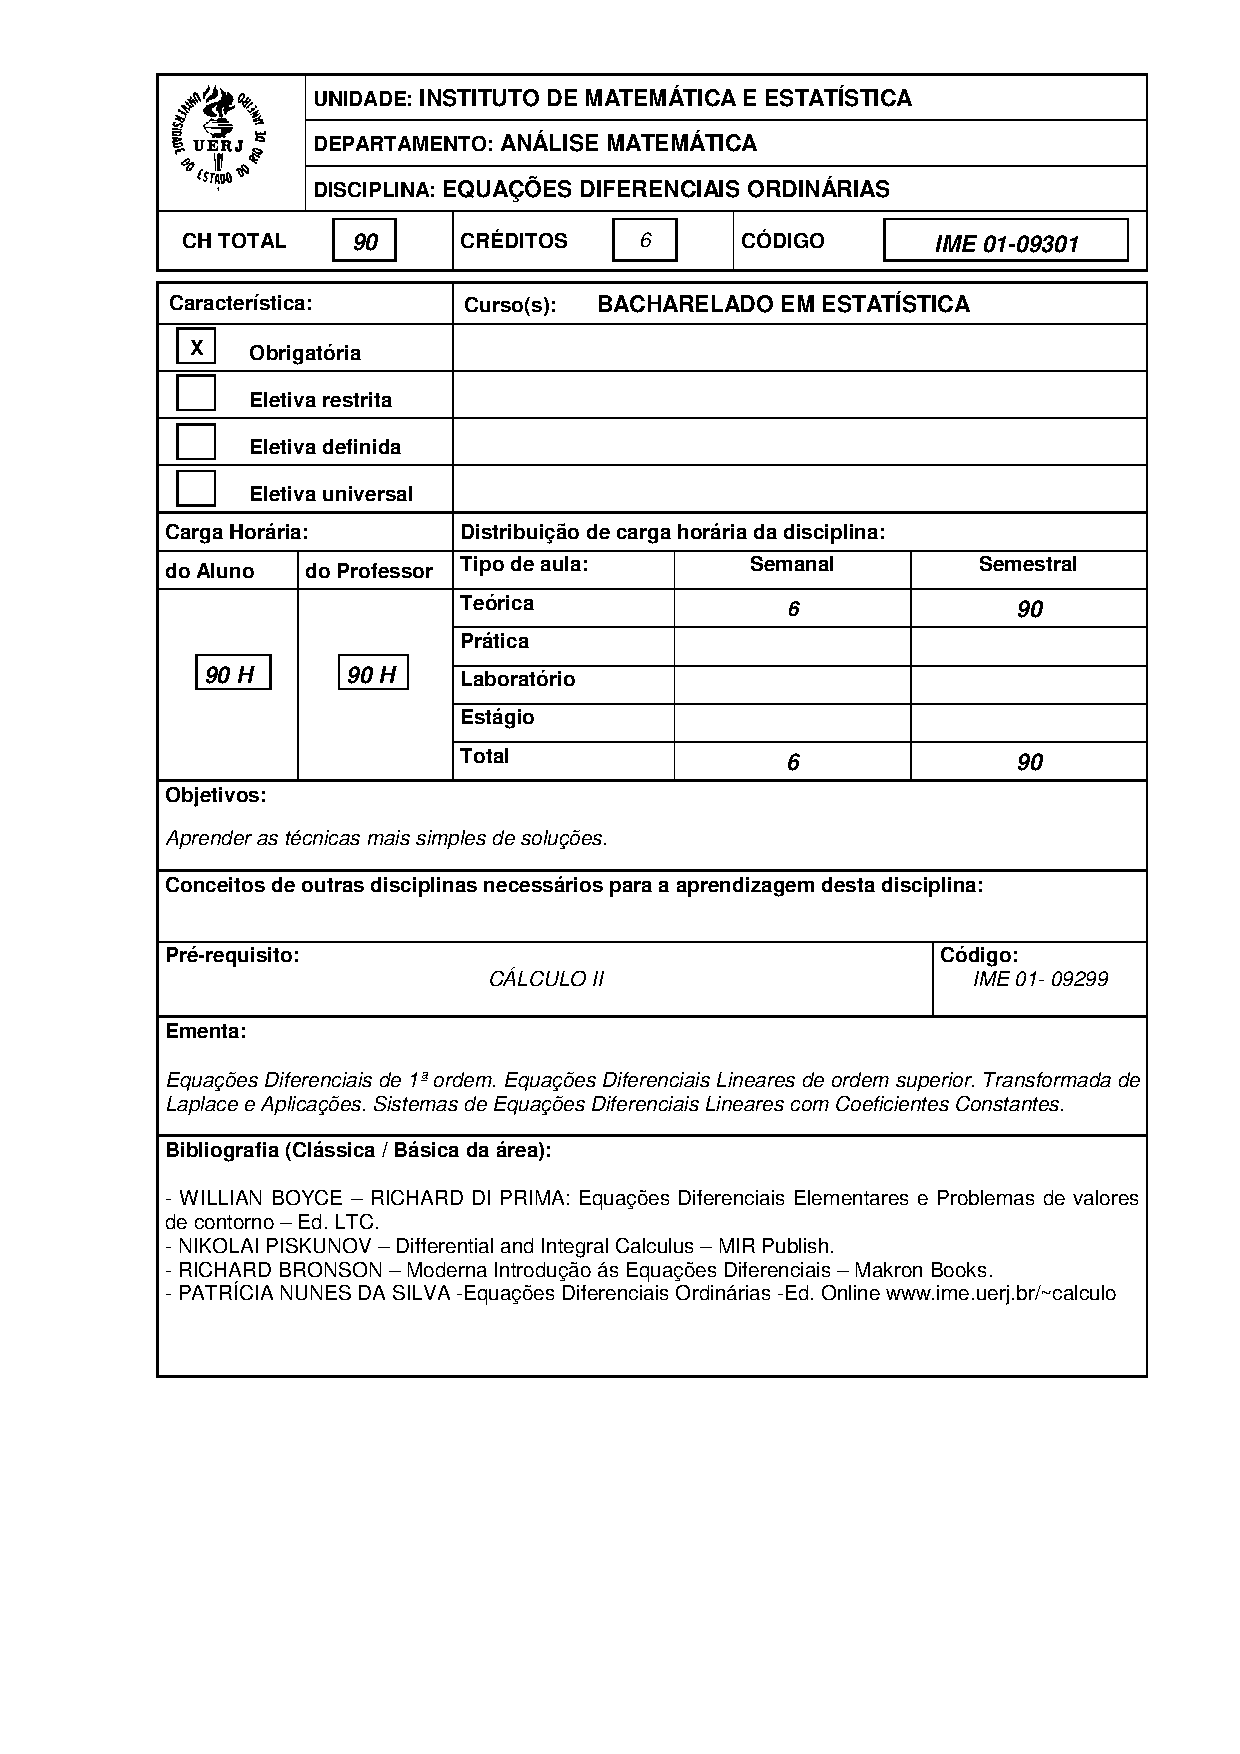
\includepdf[pages=-,addtotoc={1,section,1,{\CalcIII},},pagecommand={\thispagestyle{fancy}}]{ementasExternas/EDO.pdf}
\includepdf[pages=-,addtotoc={1,section,1,{\EstSup},},pagecommand={\thispagestyle{fancy}}]{pdf/EstagioSupervisionadoXIA.pdf}
\includepdf[pages=-,addtotoc={1,section,1,{\EstrInf},},pagecommand={\thispagestyle{fancy}}]{pdf/EstruturasDeInformacao.pdf}

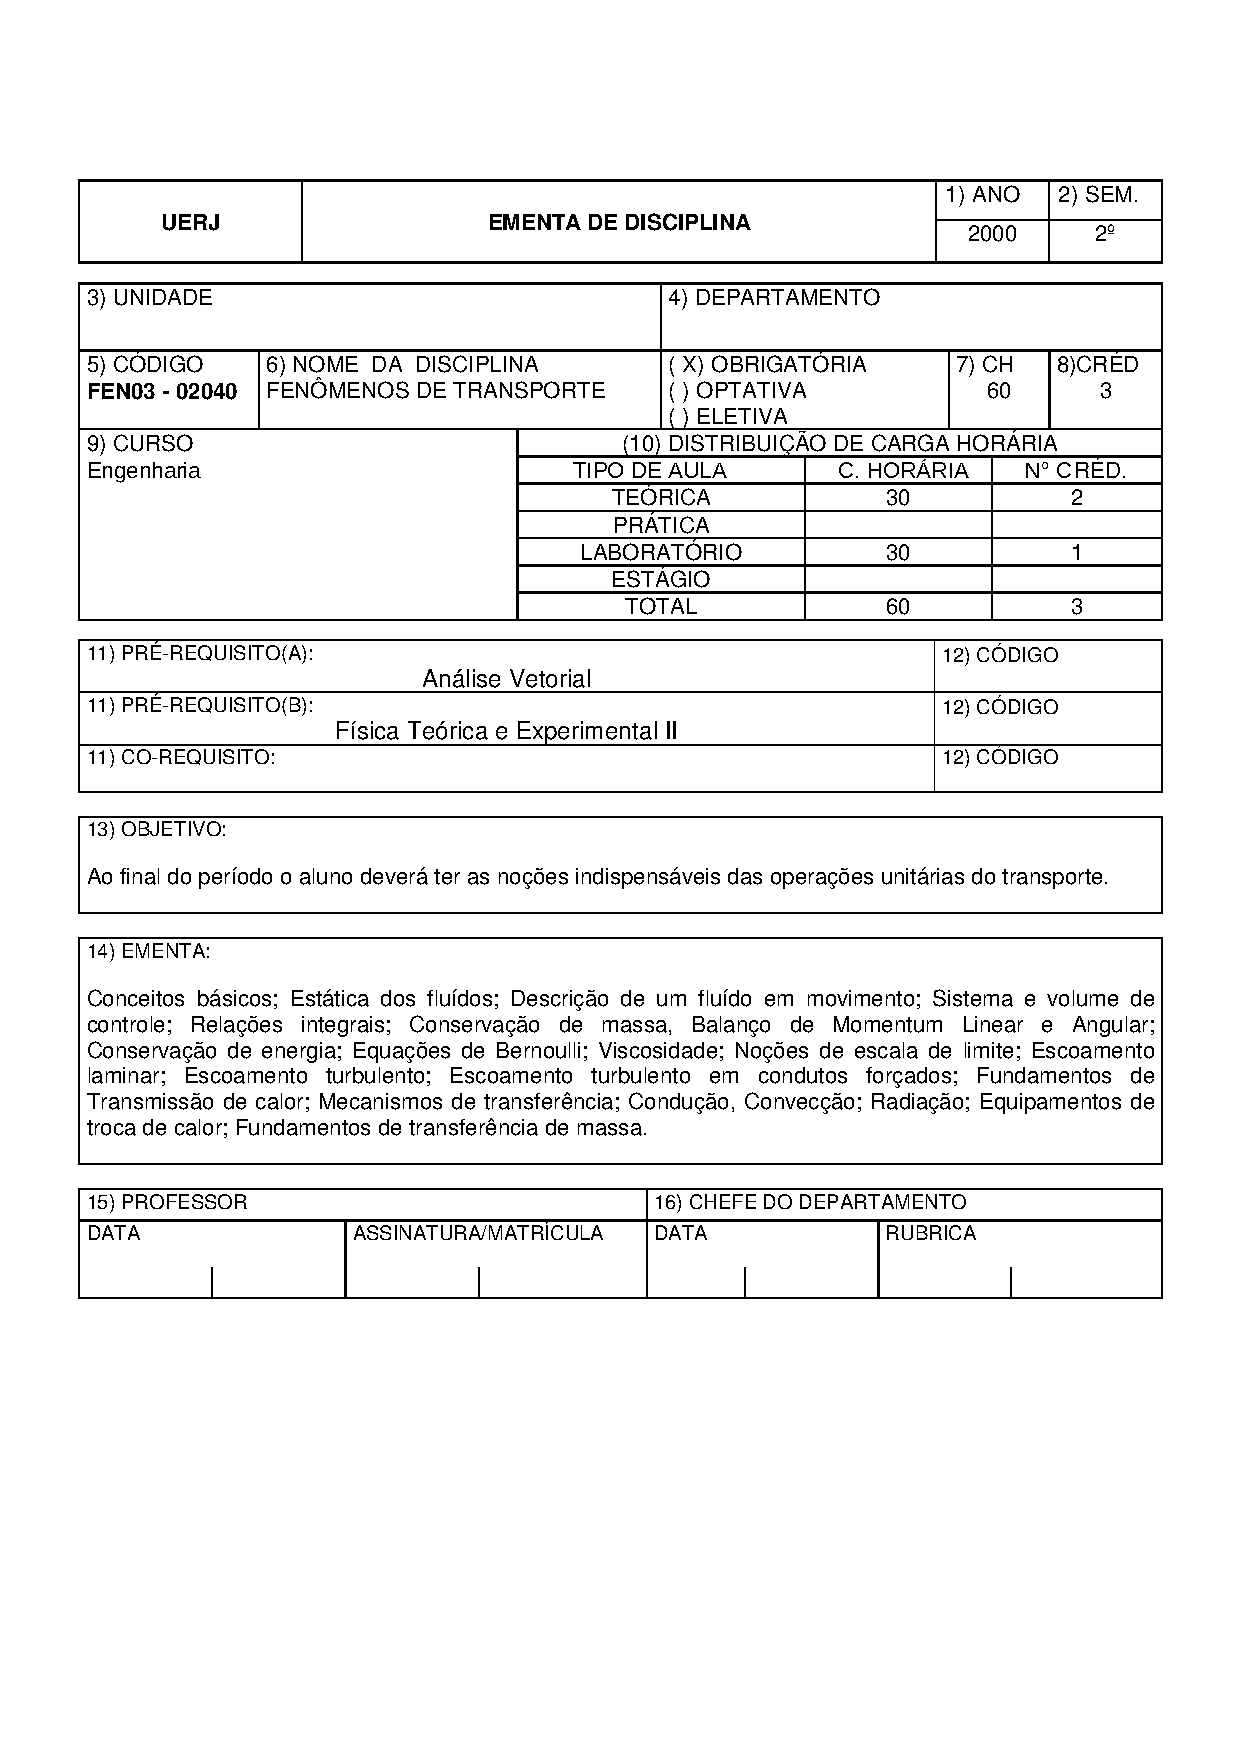
\includepdf[pages=-,addtotoc={1,section,1,{\FenTran},},pagecommand={\thispagestyle{fancy}}]{ementasExternas/FenomenosDeTransporte.pdf}
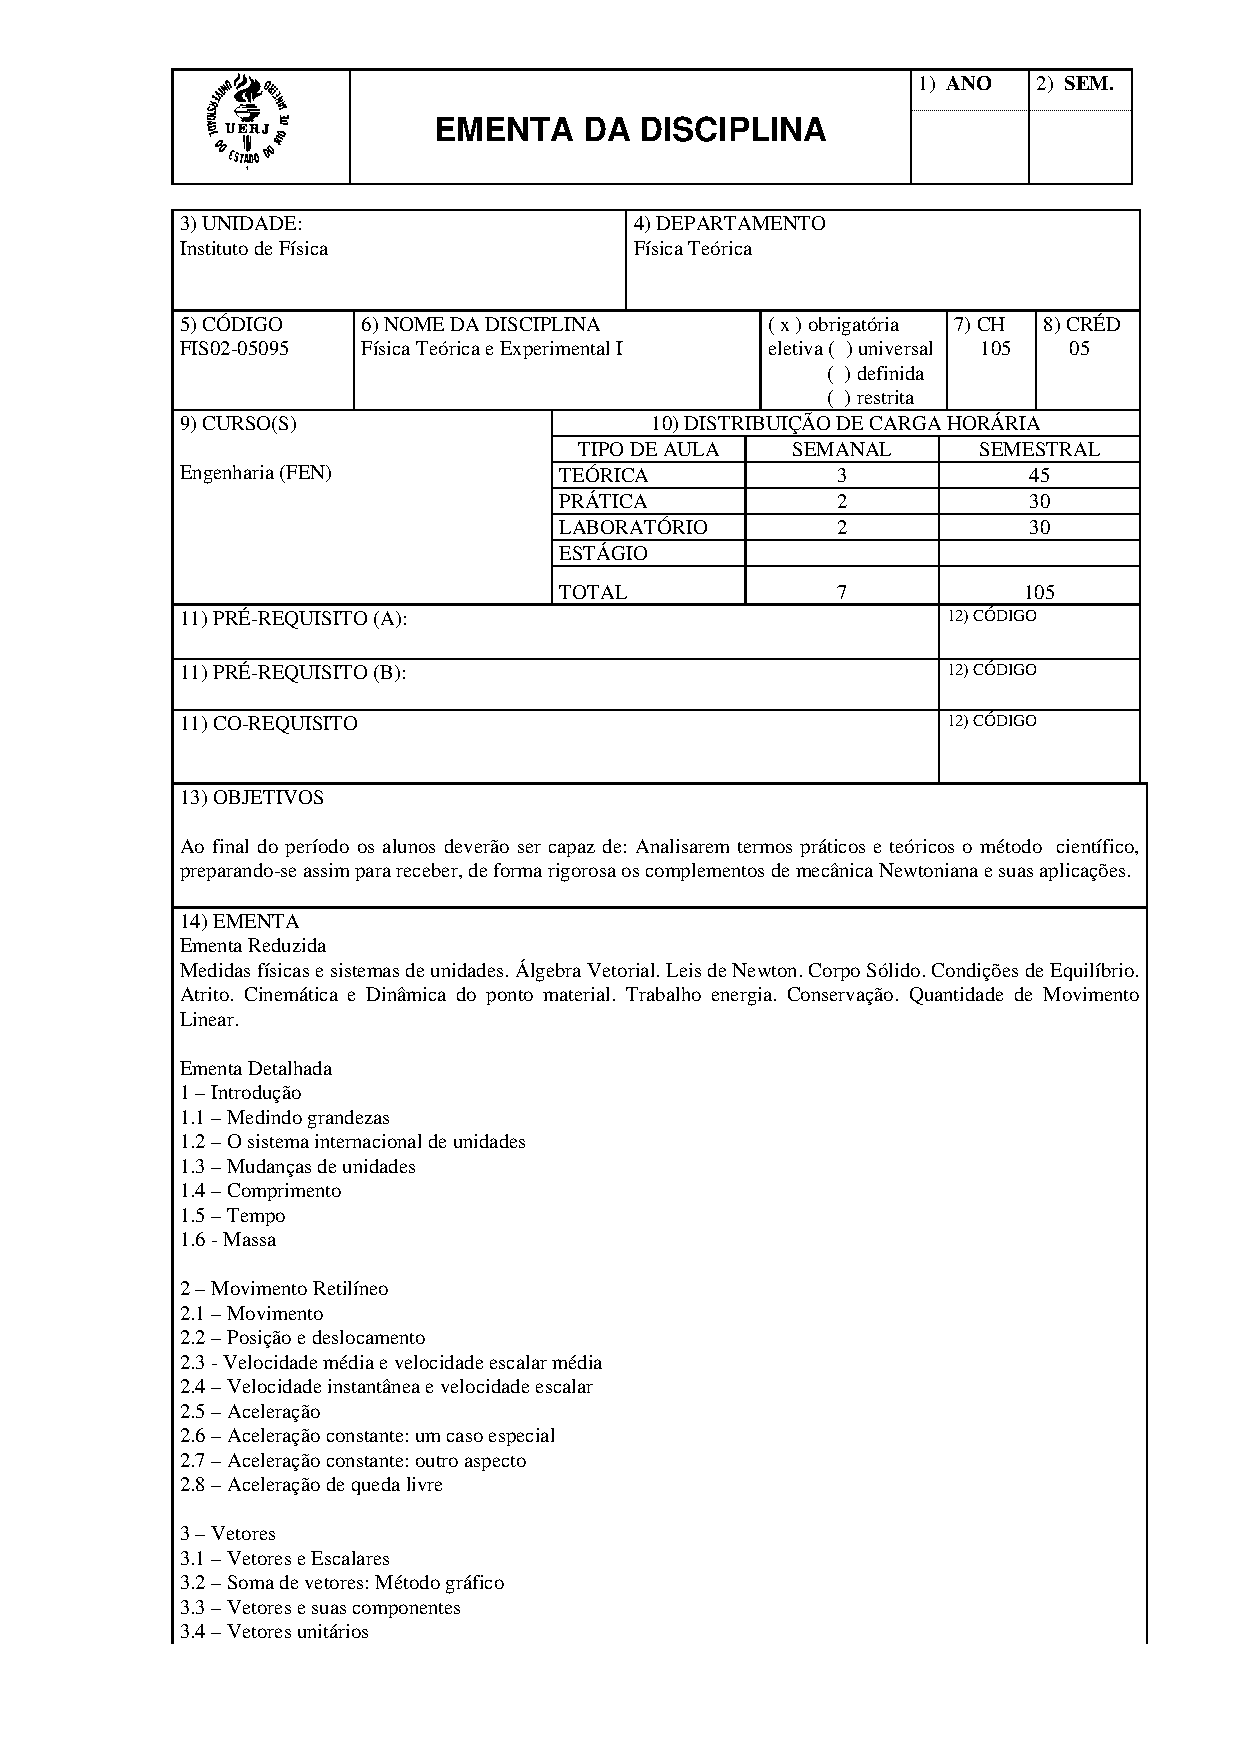
\includepdf[pages=-,addtotoc={1,section,1,{\FisI},},pagecommand={\thispagestyle{fancy}}]{ementasExternas/FisicaI.pdf}
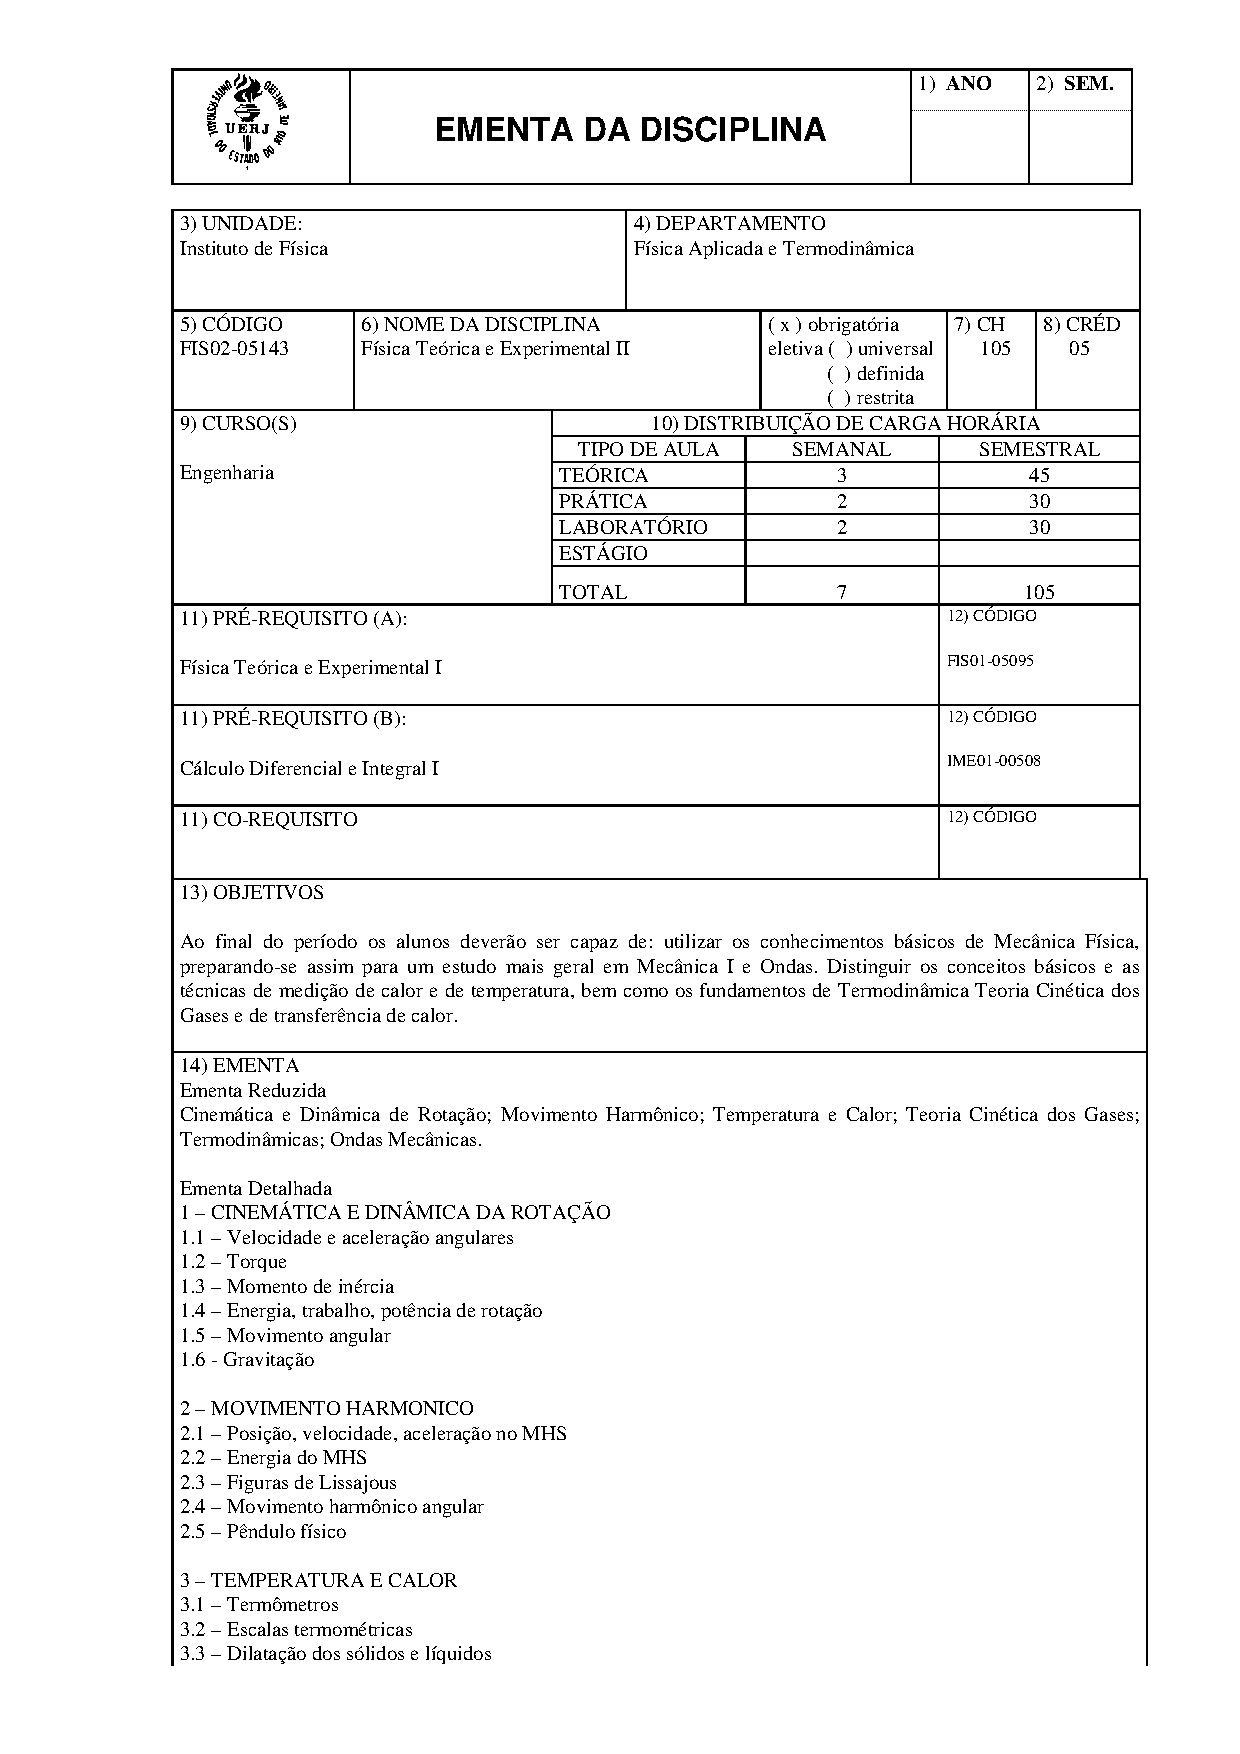
\includepdf[pages=-,addtotoc={1,section,1,{\FisII},},pagecommand={\thispagestyle{fancy}}]{ementasExternas/FisicaII.pdf}
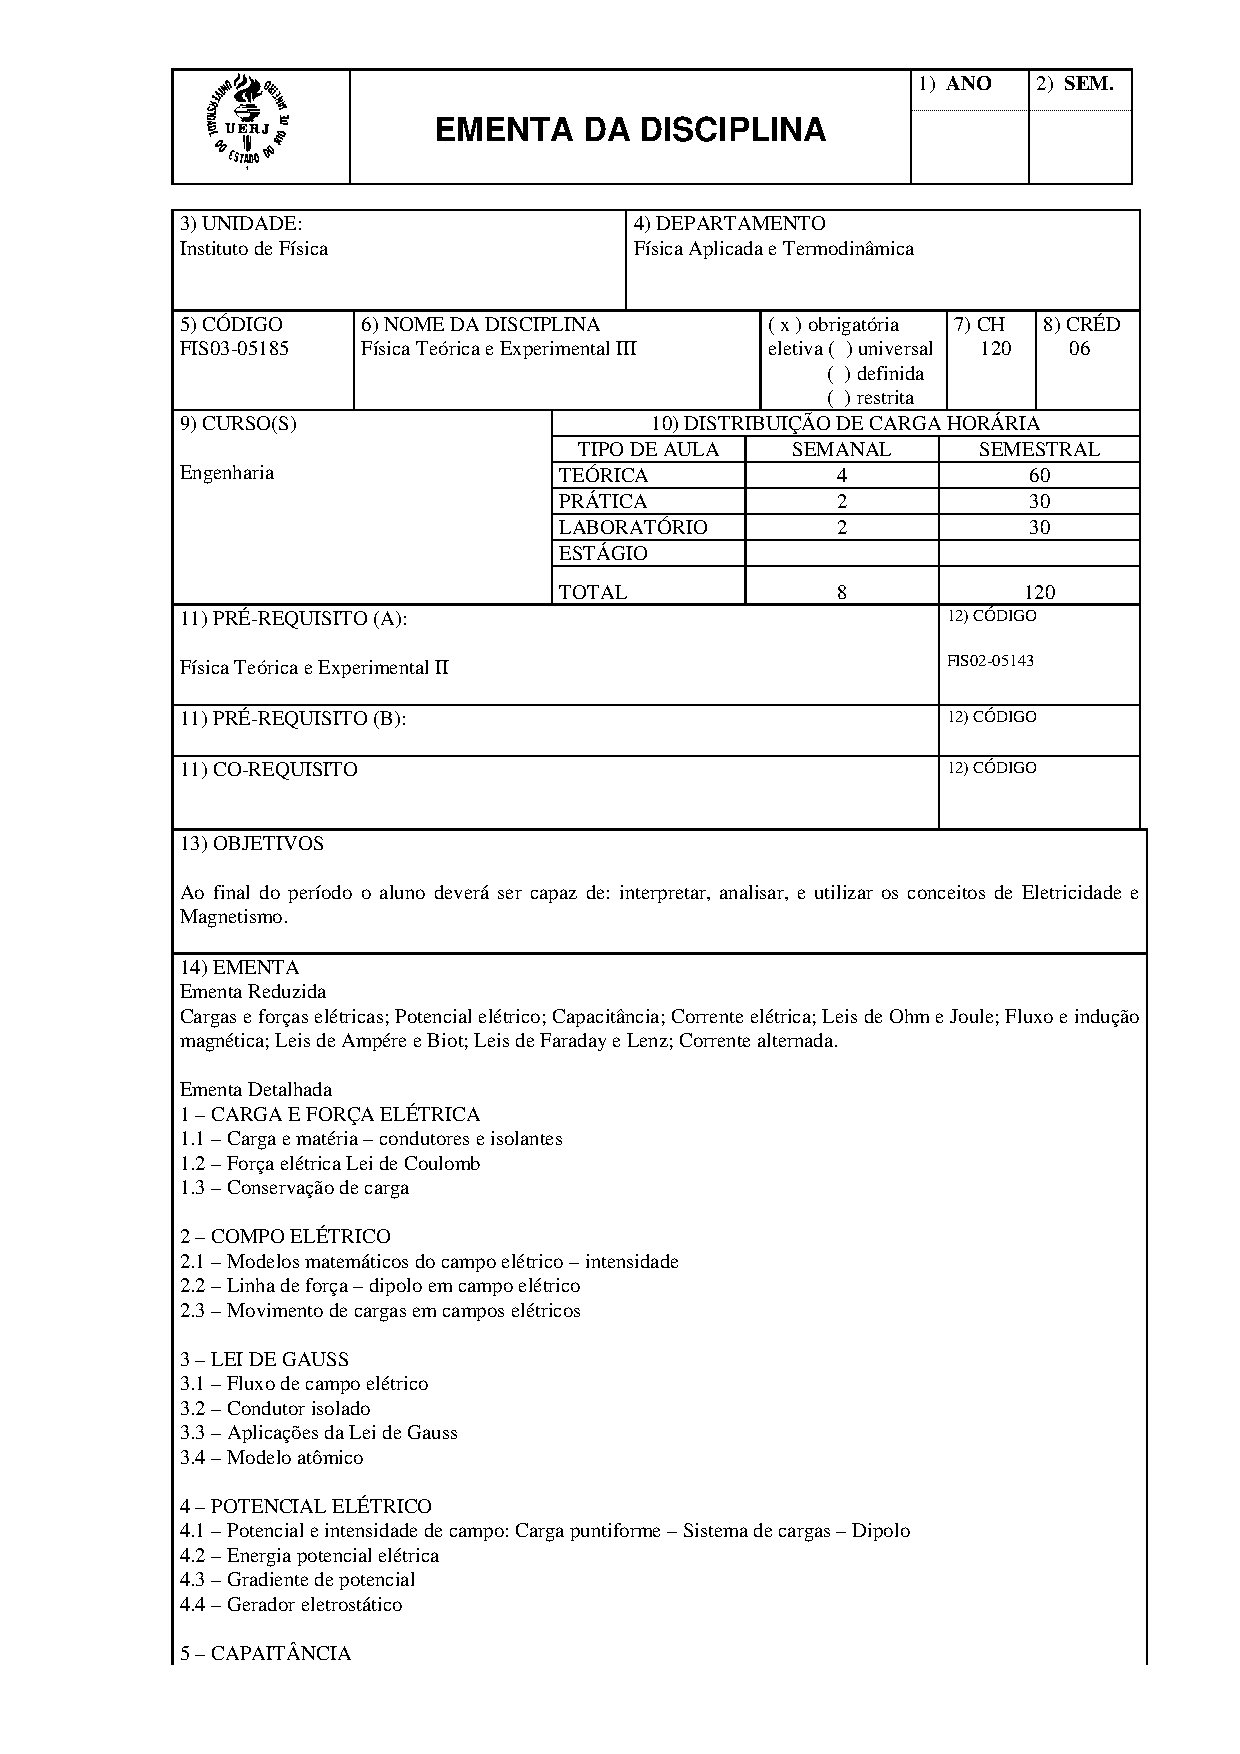
\includepdf[pages=-,addtotoc={1,section,1,{\FisIII},},pagecommand={\thispagestyle{fancy}}]{ementasExternas/FisicaIII.pdf}
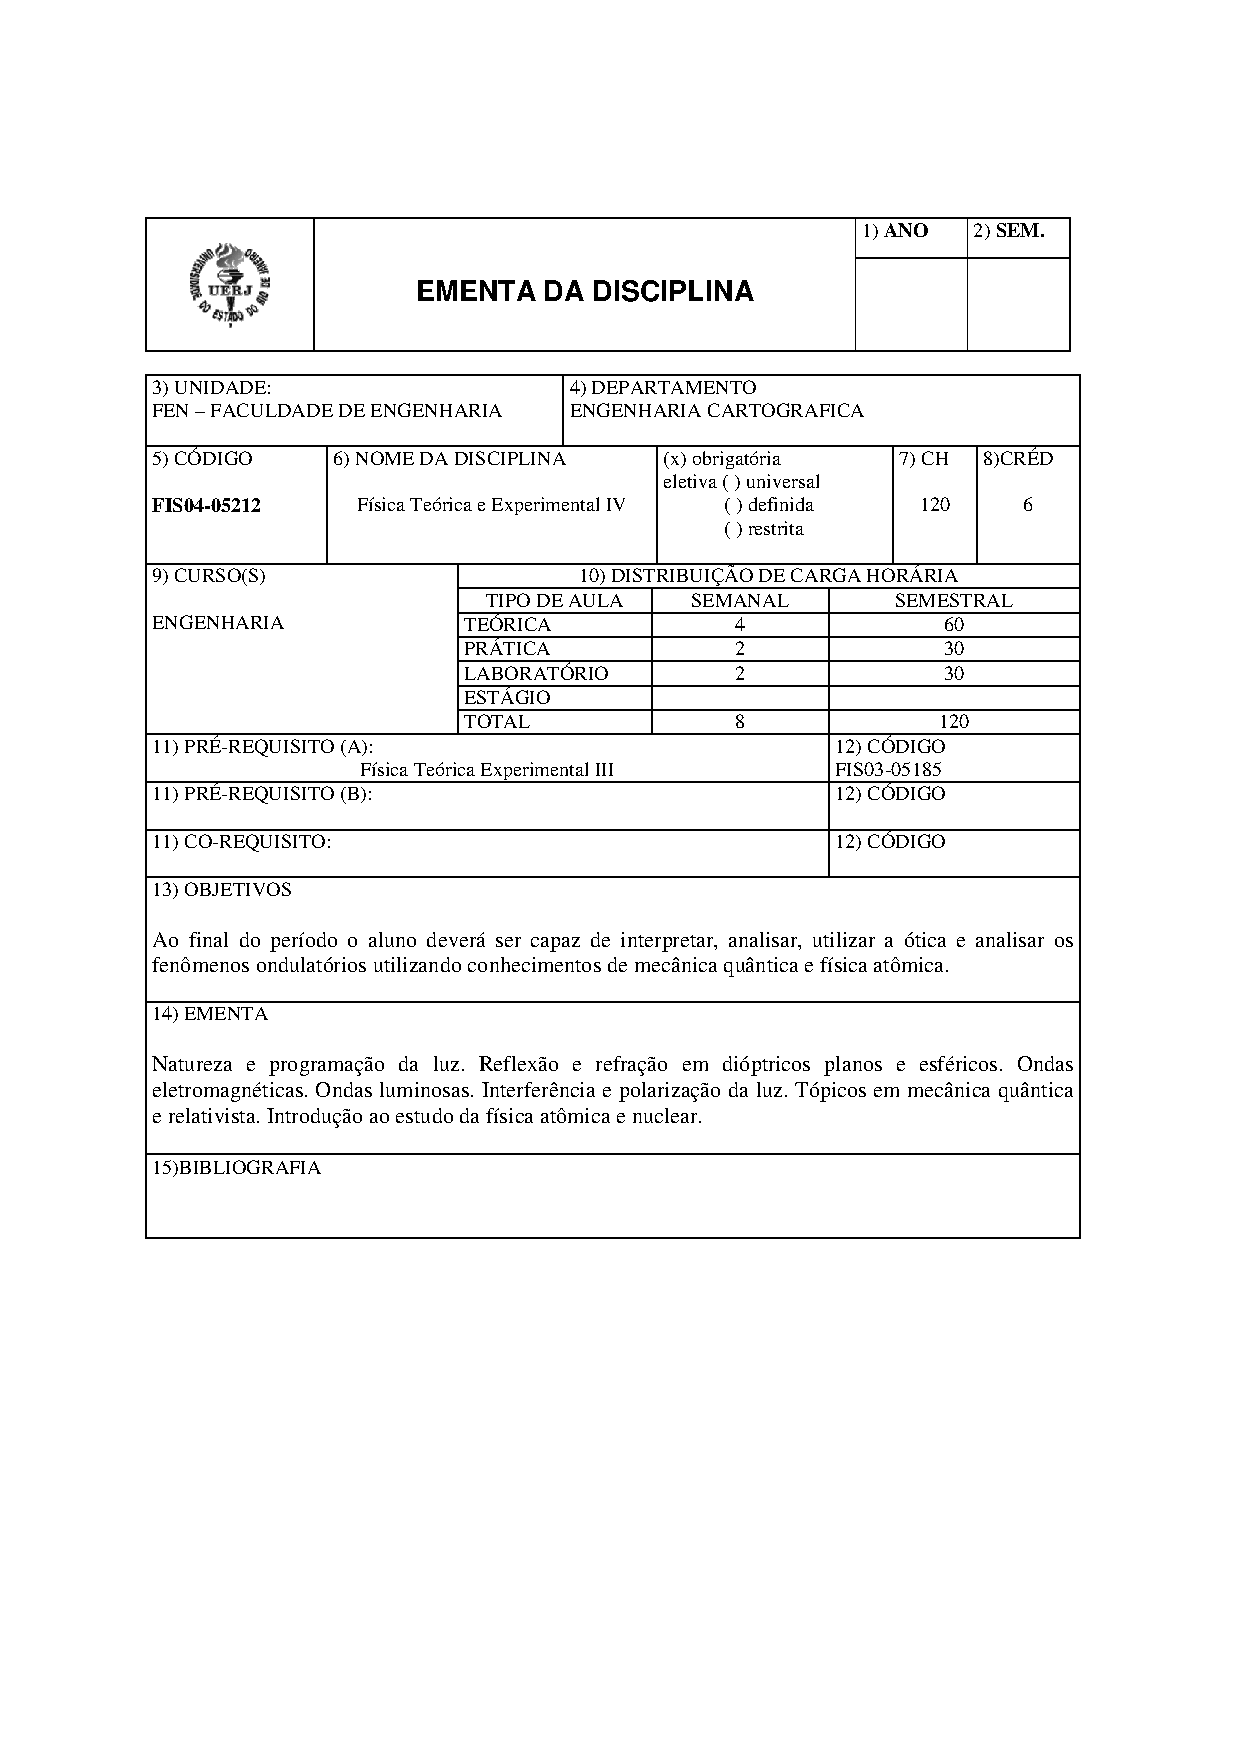
\includepdf[pages=-,addtotoc={1,section,1,{\FisIV},},pagecommand={\thispagestyle{fancy}}]{ementasExternas/FisicaIV.pdf}

\includepdf[pages=-,addtotoc={1,section,1,{\FundComp},},pagecommand={\thispagestyle{fancy}}]{pdf/FundamentosDeComputadores.pdf}
\includepdf[pages=-,addtotoc={1,section,1,{\EletGeo},},pagecommand={\thispagestyle{fancy}}]{pdf/Eletiva3_Geomatica.pdf}
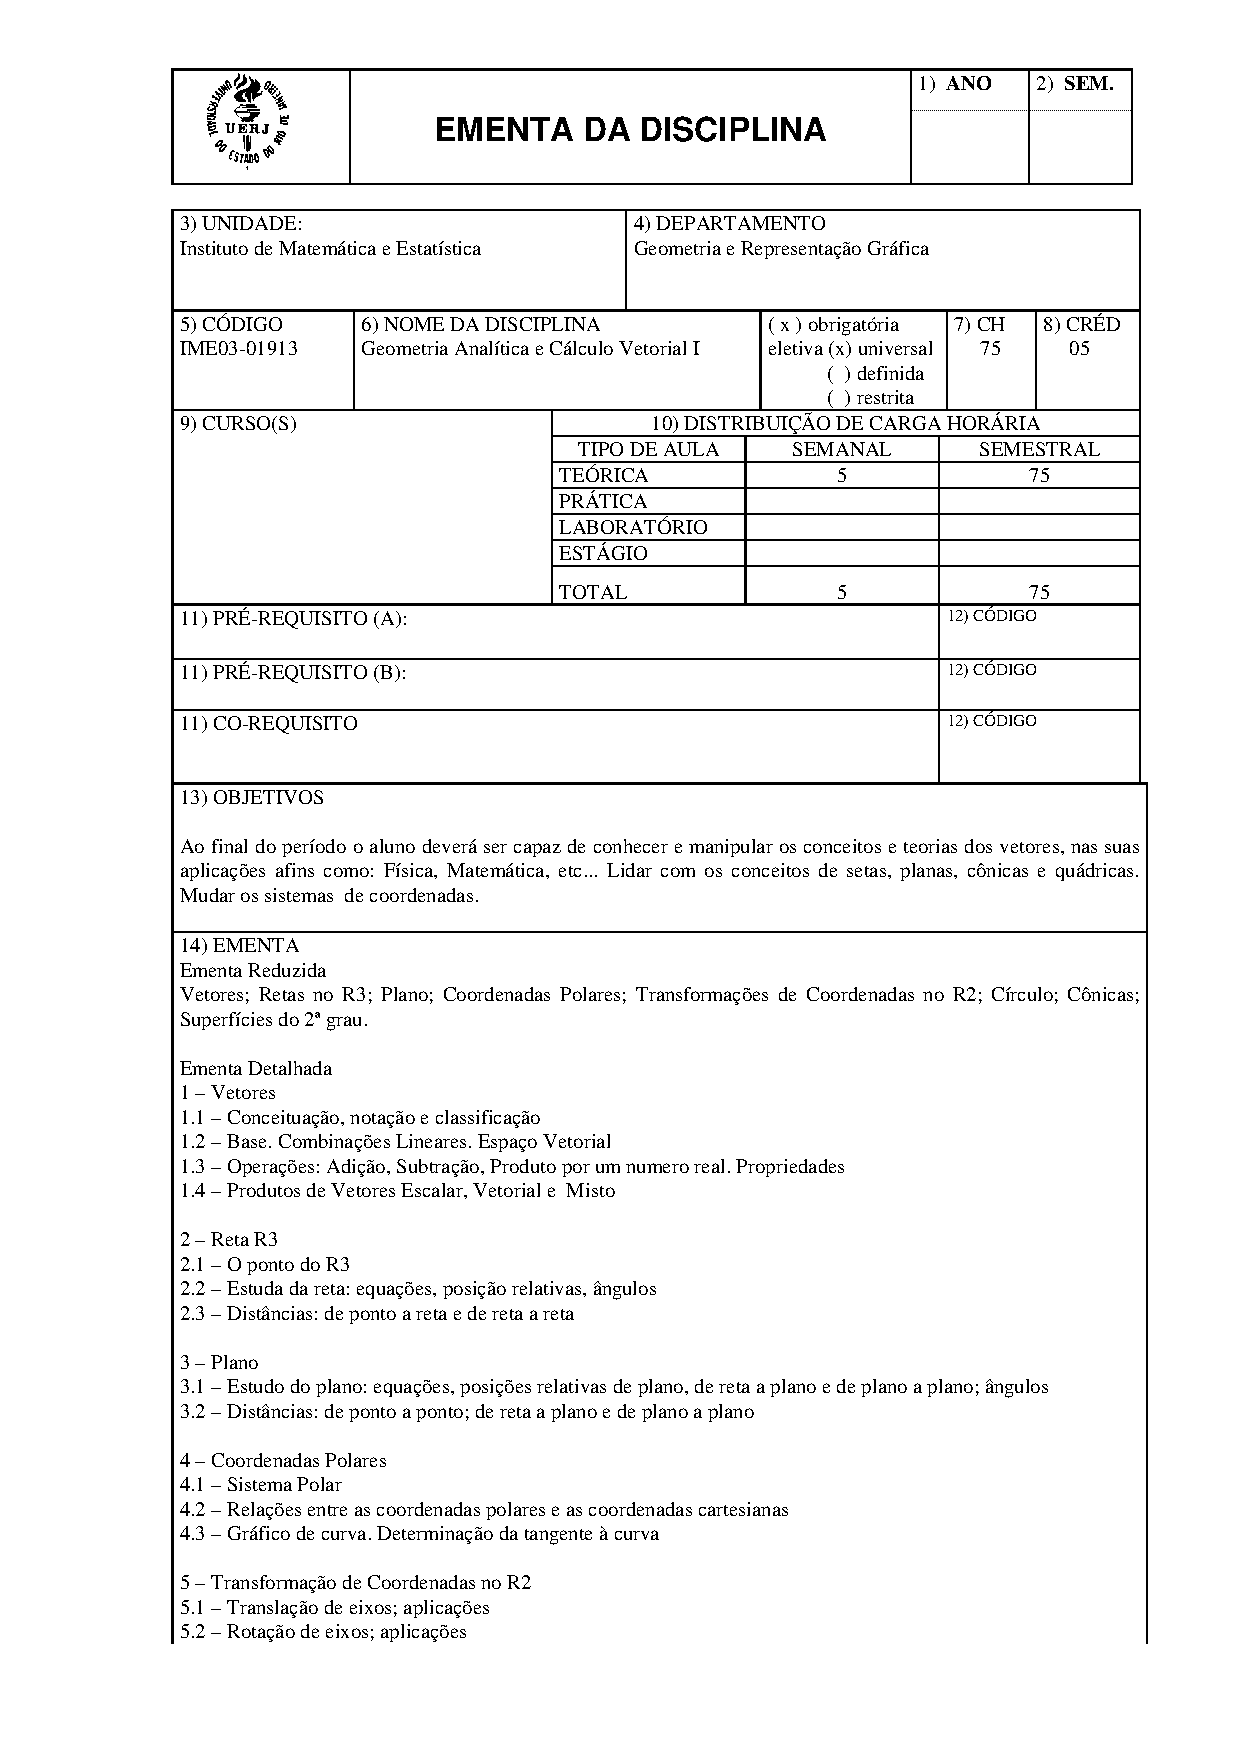
\includepdf[pages=-,addtotoc={1,section,1,{\GeoAna},},pagecommand={\thispagestyle{fancy}}]{ementasExternas/GeometriaAnalitica.pdf}
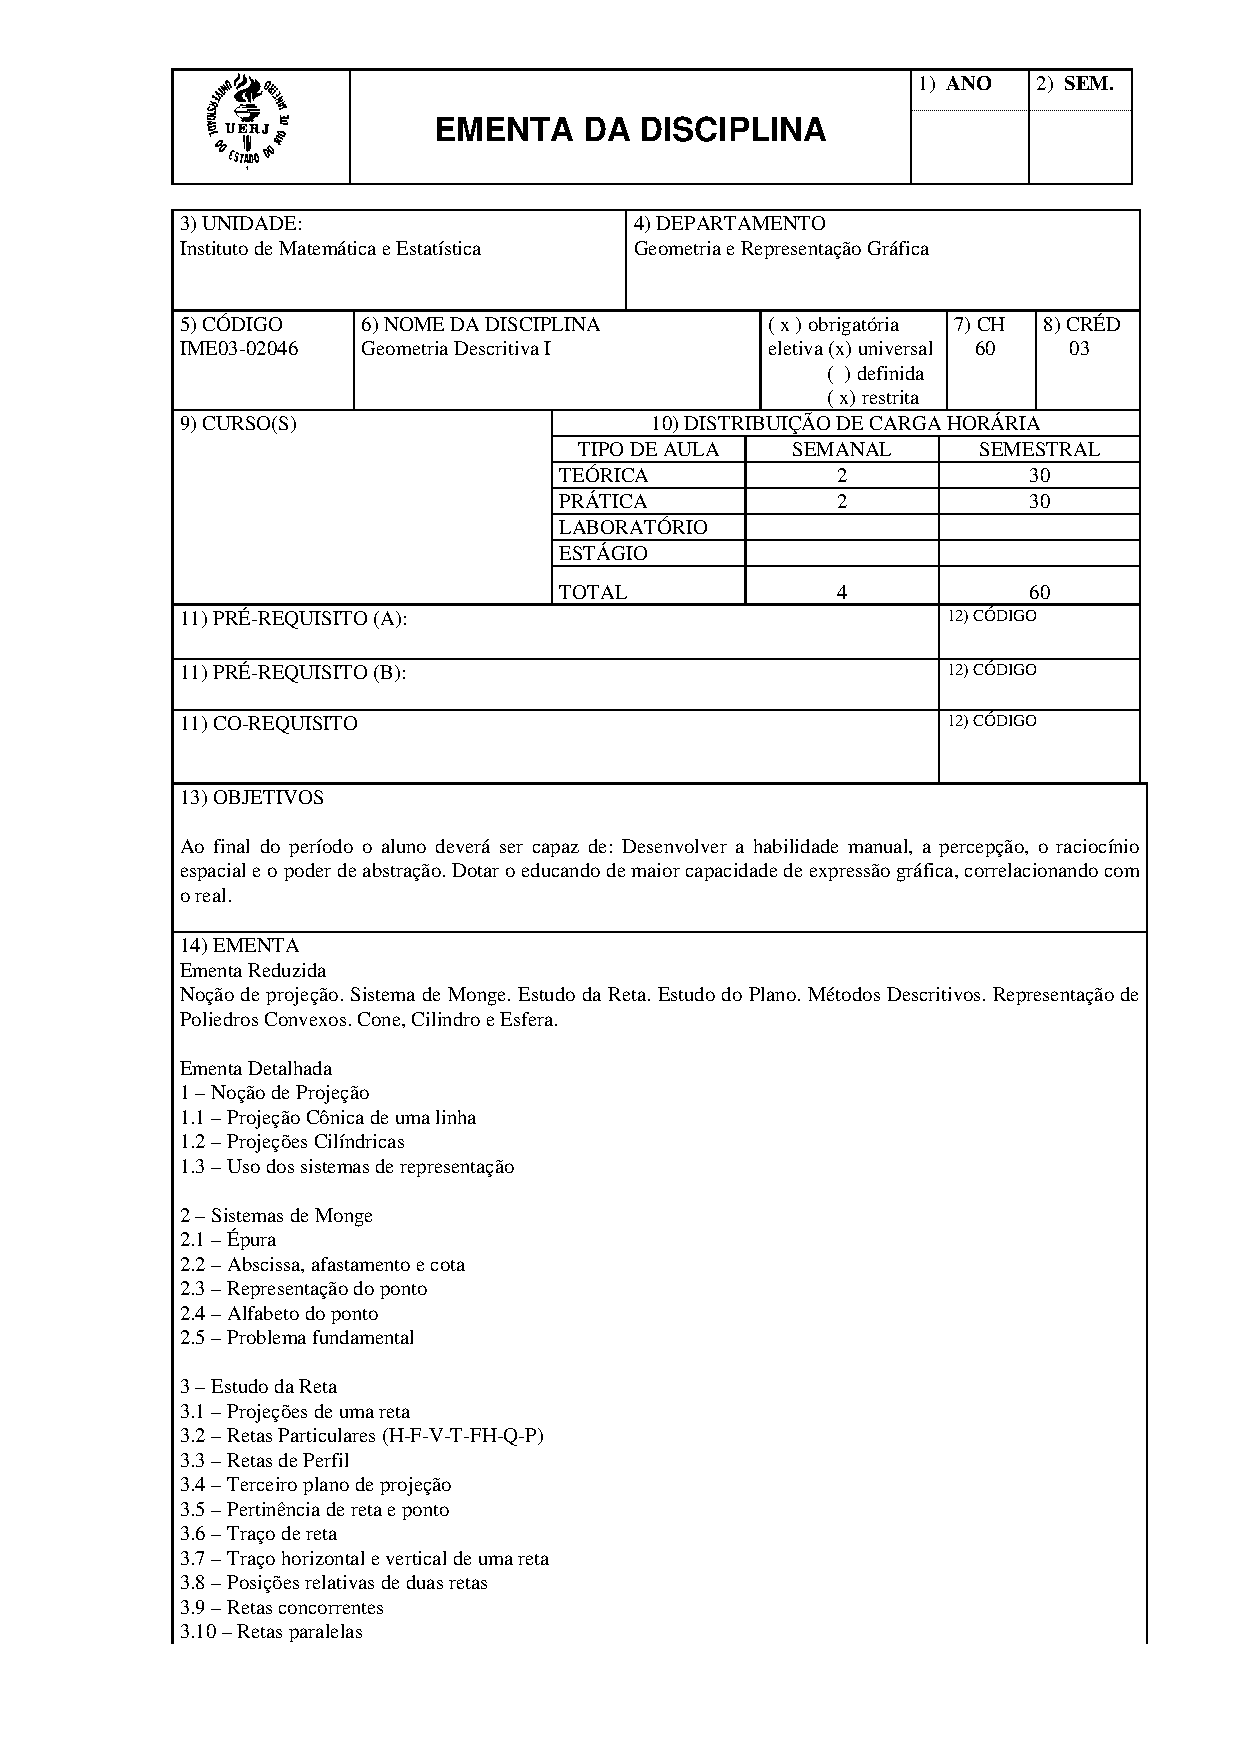
\includepdf[pages=-,addtotoc={1,section,1,{\GDSName},},pagecommand={\thispagestyle{fancy}}]{ementasExternas/GeometriaDescritivaI.pdf}
\includepdf[pages=-,addtotoc={1,section,1,{\IC},},pagecommand={\thispagestyle{fancy}}]{pdf/InteligenciaComputacional.pdf}

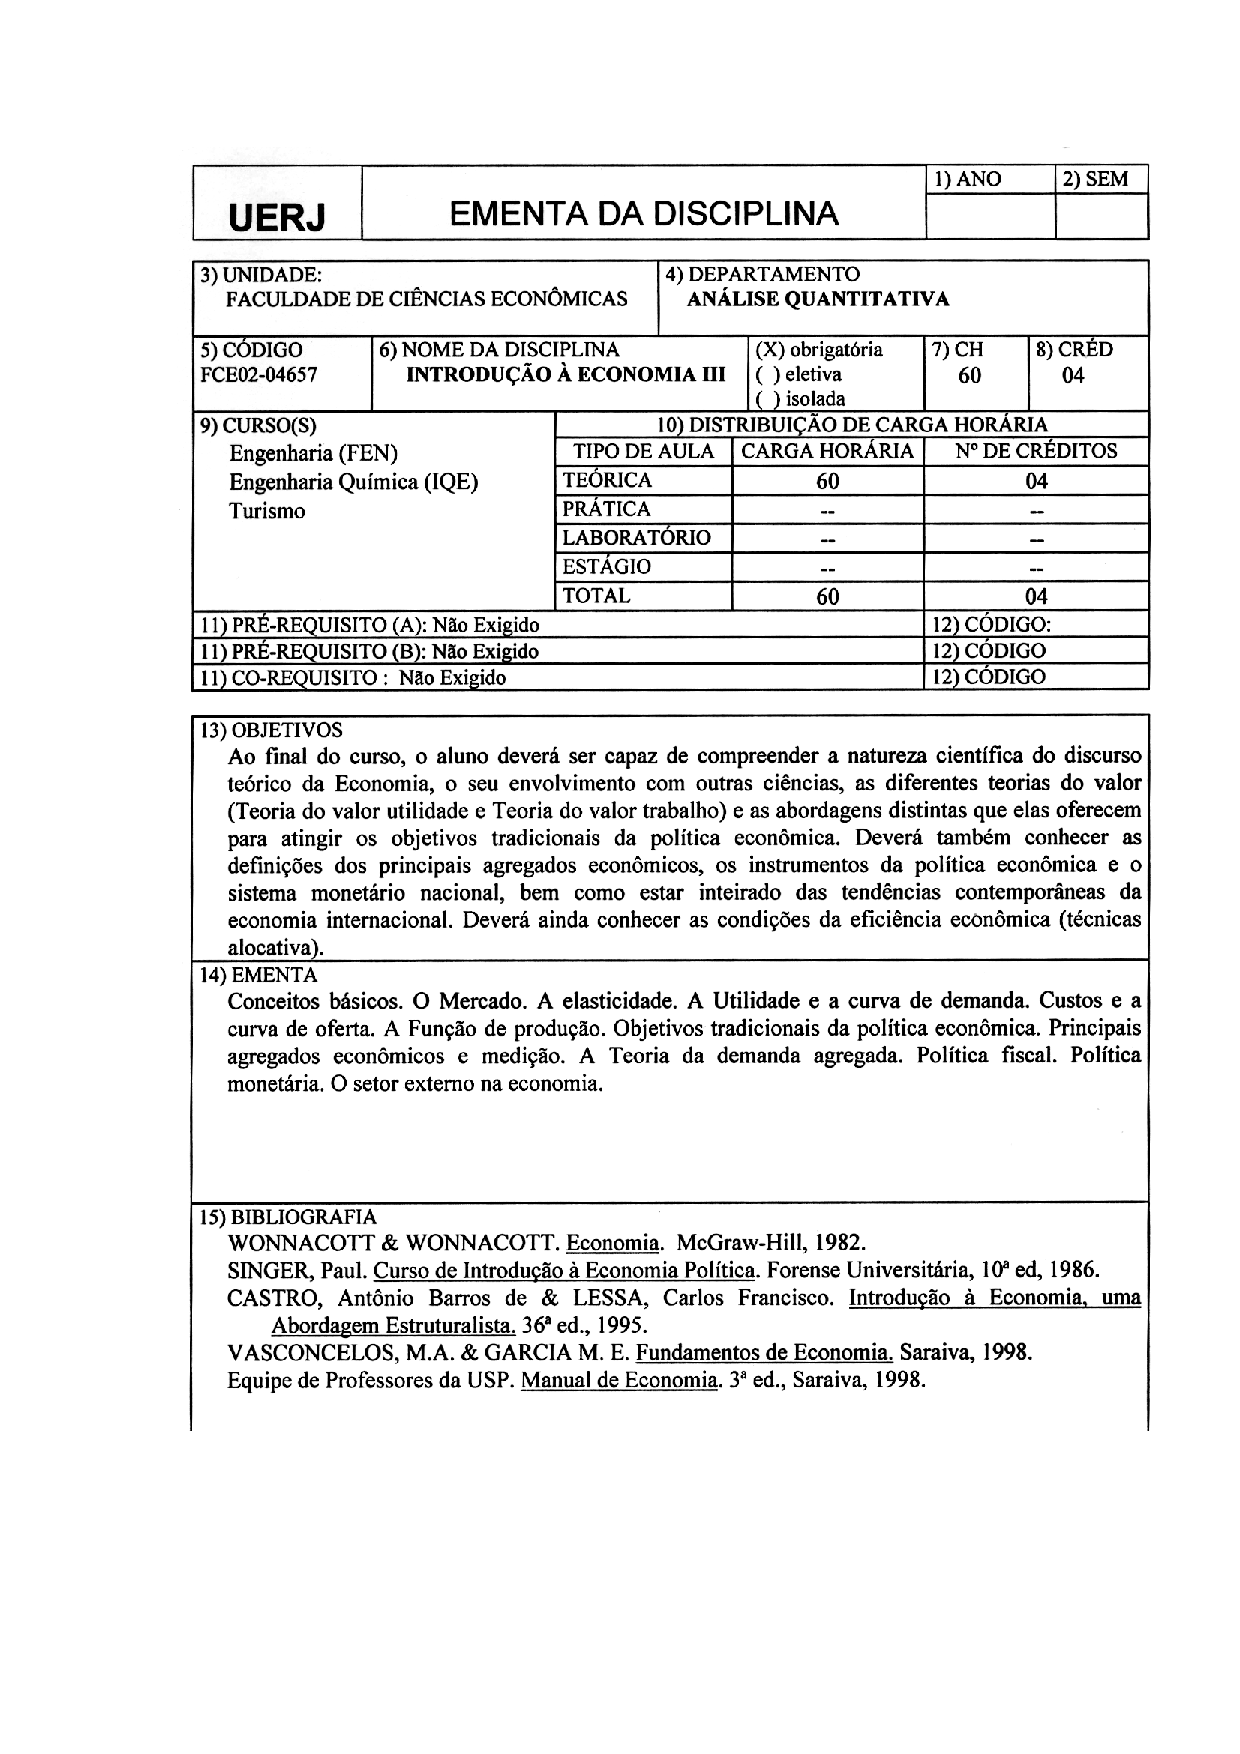
\includepdf[pages=-,addtotoc={1,section,1,{\IntEco},},pagecommand={\thispagestyle{fancy}}]{ementasExternas/IntroducaoAEconomia.pdf}
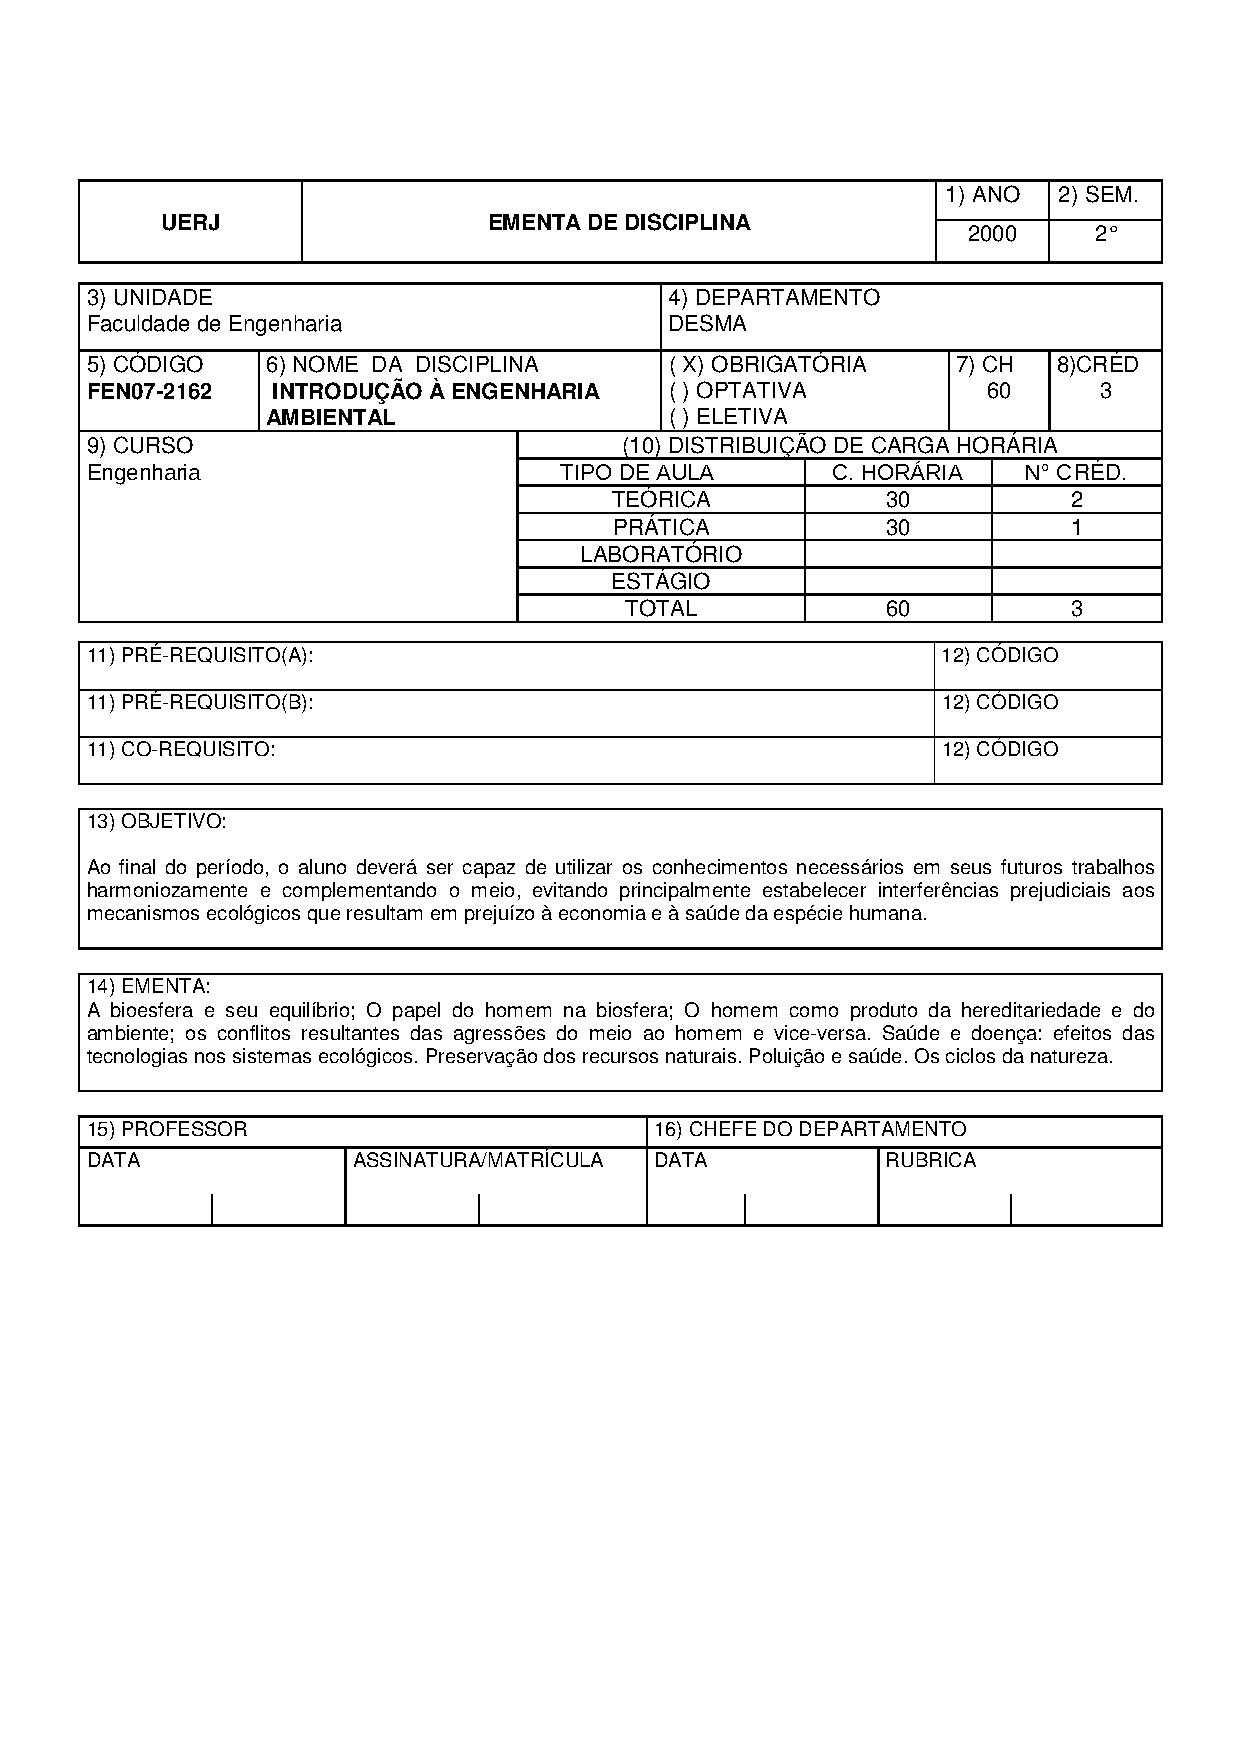
\includepdf[pages=-,addtotoc={1,section,1,{\IntAmb},},pagecommand={\thispagestyle{fancy}}]{ementasExternas/IntroducaoAEngenhariaAmbiental.pdf}
\includepdf[pages=-,addtotoc={1,section,1,{\LabProgA},},pagecommand={\thispagestyle{fancy}}]{pdf/LaboratorioDeProgramacaoA.pdf}
\includepdf[pages=-,addtotoc={1,section,1,{\LabProgB},},pagecommand={\thispagestyle{fancy}}]{pdf/LaboratorioDeProgramacaoB.pdf}
\includepdf[pages=-,addtotoc={1,section,1,{\LogProg},},pagecommand={\thispagestyle{fancy}}]{pdf/LogicaEmProgramacao.pdf}

\includepdf[pages=-,addtotoc={1,section,1,{\MatEle},},pagecommand={\thispagestyle{fancy}}]{pdf/MateriaisEletricosEMagneticos.pdf}
\includepdf[pages=-,addtotoc={1,section,1,{\MecTec},},pagecommand={\thispagestyle{fancy}}]{ementasExternas/MecanicaTecnica.pdf}
\includepdf[pages=-,addtotoc={1,section,1,{\MetQuant},},pagecommand={\thispagestyle{fancy}}]{pdf/MetodosQuantitativos.pdf}
\includepdf[pages=-,addtotoc={1,section,1,{\MineraDados},},pagecommand={\thispagestyle{fancy}}]{pdf/MineracaoDeDados.pdf}
\includepdf[pages=-,addtotoc={1,section,1,{\ModMat},},pagecommand={\thispagestyle{fancy}}]{ementasExternas/ModelosMatematicos.pdf}

\includepdf[pages=-,addtotoc={1,section,1,{\EletPadroes},},pagecommand={\thispagestyle{fancy}}]{pdf/Eletiva6_Padroes.pdf}
\includepdf[pages=-,addtotoc={1,section,1,{\PrincTelec},},pagecommand={\thispagestyle{fancy}}]{ementasExternas/PrincipiosDeTelecomunicacoesIII.pdf}
\includepdf[pages=-,addtotoc={1,section,1,{\ProbEst},},pagecommand={\thispagestyle{fancy}}]{ementasExternas/ProbEst.pdf}
\includepdf[pages=-,addtotoc={1,section,1,{\ProcImag},},pagecommand={\thispagestyle{fancy}}]{pdf/ProcessamentoDeImagens.pdf}
\includepdf[pages=-,addtotoc={1,section,1,{\EletMov},},pagecommand={\thispagestyle{fancy}}]{pdf/Eletiva5_ProgramacaoParaDispositivosMoveis.pdf}

\includepdf[pages=-,addtotoc={1,section,1,{\ProjSO},},pagecommand={\thispagestyle{fancy}}]{pdf/ProjetoDeSistemasOperacionais.pdf}
\includepdf[pages=-,addtotoc={1,section,1,{\ProjA},},pagecommand={\thispagestyle{fancy}}]{pdf/ProjetoXIA.pdf}
\includepdf[pages=-,addtotoc={1,section,1,{\ProjB},},pagecommand={\thispagestyle{fancy}}]{pdf/ProjetoDeGraduacaoB.pdf}
\includepdf[pages=-,addtotoc={1,section,1,{\ProjBD},},pagecommand={\thispagestyle{fancy}}]{pdf/ProjetoEAdministracaoDeBancoDeDados.pdf}
\includepdf[pages=-,addtotoc={1,section,1,{\QuiX},},pagecommand={\thispagestyle{fancy}}]{ementasExternas/QuimicaX.pdf}

\includepdf[pages=-,addtotoc={1,section,1,{\EletRec},},pagecommand={\thispagestyle{fancy}}]{pdf/Eletiva1_ReconhecimentoDePadroes.pdf}
\includepdf[pages=-,addtotoc={1,section,1,{\EletRedes},},pagecommand={\thispagestyle{fancy}}]{pdf/Eletiva2_RedesDeInterconexao.pdf}
\includepdf[pages=-,addtotoc={1,section,1,{\ResMat},},pagecommand={\thispagestyle{fancy}}]{ementasExternas/ResMat.pdf}
\includepdf[pages=-,addtotoc={1,section,1,{\SistEmb},},pagecommand={\thispagestyle{fancy}}]{pdf/SistemasEmbutidos.pdf}
\includepdf[pages=-,addtotoc={1,section,1,{\Telep},},pagecommand={\thispagestyle{fancy}}]{pdf/TeleprocessamentoERedes.pdf}

\includepdf[pages=-,addtotoc={1,section,1,{\TeoComp},},pagecommand={\thispagestyle{fancy}}]{pdf/TeoriaDeCompiladores.pdf}


\addappheadtotoc


%\printindex

%%%%%%%%%%%%%%%%%%%%%%%%%%%%%%%%%%%%%%%%%%%%%%%%%%%%%%%%%%%%%%%%%%%%%%

\end{document}





